\section{Teoria della calcolabilità}

\subsection{Funzioni primitivo ricorsive}
Vorremmo definire la classe delle funzioni implementabili in un calcolatore, tale classe è stata definita in vari modi,
ad inizio '900 da Church, Turing, Post e altri, e si è poi visto che le varie definizioni date erano equivalenti, seppur magari non fosse quella
l'intenzione originaria di chi le aveva date. Le principali definizioni che vediamo e che sono state date, sono:
\begin{enumerate}
    \item tramite gli operatori di chiusura,
    \item tramite un modello di calcolo (macchine di Turing),
    \item tramite formule aritmetiche.
\end{enumerate}

\begin{definition}[Funzioni primitive ricorsive - PRF]
    Definiamo la classe delle \vocab{funzioni primitive ricorsive} a partire da alcune funzioni di base e chiudendo la classe sotto alcune operazioni di chiusura.
    Le funzioni di base vanno da $\NN^k \to \NN$ per qualche $k \in \NN$ e sono:
    \begin{itemize}
        \item $0_k : \NN^k \to \NN$, per ogni $k \in \NN$, tale che $0_k(x_1, \dots, x_k) = 0_k(\mathbf x) = 0$,
        \item $s : \NN \to \NN$, la funzione successore, $s(x) = x + 1$,
        \item $\pi_{k,i} : \NN^k \to \NN$, per ogni $k \in \NN$ e $1 \leq i \leq k$, tale che $\pi_{k,i}(x_1, \dots, x_k) = x_i$.
    \end{itemize}
    Chiudiamo queste funzioni di base sotto le seguenti operazioni, siano $f : \NN^a \to \NN$ e $g_1, \dots, g_a : \NN^b \to \NN$ primitive ricorsive, allora:
    \[ \NN^b \to \NN : (x_1, \dots, x_b) \mapsto f(g_1(x_1, \dots, x_b), \dots, g_a(x_1, \dots, x_b)) \]
    è una funzione primitiva ricorsiva, cioè chiudiamo sotto composizione; siano $h : \NN^{k} \to \NN$ e $g : \NN^{k+2} \to \NN$ primitive ricorsive, allora:
    \[ f : \NN^{k+1} \to \NN : \begin{cases}
        f(0,y_1, \dots, y_k) = h(y_1, \dots, y_k) \\
        f(x+1,y_1, \dots, y_k) = g(x,f(x,y_1, \dots, y_k),y_1, \dots, y_k)
    \end{cases}
    \]
    è primitiva ricorsiva, cioè chiudiamo sotto ricorsione.
\end{definition}

\begin{remark}[Permutazione di primitive ricorsive]
    Sia $f(x_1, \dots, x_k)$ primitiva ricorsiva, e sia $\sigma \in \mathrm S_k$ una permutazione, allora:
    \[ g(x_1, \dots, x_k) := f(x_{\sigma(1)}, \dots, x_{\sigma(k)}) \]
    è primitiva ricorsiva, infatti $g$ si ottiene da $f$ componendo con le proiezioni relative alla permutazione $\sigma$:
    \[ g(x_1, \dots, x_k) = f(\pi_{k,\sigma(1)}(x_1, \dots, x_k), \dots, \pi_{k,\sigma(k)}(x_1, \dots, x_k)) \]
    Anzi non è necessario che $\sigma$ sia una permutazione, basta che sia una qualsiasi funzione da $\{1, \dots, k\}$ a $\{1, \dots, k\}$.
\end{remark}

\begin{notation}[PR]
    D'ora in avanti PR sarà l'abbreviazione di ``primitivo ricorsivo/a''.
\end{notation}

Vediamo alcuni esempi di funzioni primitive ricorsive.

\begin{example}[Funzioni costanti]
    Qualsiasi funzione costante $c_m : \NN^k \to \NN$ è primitiva ricorsiva, infatti $c_m$ si ottiene da $0_k$ componendo con la funzione successore $s$ un numero finito di volte:
    \[ c_m(x_1, \dots, x_k) = s^m \circ 0_k(x_1, \dots, x_k) \]
\end{example}

\begin{example}[Funzione somma]
    La funzione somma $f(x,y) = x + y$ è primitiva ricorsiva, infatti è definita per ricorsione sulla $x$ a partire da $h(y) := \pi_{1,1}(y)$ e $g(x,z,y) := s \circ \pi_{3,2}(x,z,y)$:
    \[ f(x,y) := \begin{cases}
        f(0,y) = h(y) = \pi_{1,1}(y) = y \\
        f(x+1,y) = g(x,f(x,y),y) = s \circ \pi_{3,2}(x,f(x,y),y) = s(f(x,y))
    \end{cases}\]
\end{example}

\begin{example}[Funzione prodotto]
    La funzione prodotto $f(x,y) = x \cdot y$ è primitiva ricorsiva, infatti è definita per ricorsione sulla $x$ a partire da $h(y) := 0_1(y)$ e $g(x,y,z) := \pi_{3,2}(x,y,z) + \pi_{3,3}(x,y,z)$ (che è PR perché è composizione di funzioni PR):
    \[ f(x,y) := \begin{cases}
        f(0,y) = h(y) = 0_1(y) = 0 \\
        f(x+1,y) = g(x,f(x,y),y) = f(x,y) + y
    \end{cases}\]
\end{example}

\begin{example}[Funzione potenza]
    La funzione potenza $f(x,y) = x^y$ è primitiva ricorsiva, infatti posso definire $f(x,y) := F(y,x)$, dove $F$ è definita per ricorsione usando $h(x) := s \circ 0_1(x) = c_1$ e $g(a,b,c) = \pi_{3,2}(a,b,c) \cdot \pi_{3,3}(a,b,c)$:
    \[ F(y,x) := \begin{cases}
        F(0,x) = h(x) = c_1(x) = 1 \\
        F(y+1,x) = g(y,F(y,x),x) = F(y,x) \cdot x
    \end{cases} \]
\end{example}

\enlargethispage{2\baselineskip}
\begin{example}[Funzione predecessore]
    Definiamo la funzione \vocab{predecessore} $\pred$ come:
    \[ \pred(x) := \begin{cases}
        0 & \text{se $x = 0$} \\
        x - 1 & \text{se $x > 0$}
    \end{cases} \]
    $\pred$ è primitiva ricorsiva, ed è definita per ricorsione da $h := 0_0$ e $g(x,z) := \pi_{2,1}(x,z)$:
    \[ \pred(x) := \begin{cases}
        \pred(0) = h(0) = 0_0(0) = 0 \\
        \pred(x+1) = g(x,\pred(x)) = \pi_{2,1}(x,\pred(x)) = x
    \end{cases} \]
\end{example}

\begin{example}[Sottrazione troncata]
    Definiamo la funzione \vocab{sottrazione troncata} $\dotminus$ come:
    \[ x \dotminus y := \begin{cases}
        0 & \text{se $x \leq y$} \\
        x - y & \text{se $x > y$}
    \end{cases} \]
    $\dotminus$ è primitiva ricorsiva, infatti è definita per ricorsione sulla $y$ a partire da
    $h(x) := \pi_{1,1}(x)$ e $g(a,b,c) := \pred \circ \pi_{3,2}(a,b,c)$:
    \[ x \dotminus y := \begin{cases}
        x \dotminus 0 = h(x) = \pi_{1,1}(x) = x \\
        x \dotminus (y+1) = g(y,x \dotminus y,x) = \pred \circ \pi_{3,2}(y,x \dotminus y,x) = \pred(x \dotminus y)
    \end{cases} \]
    Notare come stia facendo ricorsione sull'altra variabile, e non su $x$, ma, come già visto, a meno di permutare, posso fare ricorsione su qualsiasi variabile, quindi è ininfluente.
\end{example}

\begin{definition}[Predicato]
    $P \subseteq \NN^k$ è un \vocab{predicato PR} se esiste una funzione $f : \NN^k \to \NN$ PR tale che:
    \[ f(\mathbf x) = \begin{cases}
        0 & \text{se $\mathbf x \in P$} \\
        1 & \text{se $\mathbf x \notin P$}
     \end{cases} \]
\end{definition}

\begin{notation}[Notazione per i predicati]
    Eventualmente si confonderanno le notazioni $\mathbf x \in P$ e $P(\bf x)$, intendendo con $P(\bf x)$ la formula $f(\mathbf x) = 0$.
\end{notation}

\begin{example}[Il predicato $\texttt{zerop}$]
    Un esempio di predicato è $\texttt{zerop} := \{0\}$, infatti è definito dalla funzione PR:
    \[ f(x) := 1 \dotminus (1 \dotminus x) \] 
    infatti, se $\NN\ni x > 1$ allora $1 \dotminus x = 0$ e $1 \dotminus 0 = 1$, per cui $x \not\in \texttt{zerop}$; se $x = 1$ vale ancora $f(1)=1$, mentre se $x = 0$ si ha $1 \dotminus 0 = 1$ e $1 \dotminus 1 = 0$, quindi $x \in \texttt{zerop}$.
\end{example}

\begin{remark}[Algebra di boole dei predicati PR]
    I predicati PR sottoinsiemi dello stesso $\NN^k$ formano un'algebra di boole.
\end{remark}

\begin{proof}
    Dati $P, Q \subseteq \NN^k$ predicati PR devo verificare che i seguenti sono predicati PR: $P^\complement$, $P \cup Q$, $\NN^k$.
    \begin{itemize}
        \item[$\boxed{\NN^k}$] È un predicato prendendo la funzione PR data da $0_k$.
        \item[$\boxed{P^\complement}$] Sia $f$ la funzione PR che definisce $P$, allora $P^\complement$ è definito dalla funzione PR $1 \dotminus f$.
        \item[$\boxed{P \cup Q}$] Siano $f$ e $g$ le funzioni PR che definiscono rispettivamente $P$ e $Q$, allora $P \cup Q$ è definito dalla funzione PR $(1 \dotminus ((1 \dotminus f) + (1 \dotminus g)))$, oppure da $f \cdot g$.
    \end{itemize}
\end{proof}

\begin{example}[Insiemi di confronto]
    Gli insiemi $\{x \leq y\}$, $\{x < y\}$, $\{x = y\}$, $\{x \neq y\}$\footnote{Nel senso di $\{(x,y) \in \NN^2 |\ldots\}$.} sono predicati PR.
    Per $\{x = y\}$ è sufficiente usare:
    \[ f(x,y) := 1 \dotminus (1 \dotminus (y \dotminus x + x \dotminus y)) \]
    da cui si ha subito anche che $\{x \ne y\}$ è un predicato PR, infatti $\{x \ne y\} = \{x = y\}^\complement$. Per $\{x \leq y\}$ si usa:
    \[ g(x,y) := x \dotminus y \]
    Mettendo assieme queste due cose si ottiene:
    \[ \{x < y\} = \{x \leq y\} \cap \{x \neq y\} \]
    simmetricamente per $\geq$ e $>$. Osservare, infine, che se al posto di $x$ e $y$ ci fossero $f(\mathbf x)$ e $g(\mathbf y)$ allora tutto funzionerebbe allo stesso modo, per le proprietà delle funzioni PR;
    pertanto gli insiemi di confronto sono predicati PR anche quando ci sono delle funzioni PR a definirli.
\end{example}

\begin{remark}[Definizione per casi di funzioni PR]
    Se $P \subseteq \NN^k$ è un predicato PR, e $f, g : \NN^k \to \NN$ sono funzioni PR, allora la funzione definita per casi da:
    \[ h(\mathbf x) := \begin{cases}
        f(\mathbf x) & \text{se $\mathbf x \in P$} \\
        g(\mathbf x) & \text{se $\mathbf x \notin P$}
    \end{cases} \]
    è una funzione PR, infatti posso scrivere $h$ come: $h(\mathbf x) = f(\mathbf x) \cdot (1 \dotminus P(\mathbf x)) + g(\mathbf x) \cdot P(\mathbf x)$, che è una composizione di funzioni PR, e quindi è PR.\\
    Notare che possiamo anche usare più predicati PR per definizioni con più casi, usando sempre lo schema sopra ed annidando le definizioni.
\end{remark}

\begin{example}[Funzione modulo]
    La funzione $x \bmod y = z \overset{\text{def}}{\iff} z < y \land y \mid x - z$, cioè il rappresentante di $x$ modulo $y$, è una funzione PR poiché è definita per ricorsione e per casi:
    \[ x \bmod y := \begin{cases}
        0 \bmod y = 0 \\
        (x+1) \bmod y := \begin{cases}
            0 & \text{se $x \bmod y + 1 = y$} \\
            (x \bmod y) + 1 & \text{se $x \bmod y + 1 \ne y$}
        \end{cases}
    \end{cases} \]
    cioè, visto che $x = qy + x \mod y$, allora $x+1 = qy + (x \mod y + 1)$, per cui se $x \mod y + 1 = y$ allora $x+1 = (q+1)y + 0$, altrimenti $x+1 = qy + (x \mod y + 1)$.
    Osservare inoltre che nella definizione per casi abbiamo usato il predicato PR $P(b,c) := \{b + 1 = c\}$, e la $h$ per la ricorsione:
    \[ h(a,b,c) := \begin{cases}
        0 & \text{se $b + 1 = c$} \\
        b + 1 & \text{se $b + 1 \ne c$}
    \end{cases} \]
    che è una funzione PR per definizione per casi.
\end{example}
\pagebreak
\begingroup
\setlength{\abovedisplayskip}{5pt plus 1pt minus 2pt}
\setlength{\belowdisplayskip}{5pt plus 1pt minus 2pt}
\setlength{\abovedisplayshortskip}{3pt plus 1pt minus 1pt}
\setlength{\belowdisplayshortskip}{3pt plus 1pt minus 1pt}
\setlength{\jot}{2pt}
\begin{remark}[Somma dei valori di una funzione PR sotto un certo punto]
    Sia $f : \NN^{k+1} \to \NN$ una funzione PR, allora la funzione:
    \[ (y_1, \dots, y_k,x) \mapsto \sum_{i < x} f(y_1, \dots, y_k, i) \]
    è PR, infatti è definita per ricorsione a partire dalle funzioni PR $h(y_1, \dots, y_k) := 0$ e $g(a,b,d_1, \dots, d_k) := b + f(d_1, \dots, d_k, a)$:
    \[ \sum_{i < x} f(y_1, \dots, y_k, i) := \begin{cases}
        \sum_{i < 0} f(y_1, \dots, y_k, i) &= h(y_1, \dots, y_k) = 0 \\
        \sum_{i < x+1} f(y_1, \dots, y_k, i) &= \sum_{i < x} f(y_1, \dots, y_k, i) \\ &+ f(y_1, \dots, y_k,x) 
    \end{cases} \]
\end{remark}

\begin{example}[Funzione che conta gli elementi del predicato fino ad $x$]
    Sia $P \subseteq \NN^{k+1}$ un predicato PR, allora la funzione:
    \[ g : (y_1, \dots, y_k,x) \mapsto \#\{(y_1, \dots, y_k, i) \in P : i < x\}\] 
    è una funzione PR, infatti:
    \[ g(y_1, \dots, y_k,x) = \sum_{i < x} (1 \dotminus P(y_1, \dots, y_k, i))
    \]
\end{example}

\begin{example}[Appartenenza ad un altro predicato sotto un certo punto]
    Definiamo il predicato $Q \subseteq \NN^{k+1}$ come:
    \[ (y_1, \dots, y_k,x) \in Q \iff \exists i < x \; (y_1, \dots, y_k,i) \in P\]
    con $P \subseteq \NN^{k+1}$ predicato PR. Tale sottoinsieme è un predicato PR in quanto è possibile definirlo come insieme di confronto:
    \[ Q(y_1, \dots, y_k,x) = \{g(y_1, \dots, y_k,x) > 0\} \]
    dove $g(y_1, \dots, y_k,x) = \#\{(y_1, \dots, y_k, i) \in P : i < x\}$ è la funzione PR che conta gli elementi del predicato $P$ sotto $x$.
\end{example}

\begin{example}[Funzione quoziente intero]
    Definiamo $x \div y := \floor{\displaystyle\frac{x}{y}}$, con la convenzione $x \div 0 := 0$.
    La funzione $x \div y$ è PR, può essere definita per ricorsione primitiva:
    \[ \begin{cases}
        0 \div y := 0 \\
        (x+1) \div y := \begin{cases}
            0 & \text{se $y = 0$} \\
            (x \div y) + 1 & \text{se $y \neq 0$ e $x \bmod y + 1 = y$} \\
            x \div y & \text{se $y \neq 0$ e $x \bmod y + 1 \ne y$}
        \end{cases}
    \end{cases} \]
    il predicato e la funzione usati per la ricorsione sono simili a quelli usati per definire il modulo, anche in questo caso vale che se $x = (x \div y)y + r$,
    allora $x+1 = (x \div y)y + (r+1)$, per cui se $r+1 = y$ allora $x+1 = (x \div y + 1)y + 0$, altrimenti $x+1 = (x \div y)y + (r+1)$.
\end{example}
\endgroup

\subsection{Codifica delle liste}

\begin{definition}[Pairing function]
    Definiamo la funzione \vocab{pairing function} - o funzione di accoppiamento, come:
    \[ \cons : \NN^2 \to \NN : (x,y) \mapsto \frac{(x+y)(x+y+1)}{2} + x + 1\]
\end{definition}

Tale funzione è biunivoca tra le coppie $(x,y) \in \NN^2$ e i numeri naturali maggiori o uguali a 1 - fa comodo avere un null point, e quindi non vogliamo che $(0,0)$ venga codificato da $0$.
La funzione di pairing si può pensare nel modo seguente:
\begin{figure}[htbp]
    \centering
    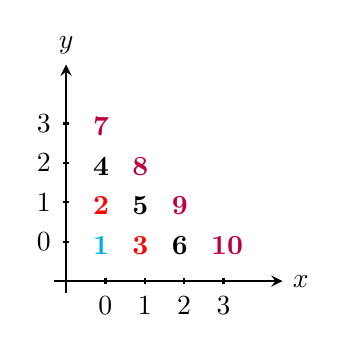
\begin{tikzpicture}[x=0.5cm, y=0.5cm, >=stealth]
        
        % Disegno degli assi x e y
        \draw[->, thick] (-0.3, 0) -- (5.5, 0) node[right] {$x$};
        \draw[->, thick] (0, -0.3) -- (0, 5.5) node[above] {$y$};
        
        % Tacche ed etichette sugli assi: a coordinate 1 corrisponde etichetta 0
        \foreach \i in {1,2,3,4} {
            \draw[thick] (\i,0.08) -- (\i,-0.08);
            \node[below=2pt] at (\i,0) {\number\numexpr\i-1\relax};
        }
        \foreach \j in {1,2,3,4} {
            \draw[thick] (0.08,\j) -- (-0.08,\j);
            \node[left=2pt] at (0,\j) {\number\numexpr\j-1\relax};
        }
        
        % Stile per i numeri: piu piccoli e ravvicinati ai punti interi
        \tikzset{numero/.style={font=\normalsize\bfseries, anchor=south west, xshift=-8pt, yshift=-8pt}}
        
        % Diagonale 1 - Ciano
        \node[numero, text=cyan] at (1, 1) {1};
        
        % Diagonale 2 - Rosso
        \node[numero, text=red] at (1, 2) {2};
        \node[numero, text=red] at (2, 1) {3};
        
        % Diagonale 3 - Nero
        \node[numero, text=black] at (1, 3) {4};
        \node[numero, text=black] at (2, 2) {5};
        \node[numero, text=black] at (3, 1) {6};
        
        % Diagonale 4 - Viola
        \node[numero, text=purple] at (1, 4) {7};
        \node[numero, text=purple] at (2, 3) {8};
        \node[numero, text=purple] at (3, 2) {9};
        \node[numero, text=purple] at (4, 1) {10};
        
        % --- Linee guida opzionali ---
        % Rimuovi i commenti dalle righe seguenti se desideri aggiungere 
        % delle leggere linee tratteggiate per enfatizzare le diagonali.
        % \draw[help lines, color=black!15, dashed] (0.6, 1.4) -- (1.4, 0.6);
        % \draw[help lines, color=black!15, dashed] (0.6, 2.4) -- (2.4, 0.6);
        % \draw[help lines, color=black!15, dashed] (0.6, 3.4) -- (3.4, 0.6);
        % \draw[help lines, color=black!15, dashed] (0.6, 4.4) -- (4.4, 0.6);
        
    \end{tikzpicture}
\end{figure}

\begin{definition}[Funzioni inverse di $\cons$]
    Definiamo le funzioni $\car, \cdr : \NN \to \NN$ come le funzioni inverse di $\cons$, ovvero:
    \begin{align*}
        \car(\cons(x,y)) & := x \\
        \cdr(\cons(x,y)) & := y
    \end{align*}
    tali funzioni sono PR, un modo per verificarlo è osservare che possono essere scritte come:
    \begin{align*}
        \car(z) = \sum_{i < z} \sum_{j < z} i \cdot (1 \dotminus \{z = \cons(i,j)\}) \\
        \cdr(z) = \sum_{i < z} \sum_{j < z} j \cdot (1 \dotminus \{z = \cons(i,j)\})
    \end{align*}
    cioè itero la somma finché non becco la coppia $(i,j)$ tale che $z = \cons(i,j)$, allora i due predicati danno 0 e quindi viene $1 \cdot i$ o $1 \cdot j$.
\end{definition}

\begin{exercise}[Funzione di Ackermann]
    Dimostrare che la funzione di Ackermann non è una funzione primitiva ricorsiva:\footnote{\underline{\textbf{Hint}}: Un qualunque programma costituito solo da cicli \texttt{for} annidati un numero finito di volte, e senza ricorsione, non può catturare l'intera funzione.}
    \[ A(m,n) := \begin{cases}
        A(0,n) = n + 1 \\
        A(m+1,0) = A(m,1) \\
        A(m+1,n+1) = A(m, A(m+1,n))
    \end{cases} \]
\end{exercise}

\begin{figure}[H]
    \centering
    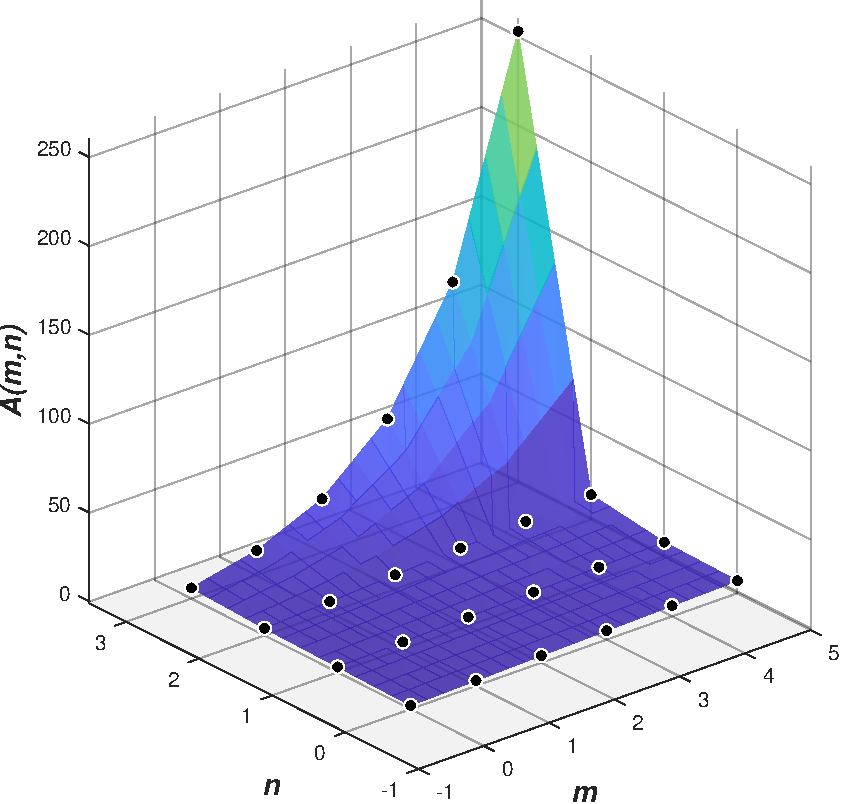
\includegraphics[width=0.45\textwidth]{Immagini/Ackermann.pdf}
    \caption{Plot della funzione di Ackermann}
\end{figure}

\begin{remark}[Le sezioni $n \mapsto A(m,n)$ sono PR]
    Per ogni $m \in \NN$, la funzione $A_m : \NN \to \NN$ definita da $A_m(n) := A(m,n)$ è PR.
    Si dimostra per induzione su $m$: $A_0(n)=n+1$ è il successore, e se $A_m$ è PR allora anche $A_{m+1}$ è PR, perché è definita per ricorsione da:
    \[ A_{m+1}(0) = A_m(1), \qquad A_{m+1}(n+1) = A_m(A_{m+1}(n)) \]
\end{remark}

L'idea che abbiamo voluto catturare, mediante le funzioni primitive ricorsive, è quella di una classe di funzioni che può essere implementata
in un calcolatore solo per mezzo di cicli \texttt{for} - per cui sarà già a priori fissato il numero di loop, e che non usino né i costrutti della ricorsione (quindi una funzione non può chiamare se stessa) e 
né usi cicli potenzialmente illimitati, come i cicli \texttt{while}.

\subsection{Funzioni ricorsive}

Definiamo inizialmente della notazione per rappresentare funzioni che non convergono.

\begin{definition}[$\NN_\bot$]
    Definiamo $\NN_\bot := \NN \cup \{\bot\}$.
\end{definition}

\begin{definition}[Funzioni ricorsive]
    Definiamo le \vocab{funzioni ricorsive} come le funzioni $f : \NN_\bot^k \to \NN_\bot$ a partire da alcune funzioni di base e chiudendo la classe sotto alcune operazioni di chiusura.
    Le funzioni di base, fissato $k \in \NN$, vanno da $\NN_\bot^k \to \NN_\bot$ e sono:
    \begin{align*}
        \pi_{k,i}(x_1, \dots, x_k) &= \begin{cases}
            x_i & \text{se } x_1, \dots, x_k \in \NN \\
            \textcolor{purple}{\bot} & \text{altrimenti}
        \end{cases} \\
        s(x) &= \begin{cases}
            x + 1 & \text{se $x \in \NN$} \\
            \textcolor{purple}{\bot} & \text{se $x = \textcolor{purple}{\bot}$}
        \end{cases} \\
        0_k(x_1, \dots, x_k) &= \begin{cases}
            0 & \text{se } x_1, \dots, x_k \in \NN \\
            \textcolor{purple}{\bot} & \text{altrimenti}
        \end{cases}
    \end{align*}
    Partendo da queste funzioni faccio la chiusura per le operazioni di:
    \begin{itemize}
        \item composizione;
        \item ricorsione primitiva, con lo stesso schema visto per le funzioni PR, ma con l'aggiunta del caso $f(\textcolor{purple}{\bot},\ldots) := \textcolor{purple}{\bot}$;
        \item \vocab{minimizzazione}, ovvero se $f : \NN^{k+1} \to \NN_\bot$ è ricorsiva, allora la funzione:
        \begin{multline*}
            \purple{\mu_kf}(x_1, \dots, x_k) = a \in \NN \overset{\text{def}}{\iff} \\
             f(x_1, \dots, x_k, a) = 0 \land \forall i < a \; f(x_1, \dots, x_k, i) \in \NN\setminus\{0\}
        \end{multline*}
        in particolare $f(x_1, \dots, x_k, i)$ non è $\bot$; se non esistesse un tale $a$ allora poniamo $\mu_kf(x_1, \dots, x_k) := \textcolor{purple}{\bot}$. \textcolor{MidnightBlue}{Cioè $\mu_kf$ produce il valore $a$ tale che $f(x_1, \dots, x_k, a) = 0$, e tale $a$ è il minimo possibile 
        - l'idea che si vuole catturare è quella della convergenza di un algoritmo, che si ferma al passo $a$, quando $f$ produce 0, e se non si ferma allora $\mu_kf$ non converge e quindi la poniamo $\bot$.}
    \end{itemize}
\end{definition}

\begin{definition}[Funzioni ricorsive totali]
    Diciamo che $f : \NN_\bot^k \to \NN_\bot$ funzione ricorsiva è una \vocab{totale} se $\forall (x_1, \dots, x_k) \in \NN^k \; f(x_1, \dots, x_k) \in \NN$, cioè $f$ non produce mai $\bot$.
\end{definition}

\begin{remark}[Input $\bot$]
    Se $f$ è ricorsiva ed uno degli input è $\bot$, allora $f$ produce $\bot$:
    \[ f(x_1, \dots, x_{i-1}, \textcolor{purple}{\bot}, x_{i+1}, \dots, x_k) = \textcolor{purple}{\bot} \]
    per ogni $i \in \{1, \dots, k\}$.
\end{remark}

\begin{proof}
    Si procede per induzione sulla costruzione di $f$. I casi delle 3 funzioni di base sono banali per la definizione stessa.
    \begin{itemize}
        \item Per la composizione, se $f = h \circ (g_1, \dots, g_m)$, e uno degli input di $f$ è $\bot$, allora anche almeno uno dei $g_i$ dà $\bot$ per ipotesi induttiva, per cui $h$ produce $\bot$, ancora per ipotesi induttiva, e quindi $f$ è $\bot$.
        \item Per la ricorsione primitiva, se $f$ è definita per ricorsione da $h$ e $g$, e uno degli input di $f$ è $\bot$, allora anche uno degli input di $h$ o di $g$ è $\bot$, per cui $h$ o $g$ producono $\bot$ per ipotesi induttiva, e quindi anche $f$ dà $\bot$.
        \item Per la minimizzazione, se $f = \mu_kf'$, e uno degli input di $f$ è $\bot$, allora anche uno degli input di $f'$ è $\bot$, per cui $f'$ produce $\bot$ a prescindere dalla variabile per cui si minimizza, e non fornendo mai un valore in $\NN\setminus\{0\}$, il minimo 
        non esiste, e quindi anche $f$ è $\bot$ per definizione.
    \end{itemize}
\end{proof}

\begin{fact}[Inclusione tra le classi di funzioni ricorsive]
    Valgono le seguenti inclusioni, tutte strette:
    \[ \{\text{funzioni PR}\} \subsetneq \{\text{funzioni ricorsive totali}\} \subsetneq \{\text{funzioni ricorsive}\} \]
\end{fact}

\begin{proof}
    I contenimenti sono tutti banali per le definizioni date, vediamo solo i controesempi per mostrare che sono stretti.
    Per il secondo contenimento si osserva che $\mu_x s \equiv \textcolor{purple}{\bot}$, perché l'equazione $s(x)=0$ non ha soluzioni.
    Per il primo è sufficiente considerare la funzione di Ackermann - che termina sempre per come è definita.
\end{proof}
\pagebreak
\subsection{Macchine di Turing}

Vogliamo caratterizzare le funzioni ricorsive come esattamente quelle che sono implementabili da una Macchina di Turing.

\begin{definition}[Macchina di Turing - TM]
    Siano $\Sigma$ un insieme finito di \vocab{simboli}, $Q$ un insieme finito di \vocab{stati}, una \vocab{macchina di Turing} (\vocab{TM}) è 
    il dato di $\Sigma$, $Q$, di una \vocab{funzione di transizione}:
    \[ \delta : Q \times \Sigma \to Q \times \Sigma \times \{\textcolor{purple}{\leftarrow}, \textcolor{purple}{\downarrow}, \textcolor{purple}{\rightarrow}\} \]
    dove l'ultimo insieme si rappresenta formalmente con $\{0,1,2\}$ (con la corrispondenza in questo esatto ordine), ma è più comodo rappresentarlo con le frecce. Una \vocab{configurazione} è il dato di $(s,p,n)$ dove 
    $s \in Q$ è lo stato della TM, $p \in \NN$ la posizione, e $n \in \Sigma^*$\footnote{Questa è la notazione di Kleene.} la stringa (o meglio tutto il nastro) in cui ci troviamo, i.e. $n \in \Sigma^{\NN}$ che è quasi sempre 0, i.e. $\exists N \in \NN \; \forall i > N \; n(i) = 0$.\\
    Dico che la macchina di Turing $M$ passa da una configurazione all'altra:
    \[ (s,p,n) \overset{M}{\to} (s',p',n') \]
    se: $s' = \pi_{3,1} \circ \delta(s,n(p))$, $p' = (p + \pi_{3,3} \circ \delta(s,n(p))) \dotminus 1$ cioè la posizione finale è quella iniziale più 1 se la freccia è $\rightarrow$, è quella iniziale se la freccia è $\downarrow$, e $p-1$ se la freccia è $\leftarrow$ - dove la terza componente di $\delta$ è identificata col numero non con la freccia, e:
    \[ n'(i) = \begin{cases}
        n(i) & \text{se $i \ne p$} \\
        \pi_{3,2} \circ \delta(s,n(p)) & \text{se $i = p$}
    \end{cases} \]
    cioè scorrendo il nastro modifico solo la cella in cui mi trovo inizialmente, $n(p)$, lascio le altre uguali e mi sposto.
\end{definition}

\begin{definition}[Chiusura transitiva]
    Dico che $c = (s,p,n) \overset{M^*}{\to} c' = (s',p',n')$ è la \vocab{chiusura transitiva} di $c \overset{M}{\to} c'$, se esiste una sequenza finita di configurazioni $c_0, \dots, c_k$ tale che:
    \[ c_0 \overset{M}{\to} c_1 \overset{M}{\to} \dots \overset{M}{\to} c_k \]
    con $c_0 = c$ e $c_k = c'$.
\end{definition}

\begin{exercise}[TM che riconosce i palindromi]
    Costruire una TM, ovvero la tabella di transizione, che riceva in input:
    \[ 0110101010111\ldots1011\textcolor{purple}{2}000\ldots \]
    ed ha due stati terminali, $0$ e $0'$, e termina in $0$ se e solo se la stringa è palindroma. Operiamo nell'alfabeto $\Sigma = \{0,1,2\}$.
\end{exercise}

\begin{exercise}[Difficile]
    Dimostra che una TM come nell'esercizio precedente, termina, nel caso peggiore
    in $O(\text{lunghezza stringa}^2)$ mosse - con $O$ si intende $\leq kl^2 + o(l^2)$ per qualche $k > 0$.\footnote{\underline{\textbf{Hint}}: L'algoritmo più
    sensato da implementare è: sostituire il primo simbolo con 2, poi spostarsi fino alla fine della stringa, sostituire l'ultimo simbolo con 2, e poi tornare indietro fino al primo simbolo,
    ripetere finché non si sostituisce tutta la stringa con dei 2, oppure finché non si trova un simbolo diverso da quello sostituito con 2, per cui se la stringa è lunga $l$, allora si fanno $l$ passi per sostituire ciascun simbolo,
    e quindi $l^2$ passi in totale. Bisogna dimostrare che non si può fare meglio di così, l'idea è che se la stringa è palindroma, la taglio alla metà esatta e posso ricostruire la metà sinistra usando come 
    informazione tutta la successione di stati che ho ottenuto attraversando il confine. La TM deve attraversare il confine almeno $l/2$ volte, quindi decido di aggiungere un blocco di 0 tra la stringa e la metà riflessa,
    in modo che la TM non possa usare come informazione il numero di passi fatti, e quindi deve attraversare il confine almeno $l/2$ volte, e ogni volta deve fare almeno $l/2$ passi, per cui ottengo $O(l^2)$.}
\end{exercise}

\subsection{Funzioni Turing-computabili}

\begin{definition}[Turing-computabilità]
    Sia $f : \NN^k \to \NN_\bot$ una funzione, diciamo che è \vocab{Turing-computabile} se esiste una TM $M$, con:
    \begin{itemize}
        \item $\Sigma \supseteq \{0,1,\blacktriangleright\}$,
        \item $Q \supseteq \{0,1\}$, con 0 \vocab{stop} e 1 \vocab{start},
        \item $\delta(0,x) = (0,x,\downarrow)$, ovvero lo stato terminale rimane fermo, non cambia simbolo né si muove,
    \end{itemize}
    e tale per cui:
    \begin{itemize}
        \item se $f(x_1, \dots, x_k) = y$, allora $\textcolor{purple}{\inp(x_1, \dots, x_k)} \overset{M^*}{\to} \textcolor{purple}{\outp(y)}$, con $\inp(x_1, \dots, x_k)$ e $\outp(y)$ due configurazioni,
        \item se $f(x_1, \dots, x_k) = \textcolor{purple}{\bot}$, allora $\textcolor{purple}{\inp(x_1, \dots, x_k)} \not\overset{M^*}{\to} (0,\ldots)$, ovvero non termina in uno stato 0, dove avverrebbe lo stop, i.e. se non c'è un output non termina mai.
    \end{itemize}
    Dove:
    \[ \inp(x_1, \dots, x_k) := (1,0,\blacktriangleright\underbrace{111111}_{x_1}0\underbrace{1111}_{x_2}0\ldots0\underbrace{111}_{x_k}00\ldots) \in Q \times \NN \times \Sigma^* \]
    dove il numero $x_i$ è rappresentato da una sequenza di $x_i$ simboli 1 (notazione unaria) - tanti quanti il valore di $x_i$, e tra un numero e l'altro c'è uno 0; analogamente:
    \[ \outp(y) := (0,0,\blacktriangleright\underbrace{111\ldots1}_{y}00\ldots) \in Q \times \NN \times \Sigma^* \]
    dove $y$ è rappresentato da una sequenza di $y$ simboli 1, seguita da una sequenza infinita di 0.
\end{definition}

\begin{theorem}[Ricorsiva $\Rightarrow$ Turing-computabile]
    Se $f : \NN^k \to \NN_\bot$ è ricorsiva parziale, allora $f$ è Turing-computabile.
\end{theorem}

\textcolor{MidnightBlue}{L'idea sarà far vedere che le funzioni di base sono Turing-computabili, e che le funzioni Turing computabili sono chiuse per operazioni di composizione, ricorsione primitiva e minimizzazione.}
Iniziamo con un caso particolare.

\begin{example}[Composizione di funzioni Turing computabili]
        Siano $f,g : \NN \to \NN_\bot$ funzioni Turing computabili, verifichiamo che $h(x) := f(g(x))$ è Turing computabile.
\end{example}

Ciò che vorrei è, detta $G$ la macchina associata a $g$ e $F$ quella associata a $f$, è far partire $G$ dalla sequenza iniziale $\blacktriangleright$, farla terminare sempre a $\blacktriangleright$, e poi da qui far partire $F$ e farla arrivare a $\blacktriangleright$ nello stato $0_F$,
facendo queste cose avrei di fatto costruito una macchina $H$ che implementa $h$.
\begin{figure}[H]
    \centering
    \begin{minipage}[b]{0.35\textwidth}
        \centering
        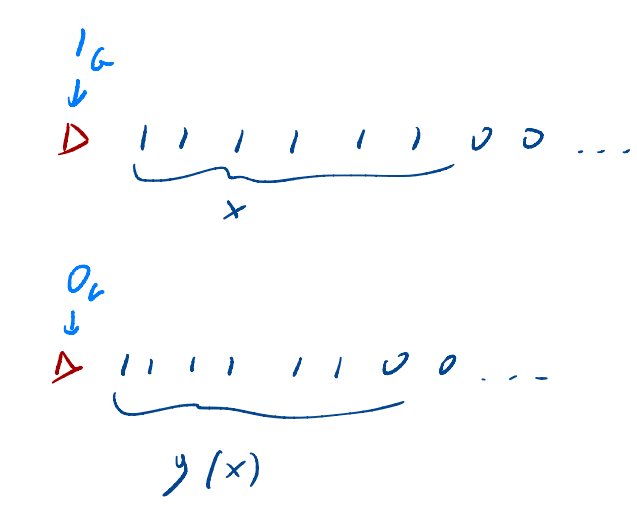
\includegraphics[width=\textwidth]{Immagini/composizione_di_TC_1.png}
    \end{minipage}
    \hspace{0.02\textwidth}
    \begin{minipage}[b]{0.27\textwidth}
        \centering
        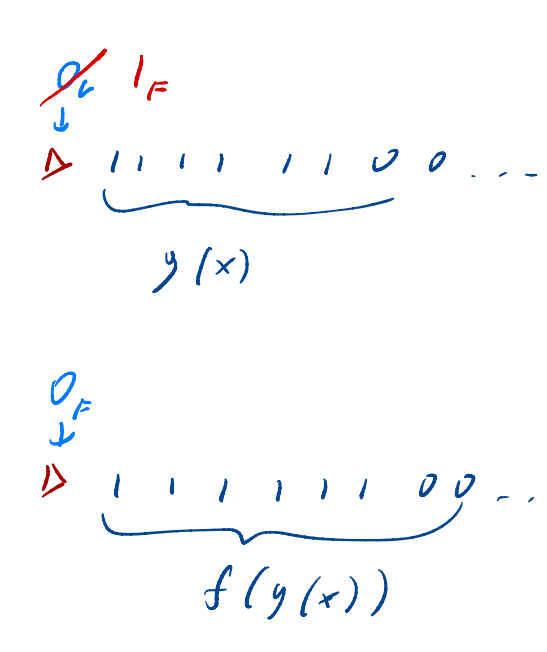
\includegraphics[width=\textwidth]{Immagini/composizione_di_TC_2.png}
    \end{minipage}
\end{figure}

Posso costruire per bene una macchina $H$ che implementa le operazioni fatte a mano.

\begin{proof}
    Supponiamo per comodità che $\Sigma_G = \Sigma_F = \{0,1,\blacktriangleright\} =: \Sigma_H$, definiamo $Q_H := Q_G \sqcup Q_F$, dove poniamo $1_H := 1_G$ e $0_H := 0_F$ - rispettivamente stato iniziale della macchina $H$ 
    e stato finale della macchina $H$. Per la funzione di transizione definiamo:
    \[ \delta_H : Q_H \times \Sigma_H \to Q_H \times \Sigma_H \times \{\leftarrow, \downarrow, \rightarrow\} : \delta_H(q,\sigma) := \begin{cases}
                                                                                                                                     \delta_G(q,\sigma) & \text{se $q \in Q_G\setminus\{0_G\}$} \\
                                                                                                                                     \delta_F(1_F,\sigma) & \text{se $q = 0_G$} \\
                                                                                                                                     \delta_F(q,\sigma) & \text{se $q \in Q_F$}
    \end{cases}\]
    cioè se sono nello stato finale di $G$, mi comporto come se fossi in quello iniziale di $F$ - questo corrisponderebbe al nostro intervento manuale, altrimenti mi comporto come la macchina dello stato a cui appartengo.                                                                                 
\end{proof}

Ora si pone il problema di generalizzare questo argomento alla composizione arbitraria. Costruiamo delle macchine che calcolino $f$, ma con qualche vincolo in più
rispetto a quelli richiesti dalla definizione di Turing-computabilità, questa scelta è sia comoda che possibile, per cui la adottiamo. Data $f$ vogliamo costruire la
tabella delle funzioni di transizione della macchina che calcola $f$, lo facciamo a pezzi, cioè prendiamo dei sottoinsiemi degli stati e scriviamo dove vanno.\\

\textbf{Setting}: L'alfabeto per la costruzione di queste macchine sarà costituito solo dai tre simboli di base per la Turing-computabilità, ovvero $\Sigma = \{0,1,\blacktriangleright\}$, per cui definiremo solo nuovi stati.

\begin{notation}[Notazione per descrivere il comportamento di pezzi di TM]
    Con la notazione: $s_1 \to \texttt{macchina} \to s_2$ intendiamo che, preso un sottoinsieme di stati, dove $s_1$ è lo stato iniziale, che prendiamo sopra a $\blacktriangleright$, seguito da una configurazione
    \begin{figure}[H]
        \centering
        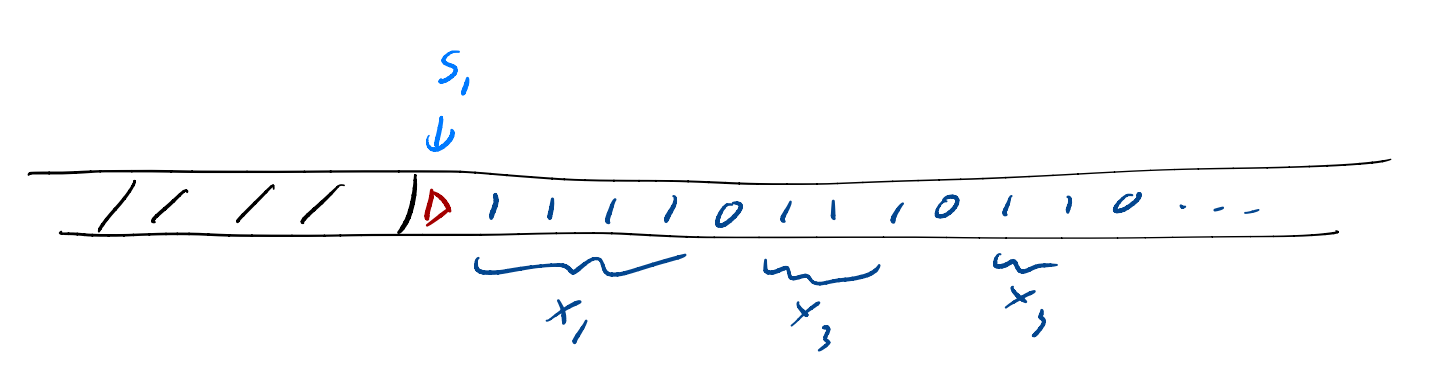
\includegraphics[width=0.6\textwidth]{Immagini/notazione_macchina_1.png}
    \end{figure}
    o non ritorna mai nello stato $s_2$, o ritorna, nello stato $s_2$, sul $\blacktriangleright$, in una nuova configurazione. Assumiamo inoltre che le macchine che stiamo costruendo non vadano mai a sinistra di $\blacktriangleright$.
    \begin{figure}[H]
        \centering
        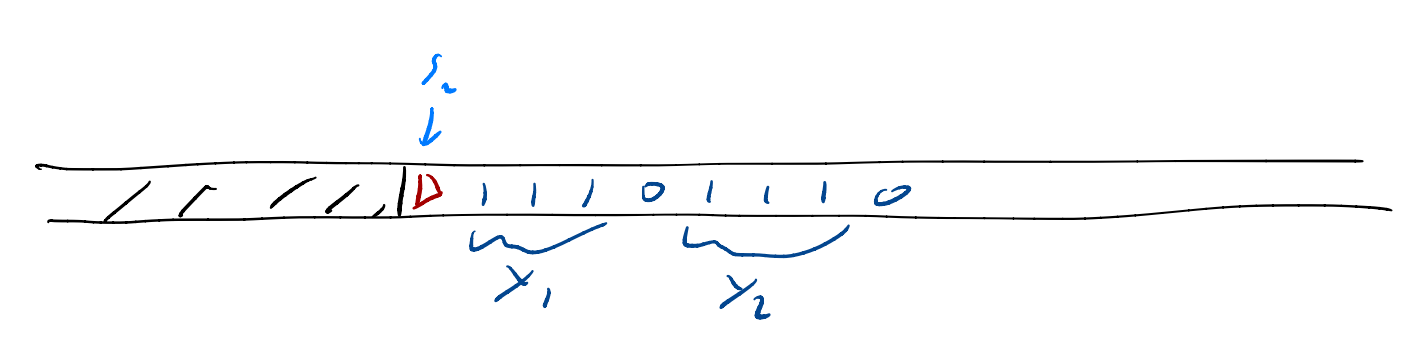
\includegraphics[width=0.6\textwidth]{Immagini/notazione_macchina_2.png}
    \end{figure}
    Quindi $s_1 \to \texttt{macchina} \to s_2 \overset{\text{def}}{\iff}$ la $\texttt{macchina}$ viene posta nello stato $s_1$ sopra a $\blacktriangleright$, con la configurazione - sempre scritta in notazione unaria con gli 0 - che sarà indicata tra parentesi,
    allora, senza mai toccare ciò che sta a sinistra del triangolino, porta la macchina nello stato $s_2$ sopra a $\blacktriangleright$, con una nuova configurazione - nella solita notazione - che sarà indicata tra parentesi, oppure non termina mai:
    \[ s_1 \to \texttt{macchina} \to s_2(s_1 \blacktriangleright x_1 x_2 \ldots x_k \ldots) = s_2 \blacktriangleright y_1 y_2 \ldots \]
\end{notation}

Quindi con questa notazione possiamo facilmente descrivere il comportamento di pezzi di macchine, e poi comporli per ottenere macchine più complesse.

\begin{definition}[Macchine elementari]
    Definiamo le seguenti macchine elementari:
    \begin{itemize}
        \item $\textcolor{purple}{s_1 \to \push_{n,i} s_2}(s_1 \blacktriangleright x_1 x_2 \ldots x_n) = s_2 \blacktriangleright x_1 x_2 \ldots x_n x_i$, dove la nuova configurazione ha $n+1$ numeri, ha copiato l'$i$-esimo numero in fondo alla fila;
        \item $\textcolor{purple}{s_1 \to \rem_{n,i} s_2}(s_1 \blacktriangleright x_1 x_2 \ldots x_n) = s_2 \blacktriangleright x_1 x_2 \ldots x_{i-1} x_{i+1} \ldots x_n$, dove la nuova configurazione ha $n-1$ numeri, ha rimosso l'$i$-esimo numero;
        \item $\textcolor{purple}{s_1 \to \exec_{n,k}f s_2}(s_1 \blacktriangleright x_1 x_2 \ldots x_n) = s_2 \blacktriangleright x_1 x_2 \ldots x_{n-k} f(x_{n-k+1}, \ldots, x_n)$, dove la nuova configurazione ha $n-k+1$ numeri, ha eseguito la funzione $f$ sugli ultimi $k$ numeri, e ha aggiunto il risultato in fondo alla fila;
        \item infine definiamo la macchina che controlla che l'$i$-esimo numero sia 0:
        \[ \textcolor{purple}{s_1 \to \ttif x_i = 0 \to s_2\lor s_3}(s_1 \blacktriangleright x_1 x_2 \ldots x_n) = \begin{cases}
            s_2 \blacktriangleright x_1 x_2 \ldots x_n & \text{se $x_i = 0$} \\
            s_3 \blacktriangleright x_1 x_2 \ldots x_n & \text{se $x_i \ne 0$} 
        \end{cases} \]
        i simboli sono uguali, cambia solo lo stato in cui si ritrova la macchina su $\blacktriangleright$, in base a se $x_i$ è 0 o no.
    \end{itemize}
\end{definition}

Adesso il piano è: assumiamo di avere queste macchine elementari, e dimostriamo che la classe delle funzioni Turing-computabili, rappresentabili mediante
macchine di Turing che hanno come alfabeto $\Sigma = \{0,1,\blacktriangleright\}$ e che non vanno mai a sinistra di $\blacktriangleright$, è chiusa per composizione, ricorsione primitiva e minimizzazione.
Dobbiamo anche definire macchine di Turing che implementino le funzioni: successore, sottrazione troncata per 1, costante 0 e proiezione. Infine vediamo come implementare le macchine elementari e con questo abbiamo dimostrato che ogni funzione ricorsiva è Turing-computabile.

\begin{proof}
    Vediamo che la classe delle funzioni Turing-computabili è chiusa per composizione, ricorsione primitiva e minimizzazione. In tutti i casi faremo la seguente cosa: assumiamo di avere le macchine elementari che implementano le operazioni di \texttt{push}, \texttt{rem}, \texttt{exec}, \texttt{ttif} e vediamo come usarle per costruire macchine che implementano le funzioni ottenute per composizione, ricorsione primitiva e minimizzazione.
    In particolare le nuove macchine saranno ottenute unendo gli stati - in maniera disgiunta per evitare problemi - e incollando le funzioni di transizione (come nell'esempio precedente), ci limiteremo pertanto a descrivere soltanto come sono fatte queste ultime, componendo quelle delle macchine elementari, e non descrivendo per intero le funzioni implementate da queste macchine.
    \begin{itemize}
        \item[$\boxed{\text{composizione}}$] Se $f : \NN^k \to \NN_\bot$ e $g_1, \dots, g_k : \NN^h \to \NN_\bot$, vogliamo costruire una macchina che parta da $\blacktriangleright x_1 \ldots x_h$ e arrivi a $\blacktriangleright f(g_1(x_1, \dots, x_h), \dots, g_k(x_1, \dots, x_h))$.\\
        Iniziamo copiando tutti gli input in fondo alla lista:
        \[ \footnote{Per comodità, d'ora in poi chiameremo gli stati solo con i numeri.}1 \to \push_{h,1} \to \push_{h+1,2} \to \ldots \to \push_{2h-1,h} \to 2 \]
        con $2 \blacktriangleright x_1 \ldots x_h x_1 \ldots x_h$. Ora usiamo $\exec_{2h,h}g_1$ per calcolare $g_1$:
        \[ 2 \to \exec_{2h,h}g_1 \to 3 \]
        con $3 \blacktriangleright x_1 \ldots x_h g_1(x_1, \dots, x_h)$. Ripetendo queste operazioni $k$ volte, e otteniamo lo stato $4 \blacktriangleright x_1 \ldots x_h g_1(x_1, \dots, x_h) \ldots g_k(x_1, \dots, x_h)$. A questo punto cancelliamo i primi $h$ numeri e calcoliamo $f$:
        \[ 4 \to \rem_{h+k,1} \to \rem_{h+k-1,1} \to \ldots \to \rem_{k+1,1} \to \exec_{k,k}f \to 5 \]
        con $5 \blacktriangleright f(g_1(x_1, \dots, x_h), \dots, g_k(x_1, \dots, x_h))$, infine vado da $5$ a $0$ per stoppare la macchina. Restano i casi in cui $g_i(x_1, \dots, x_h) = \bot$ per qualche $i$, oppure $f(g_1(x_1, \dots, x_h), \dots, g_k(x_1, \dots, x_h)) = \bot$,
        in ambo i casi, per ipotesi, le macchine che implementano $g_i$ o $f$ non terminano, e quindi anche $\exec\, g_i$ o $\exec\, f$ non termina, per cui la macchina che abbiamo costruito non termina, e quindi è coerente con $f(g_1(x_1, \dots, x_h), \dots, g_k(x_1, \dots, x_h)) = \bot$.
        \item[$\boxed{\text{ricorsione primitiva}}$] Siano $h : \NN^k \to \NN_\bot$ e $g : \NN^{k+2} \to \NN_\bot$, Turing computabili, e vogliamo implementare $f : \NN^{k+1} \to \NN_\bot$, definita via ricorsione primitiva a partire da $h$ e $g$:
        \[ f(x,y_1,\dots,y_k) := \begin{cases}
            f(0, y_1, \dots, y_k) := h(y_1, \dots, y_k) \\
            f(x + 1, y_1, \dots, y_k) := g(x, f(x, y_1, \dots, y_k), y_1, \dots, y_k)
        \end{cases} \]
        Calcoliamo al contrario la ricorsione, e teniamoci un contatore in modo da sapere quando fermarci. Assumiamo, WLOG, di avere uno 0 alla fine della stringa di input,
        ovvero $1 \blacktriangleright x y_1 \ldots y_k 0$, calcoliamo $f(0, y_1, \dots, y_k) = h(y_1, \dots, y_k)$:
        \[ 1 \to \push_{k+2,2} \to \push_{k+3,3} \to \ldots \to \push_{2k+1,k+1} \to \exec_{2k+2,k}h \to 2 \]
        con $2 \blacktriangleright x y_1 \ldots y_k 0 h(y_1, \dots, y_k)$, ora controlliamo se siamo nel caso base o no:
        \[ 2 \to \ttif x = 0 \to \begin{cases}
            3 & \text{se $x = 0$} \\
            4 & \text{se $x \ne 0$}
        \end{cases} \]
        per cui $3 \blacktriangleright 0 y_1 \ldots y_k 0 h(y_1, \dots, y_k)$, e siamo arrivati in questo caso, è sufficiente applicare $k+2$ volte $\rem$ e poi andare a $0$ per ottenere $0 \blacktriangleright f(0, y_1, \dots, y_k)$.\\
        Prima di procedere con 4, dimostriamo un lemma.
        \begin{lemma}
            Dalla configurazione:
            \[ \blacktriangleright x - t y_1 \ldots y_k t f(t, y_1, \dots, y_k) \]
            e $t \in \NN$, si può passare alla configurazione, in un altro stato:
            \[ \blacktriangleright x - (t+1) y_1 \ldots y_k (t+1) f(t+1, y_1, \dots, y_k) \]
        \end{lemma}
        Una volta dimostrato questo lemma, avremo dimostrato per induzione - il caso base è quello sopra - che se $x - t \ne 0$, allora possiamo passare alla configurazione con $t+1$;
        fatto questo si applica $\ttif x - (t+1) = 0$ per verificare se siamo arrivati allo stato 3, ed in tal caso, a meno di cancellare i primi simboli abbiamo concluso.
        Altrimenti si continua, in un altro stato, col passo ricorsivo, per cui da 4 si continua per $x$ passi, e poi si arriva alla terminazione,
        e questo accade necessariamente perché $x \in \NN$ e $x - t = 0$ per $t$ sufficientemente grande.
        \begin{proof}
            Chiamiamo $a$ lo stato iniziale, allora, in primis ricopiamo in fondo $x-t$ e sottraiamo 1:
            \[ a \to \push_{k+3,1} \to \exec_{k+4,1}\dotminus 1 \to b \]
            con $b \blacktriangleright x - t y_1 \ldots y_k t f(t, y_1, \dots, y_k) x - (t+1)$, copiamo ora gli input $y_1,\dots,y_k$ in fondo:
            \[ b \to \push_{k+4,2} \to \push_{k+5,3} \to \ldots \to \push_{2k+3,k+1} \to c \]
            con $c \blacktriangleright x - t y_1 \ldots y_k t f(t, y_1, \dots, y_k) x - (t + 1) y_1 \ldots y_k$, ora copiamo in fondo gli argomenti necessari per il passo ricorsivo, cioè $t$, $f(t,y_1,\dots,y_k)$ e $y_1,\dots,y_k$, e poi applichiamo $g$:
            \begin{multline*}
                c \to \push_{2k+3,k+2} \to \push_{2k+4,k+3} \to \\ \to \push_{2k+5,2} \to \ldots \to \push_{3k+4,k+1} \to \exec_{3k+5,k+2}g \to d
            \end{multline*}
            Cancellando con $\rem$ tutti i simboli iniziali otteniamo $\blacktriangleright x - (t + 1) y_1 \ldots y_k (t+1) f(t+1, y_1, \dots, y_k)$, e da qui si arriva allo stato terminale.\\
        \end{proof}
        Rimane il caso in cui $h(y_1, \dots, y_k) = \bot$ o $g(i, f(x, y_1, \dots, y_k), y_1, \dots, y_k) = \bot$, per qualche $i \leq x$, in tal caso, per ipotesi, le macchine associate a $h$ e $g$ non terminano e di conseguenza non terminano $\exec\, h$ o $\exec\, g$,
        per cui non termina la macchina che implementa $f$, coerentemente col fatto che $f(x,y_1,\dots,y_k) = \bot$ come funzione ricorsiva.
        \item[$\boxed{\text{minimizzazione}}$] Sia $g : \NN^{k+1} \to \NN_\bot$ Turing computabile, e vogliamo implementare $f : \NN^k \to \NN_\bot$, definita via minimizzazione a partire da $g$:
        \[ f(y_1, \dots, y_k) := \mu_x g(x, y_1, \dots, y_k) \]
        Partiamo da $1 \blacktriangleright 0 y_1 \ldots y_k$, dove usiamo lo 0 come base del contatore che ci serve.
        Dimostriamo che, partendo dallo stato $2 \blacktriangleright t y_1 \ldots y_k$, con $t \in \NN$, o si ottiene l'output voluto, oppure si ritorna nello stesso stato ma con $t+1$.
        Copiamo in fondo i valori $t,y_1,\dots,y_k$ e calcoliamo $g(t,y_1,\dots,y_k)$:
        \[2 \to \push_{k+1,1} \to \push_{k+2,2} \to \ldots \to \push_{2k+1,k+1} \to \exec_{2k+2,k+1}g \to 3\]
        con $3 \blacktriangleright t y_1 \ldots y_k g(t,y_1,\dots,y_k)$, ora controlliamo se $g(t,y_1,\dots,y_k) = 0$:
        \[ 3 \to \ttif x_{k+2} = 0 \to \begin{cases}
            4 & \text{se $g(t,y_1,\dots,y_k) = 0$} \\
            5 & \text{se $g(t,y_1,\dots,y_k) \ne 0$}
        \end{cases} \]
        da 4 è sufficiente cancellare i simboli iniziali e andare a $0$ per concludere. Nel ramo 5, invece, cancelliamo $g(t,y_1,\dots,y_k)$ e torniamo a 2:
        \begin{multline*}
            5 \to \rem_{k+2,k+2} \to \push_{k+1,1} \to \exec_{k+2,1}+1 \to \push_{k+2,2} \to \\ \to \push_{k+3,3} \to \ldots \to \push_{2k+1,k+1} \to \rem_{2k+2,1} \to \rem_{2k+1,1} \to \\ \to \ldots \to \rem_{k+2,1} \to 2
        \end{multline*}
        Quindi la macchina termina esattamente quando trova il minimo $a$ tale che $g(a,y_1,\dots,y_k)=0$.
        Se non esiste $i$ tale che la computazione di $g(i,y_1,\dots,y_k)$ termina, oppure se $g(i,y_1,\dots,y_k) = \bot$ per qualche $i$ prima di trovare un valore zero, allora la macchina non raggiunge mai lo stato $0$,
        e questo è coerente con la definizione di quando si ha $f(y_1,\dots,y_k)=\bot$ per minimizzazione.
    \end{itemize}
\end{proof}

Rimane ora da costruire le macchine elementari, e le macchine che implementano le funzioni $s$, $0_k$, $\pi_{k,i}$ e $\dotminus 1$.

\enlargethispage{1\baselineskip}

\begin{remark}[TM che implementano $\pi_{k,i}$ e $0_k$]
    Osservare che $\pi_{k,i}$ è implementabile con una sequenza di $\rem$ che cancella tutti i numeri tranne l'$i$-esimo, ricordando che lavoriamo in notazione unaria si lascia solo il blocco di uni relativo all'$i$-esimo numero;
    $0_k$ è implementabile semplicemente prendendo la rappresentazione in notazione unaria dei $k$ numeri, e cancellando tutto fino a lasciare solo $\blacktriangleright 00\ldots$, che rappresenta correttamente lo 0 in notazione unaria.
\end{remark}

\begin{exercise}
    Costruire macchine di Turing che implementino le funzioni $s$ e $\dotminus 1$.
\end{exercise}

\begin{soln}
    Per implementare $s$, partendo da $1 \blacktriangleright 1\ldots1$, con $x$ simboli 1, basta aggiungere un altro simbolo 1 alla fine della stringa, per cui possiamo definire la funzione di transizione della macchina di Turing come segue:
    \begin{table}[H]
    \centering
    \begin{tabular}{c|ccc}
        & $\blacktriangleright$ & $0$ & $1$ \\ \hline
        $0$   & $0$ $\blacktriangleright$ $\downarrow$    & $0$ $0$ $\downarrow$    & $0$ $1$ $\downarrow$ \\ 
        $1$   & $1$ $\blacktriangleright$ $\rightarrow$   & $2$ $1$ $\downarrow$   & $1$ $1$ $\rightarrow$ \\
        $2$   & $0$ $\blacktriangleright$ $\downarrow$   & $2$ $0$ $\leftarrow$    & $2$ $1$ $\leftarrow$ \\
    \end{tabular}
    \end{table}
    Prendendo $\Sigma = \{0,1,\blacktriangleright\}$ e $Q = \{0,1,2\}$, abbiamo definito la macchina che implementa la funzione successore $s$.\\
    Per implementare $\dotminus 1$, partendo da $1 \blacktriangleright 1\ldots1$, con $x$ simboli 1, basta cancellare l'ultimo simbolo 1 della stringa, per cui possiamo definire:
    \begin{table}[H]
    \centering
    \begin{tabular}{c|ccc}
        & $\blacktriangleright$ & $0$ & $1$ \\ \hline
        $0$   & $0$ $\blacktriangleright$ $\downarrow$    & $0$ $0$ $\downarrow$    & $0$ $1$ $\downarrow$ \\ 
        $1$   & $1$ $\blacktriangleright$ $\rightarrow$   & $2$ $0$ $\leftarrow$   & $1$ $1$ $\rightarrow$ \\
        $2$   & $0$ $\blacktriangleright$ $\downarrow$   & $2$ $0$ $\leftarrow$    & $3$ $0$ $\rightarrow$ \\
        $3$   & $0$ $\blacktriangleright$ $\downarrow$   & $3$ $0$ $\leftarrow$    & $3$ $1$ $\leftarrow$ \\
    \end{tabular}
    \end{table}
    Prendendo $\Sigma = \{0,1,\blacktriangleright\}$ e $Q = \{0,1,2,3\}$, abbiamo definito anche la macchina che implementa la funzione PR $\dotminus 1$.
\end{soln}

\begin{exercise}
    Costruire macchine di Turing che implementino le funzioni $\push$, $\rem$, $\exec$ e $\ttif$.
\end{exercise}

\begin{soln}
    Per tutte le macchine elementari usiamo $\Sigma = \{0,1,\blacktriangleright\}$ e $Q \supseteq \{0,1\}$.\\
    $\boxed{\ttif x_i = 0}$\\
    Vogliamo costruire una macchina che vada da $1 \blacktriangleright x_1 \ldots x_n$ a $2 \blacktriangleright x_1 \ldots x_n$ se $x_i = 0$, e a $3 \blacktriangleright x_1 \ldots x_n$ se $x_i \ne 0$.
    Quindi la tabella della funzione di transizione sarà composta da $4+i$ righe che mi servono per arrivare a $x_i$ e poi decidere se andare in 2 o 3, da cui $Q = \{0,1,2,3,\alpha_1,\ldots,\alpha_i\}$ e:
    \begin{table}[H]
    \centering
    \begin{tabular}{c|ccc}
        & $\blacktriangleright$ & $0$ & $1$ \\ \hline
        $0$   & $0$ $\blacktriangleright$ $\downarrow$    & $0$ $0$ $\downarrow$    & $0$ $1$ $\downarrow$ \\ 
        $1$   & $\alpha_1$ $\blacktriangleright$ $\rightarrow$   & $\alpha_1$ $0$ $\rightarrow$   & $\alpha_1$ $1$ $\rightarrow$ \\
        $\alpha_j$ ($1 \leq j \leq i-1$)  & $\alpha_j$ $\blacktriangleright$ $\rightarrow$    & $\alpha_{j+1}$ $0$ $\rightarrow$  & $\alpha_j$ $1$ $\rightarrow$ \\
        $\alpha_i$ & $\alpha_i$ $\blacktriangleright$ $\rightarrow$    & $2$ $0$ $\rightarrow$   & $3$ $1$ $\rightarrow$ \\
        $2$   & $2$ $\blacktriangleright$ $\downarrow$   & $2$ $0$ $\leftarrow$    & $2$ $1$ $\leftarrow$ \\
        $3$   & $3$ $\blacktriangleright$ $\downarrow$    & $3$ $0$ $\leftarrow$    & $3$ $1$ $\leftarrow$
    \end{tabular}
    \end{table}
    avendo definito $\Sigma, Q$ e $\delta$, abbiamo costruito la macchina che implementa $\ttif x_i = 0$.\\
    $\boxed{\rem_{n,i}}$ e $\boxed{\push_{n,i}}$\\
    Non sono semplicissime da implementare usando solo $\Sigma = \{0,1,\blacktriangleright\}$, e per far funzionare tutto il resto ci conviene restare solo con questi simboli,
    pertanto non le riporto, in ogni caso $\push_{n,i}$ è più semplice da implementare, mentre $\rem_{n,i}$ è più complicata.\\
    $\boxed{\exec_{n,k} f}$\\
    Vogliamo costruire una TM che parta da $1 \blacktriangleright x_1 \ldots x_n$ e arrivi alla configurazione $0 \blacktriangleright x_1 \ldots x_{n-k} f(x_{n-k+1}, \ldots, x_n)$.
    Trattiamo qui il caso $1 \leq k < n$ (se $k = n$, si applica direttamente la macchina $F$ all'intero input).
    Sia $F$ la macchina di Turing che implementa $f$. La configurazione iniziale corrisponde sul nastro a:
    \[ \blacktriangleright \underbrace{11\ldots 11}_{x_1} 0 \underbrace{11\ldots 11}_{x_2} 0 \ldots 0 \underbrace{11\ldots 11}_{x_{n-k}} 0 \underbrace{11\ldots 11}_{x_{n-k+1}} 0 \ldots 0 \underbrace{11\ldots 11}_{x_n} 00\ldots \]
    in primis vogliamo che la macchina si sposti verso destra fino a raggiungere $x_{n-k+1}$; arrivati allo 0 prima di $x_{n-k+1}$, ci mettiamo $\blacktriangleright$,
    a questo punto si usa che la TM che implementa $f$ non va mai a sinistra di $\blacktriangleright$. Fatto questo abbiamo $f(x_{n-k+1}, \ldots, x_n)$, per cui bisogna solo tornare indietro,
    la tabella della funzione di transizione sarà:
    \begin{table}[H]
    \centering
    \begin{tabular}{c|ccc}
        & $\blacktriangleright$ & $0$ & $1$ \\ \hline
        $0$ & $0$ $\blacktriangleright$ $\downarrow$ & $0$ $0$ $\downarrow$ & $0$ $1$ $\downarrow$ \\
        $1$ & $\alpha_1$ $\blacktriangleright$ $\rightarrow$ & $\alpha_1$ $0$ $\rightarrow$ & $\alpha_1$ $1$ $\rightarrow$ \\
        $\alpha_j$ ($1 \leq j \leq n-k-1$) & $\alpha_j$ $\blacktriangleright$ $\rightarrow$ & $\alpha_{j+1}$ $0$ $\rightarrow$ & $\alpha_j$ $1$ $\rightarrow$ \\
        $\alpha_{n-k}$ & $\alpha_{n-k}$ $\blacktriangleright$ $\rightarrow$ & $1_F$ $\blacktriangleright$ $\downarrow$ & $\alpha_{n-k}$ $1$ $\rightarrow$ \\
        \hline
        \multicolumn{4}{c}{tabella di $F \setminus \{0_F\}$} \\
        \hline
        $0_F$ & $2$ $0$ $\leftarrow$ & $2$ $0$ $\leftarrow$ & $2$ $1$ $\leftarrow$ \\
        $2$ & $0$ $\blacktriangleright$ $\downarrow$ & $2$ $0$ $\leftarrow$ & $2$ $1$ $\leftarrow$
    \end{tabular}
    \end{table}
\end{soln}

Occupiamoci ora di dimostrare che se $f$ è Turing-computabile, allora $f$ è ricorsiva, vedremo una cosa più forte, ovvero che \textcolor{MidnightBlue}{esiste una funzione ricorsiva che simula ogni funzione Turing-computabile}.

\begin{remark}
    Ricordando le definizioni di $\car$ e $\cdr$, come rispettivamente inversa sulla prima e sulla seconda componente di $\cons$,
    essendo $\cons : \NN^2 \hookrightarrow \NN\setminus\{0\}$, possiamo estendere le definizioni di $\car$ e $\cdr$ in 0, ponendo $\car(0) = \cdr(0) = 0$.
\end{remark}

\begin{definition}[Codifica di una lista]
    Definiamo $\langle a_1,\ldots,a_n \rangle$, una \vocab{codifica di una lista} di numeri naturali, come il numero:
    \[ \cons(a_1, \cons(a_2, \ldots \cons(a_{n}, \textcolor{purple}{0})\ldots))\]
    ovvero codifichiamo una sequenza di numeri in un numero utilizzando la funzione $\cons$ iterata.
    Alternativamente, se ne può dare una definizione ricorsiva:
    \begin{itemize}
        \item $\langle \rangle := 0$,
        \item $\langle a_1, \ldots, a_n \rangle := \cons(a_1, \langle a_2, \ldots, a_n \rangle)$.
    \end{itemize}
    - questa è compatibile con la prima definizione, poiché $\langle a \rangle = \cons(a, \langle \rangle) = \cons(a, 0)$.
\end{definition}

\begin{remark}[Iniettività della codifica di una lista]
    Tale codifica è iniettiva, e si verifica per induzione e usando che $\cons$ è iniettiva.
\end{remark}

\begin{example}
    La lista $\langle 7,15,0,9 \rangle$ viene codificata come $\cons(7, \cons(15, \cons(0, \cons(9,\textcolor{purple}{0}))))$.
    \begin{figure}[H]
        \centering
        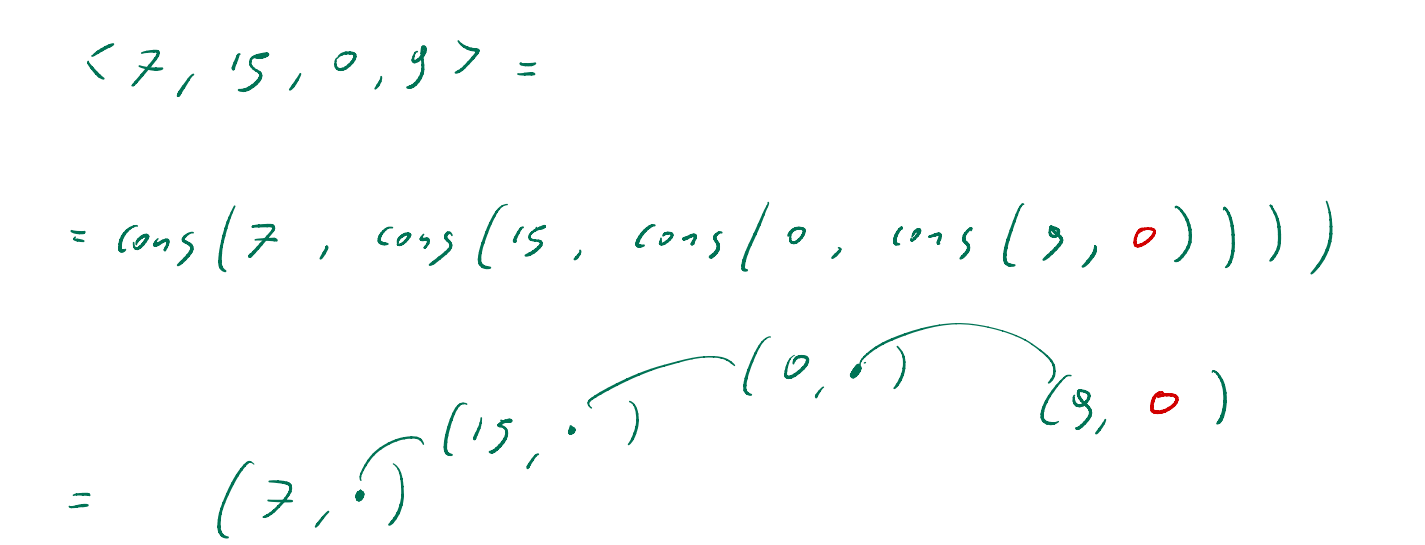
\includegraphics[width=0.7\textwidth]{Immagini/codifica_liste.png}
    \end{figure}
\end{example}

\begin{definition}[Funzioni sulle liste]
    Definiamo le seguenti funzioni PR sulle liste:
    \begin{itemize}
        \item $\nth(\langle a_0, \ldots, a_n \rangle, k) := a_k$ se $k \leq n$, e 0 altrimenti,
        \item $\length(\langle a_0, \ldots, a_n \rangle) := n+1$,
        \item $\cat(\langle a_0, \ldots, a_m \rangle, \langle b_0, \ldots, b_n \rangle) := \langle a_0, \ldots, a_m, b_0, \ldots, b_n \rangle$,
        \item $\head(\langle a_0, \ldots, a_n \rangle,k) := \langle a_0, \ldots, a_{k-1} \rangle$ se $k \leq n+1$, e $\langle a_0, \ldots, a_n \rangle$ altrimenti,
    \end{itemize}
\end{definition}

\begin{exercise}[Le funzioni sulle liste sono PR]
    Verificare che le funzioni $\nth$, $\length$, $\cat$ e $\head$ sono PR.
\end{exercise}

\begin{soln}
    Vediamo ora solo il caso di $\nth$, $\length$ e $\cat$. Per $\nth$ l'idea è che $\nth(\cdot,k) = \car \circ \cdr^k$, tuttavia, non essendo $k$ fissato a priori, non è immediato che la composizione sia PR,
    per tale ragione introduciamo una funzione ausiliaria $g(l,k)$ che coincide con $\cdr^k$, ed è PR in quanto definita per ricorsione primitiva via funzioni PR:
    \[ g(l,k) := \begin{cases}
        g(l,0) := l \\
        g(l,k+1) := \cdr(g(l,k))
    \end{cases} \]
    ora $g(l,k)$ coincide con $\cdr^k$, infatti il passo ricorsivo fatto $k$ volte corrisponde a $\cdr^k$; 
    inoltre $\boxed{\nth(l,k) = \car \circ g(l,k)}$, infatti, se $l = \langle a_0, \ldots, a_n \rangle$, allora $g(l,k) = \langle a_k, \ldots, a_n \rangle$, e prendendo $\car$ si ottiene $a_k$ se $k \leq n$;
    mentre se $k>n$, allora $g(l,k)=0$, in quanto arriviamo con $\cdr$ a 0 e $\car(0)=0$.\\
    Per $\length$ basterà osservare che $\boxed{\length(l) = \#\{i < l| \cdr^i(l) \ne 0\}}$, cioè quante volte si può fare $\cdr$ prima di arrivare a 0;
    tale funzione è PR, perché per ogni $i \in \NN$ $\{\cdr^i(l) \ne 0\}$ è un predicato PR, e $l \mapsto \#\{i < l| \cdr^i(l) \ne 0\}$ è una funzione che conta gli elementi di un predicato PR fino a $l$, che è quindi PR per un esempio precedente.
    Infine è facile osservare che $n+1 = \length(l)$ se e solo se $\cdr^{n+1}(l) = 0$ - sto indicizzando da $a_0$, quindi il numero di applicazioni di $\cdr$ necessarie per arrivare a 0 coincide con la lunghezza della lista - da cui la definizione di $\length$ data sopra funziona.\\
    Per $\cat$ è sufficiente mettere la seconda codifica più interna e poi aggiungere in testa gli elementi della prima lista partendo dall'ultimo, così da preservarne l'ordine finale; questo può essere fatto definendo la seguente funzione PR:
    \[ f(a,b,k) := \begin{cases}
        f(a,b,0) := b \\
        f(a,b,k+1) := \cons(\nth(a,\length(a)\dotminus(k+1)), f(a,b,k))
    \end{cases} \]
    in pratica per calcolare $f(a,b,k)$ si parte da $b$ e si aggiungono in testa prima l'ultimo elemento di $a$, poi il penultimo, e così via fino al primo; ne segue
    quindi che vale $\boxed{\cat(a,b) = f(a,b,\length(a))}$.
\end{soln}

Per dimostrare che anche $\head$ è PR ci serve un lemma.

\begin{lemma}[Ricorsione sul (de)corso dei valori]
    Sia $f : \NN^{n+1} \to \NN$ una funzione e $g : \NN^{n+1} \to \NN$ PR, tali che:
    \[ f(x_1, \ldots, x_n,y) = g(x_1, \ldots, x_n, \langle f(\mathbf x,y-1), f(\mathbf x,y-2), \ldots, f(\mathbf x,0) \rangle) \]
    allora $f$ è PR.
\end{lemma}

\begin{proof}
    Sia $h(\mathbf{x},y) := \langle f(\mathbf x,y-1), \ldots, f(\mathbf x,0) \rangle$, se riusciamo a dimostrare che $h$ è PR, segue immediatamente che $f$ è PR per composizione.\\
    Per verificare che $h$ è PR, ne diamo una definizione per ricorsione primitiva:
    \[ h(\mathbf x,y) := \begin{cases}
        h(\mathbf x,0) = \langle \rangle = 0 \\
        h(\mathbf x,y+1) = \cons(g(\mathbf x, h(\mathbf x,y)), h(\mathbf x,y))
    \end{cases} \]
    dove abbiamo usato l'ipotesi per cui $f(\mathbf x,y) = g(\mathbf x, h(\mathbf x,y))$.
\end{proof}

\begin{example}[Successione di Fibonacci]
    Dal lemma precedente è facile dimostrare che la successione di Fibonacci $\texttt{fib}$ è PR, infatti:
    \[ \texttt{fib}(x) = g(\langle \texttt{fib}(x-1), \ldots, \texttt{fib}(0) \rangle) \]
    e possiamo definire $g$ per casi, sui predicati PR $\{\length(l) = 0\}$, $\{\length(l) = 1\}$ e $\{\length(l) > 1\}$, come segue:
    \[ g(l) := \begin{cases}
        0 & \text{se $\length(l) = 0$} \\
        1 & \text{se $\length(l) = 1$} \\
        \car(l) + \car(\cdr(l)) & \text{altrimenti}
    \end{cases} \]
\end{example}

A questo punto possiamo anche verificare che $\head$ è PR.

\begin{soln}
    \textcolor{MidnightBlue}{Per $\head$ potremmo dare la seguente definizione ricorsiva:
    \[ \head(l,k) := \begin{cases}
        \head(l,0) := 0 \\
        \head(l,k+1) := \cons(\car(l), \head(\cdr(l),k))
    \end{cases} \]
    che corrisponde all'idea di:
    \[ \langle \underbrace{a_0}_{\mathrlap{\mkern-23mu = \car(l)}}, \underbrace{a_1,\ldots,a_k}_{\mathrlap{\mkern-24mu =\head(\cdr(l),k)}},\ldots \rangle \]
    il problema è che nella ricorsione passo a $\head(\cdr(l),\ldots)$, anziché ad $\head(l,\ldots)$, per prendere la lista restante dopo aver preso il primo elemento, per cui non siamo in una ricorsione primitiva diretta su $k$ e quindi questo approccio non funziona.}\\ 
    Usiamo allora il lemma di ricorsione sul decorso dei valori e definiamo:
    \[ \boxed{\head(l,y)=g\left(l,\left\langle \head(l,y-1),\ldots,\head(l,0)\right\rangle\right)} \]
    dove $g$ è PR e vale
    \[ g(l,s):=\begin{cases}
        0 & \text{se }\length(s)=0\\
        \car(s) & \text{se }\length(s)>\length(l)\\
        \cat(\underbrace{\car(s)}_{\mathclap{\langle a_0,\ldots, a_{\length(s)\dotminus 1} \rangle}},\cons(\nth(l,\length(s)\dotminus 1),0)) & \text{altrimenti}
    \end{cases} \]
    infatti, se $s=\langle \head(l,y-1),\ldots,\head(l,0)\rangle$, allora $\car(s)=\head(l,y-1)$. Quando $\length(s)=0$ siamo nel caso base $y=0$, e quindi il valore corretto è $0$.
    Quando $\length(s)>\length(l)$ - ovvero se la lunghezza della lista dei valori supera la lunghezza della nostra lista - abbiamo già superato la lunghezza di $l$, perciò abbiamo già il prefisso richiesto e resta uguale all'ultimo valore calcolato nella lista $s$, cioè $\car(s)$.\\
    Nel caso rimanente, aggiungiamo a $\head(l,y-1)=\car(s)$ l'elemento successivo di $l$, cioè $\nth(l,\length(s)-1)$, e otteniamo esattamente $\head(l,y)$. 
    Quindi siamo esattamente nel caso del lemma, e $\head$ è PR.
\end{soln}

\begin{theorem}[Funzione ricorsiva universale]
    Esiste una funzione ricorsiva parziale $u : \NN_\bot^2 \to \NN_\bot$ tale che per ogni $f : \NN^k \to \NN_\bot$ Turing-computabile,
    esiste un numero $\ulcorner f \urcorner \in \NN$, detto \vocab{codice} di $f$, tale che:
    \[ \forall x_1, \ldots, x_k \in \NN \; f(x_1, \ldots, x_k) = u(\ulcorner f \urcorner, \langle x_1, \ldots, x_k \rangle) \]
    ovvero esiste una funzione universale $u$ che simula ogni funzione Turing-computabile, e le basta il codice della funzione e la codifica degli input.
\end{theorem}

\begin{corollary}[Turing-computabilità $\Rightarrow$ ricorsività]
    Se $f : \NN^k \to \NN_\bot$ è Turing-computabile, allora $f$ è ricorsiva.
\end{corollary}

\begin{proof}
    La dimostrazione segue dal teorema osservando che:
    \[ f(\cdot) = u(\ulcorner f \urcorner, \cdot) \]
    $u$ è ricorsiva dal teorema ed è composta con una costante.
\end{proof}

\begin{corollary}[Esistenza di una funzione ricorsiva universale per ogni arietà]
    $\forall n \in \NN \; \exists u_n : \NN_\bot^{n+1} \to \NN_\bot$ ricorsiva, tale che, data $f : \NN_\bot^n \to \NN_\bot$ ricorsiva,
    esiste un codice $\ulcorner f \urcorner$ tale che:
    \[ \forall x_1, \ldots, x_n \in \NN_\bot \; f(x_1, \ldots, x_n) = u_n(\ulcorner f \urcorner, x_1, \ldots, x_n) \]
\end{corollary}

\begin{proof}
    Dal teorema precedente, $f$ è ricorsiva, quindi Turing-computabile, per cui esiste $\ulcorner f \urcorner$ tale che $f(\cdot) = u(\ulcorner f \urcorner, \cdot)$,
    a questo punto è sufficiente definire $u_n$ come:
    \[ u_n(\ulcorner f \urcorner, x_1, \ldots, x_n) := u(\ulcorner f \urcorner, \langle x_1, \ldots, x_n \rangle) \]
    essendo la codifica una composizione di $n$ (con $n$ fisso) funzioni $\cons$, che è PR, $u_n$ è ricorsiva per composizione di funzioni ricorsive.
\end{proof}

\begin{remark}[Tesi di Church]
    ``La classe delle funzioni ricorsive coincide con la classe delle funzioni effettivamente calcolabili''. Tale tesi non è un'affermazione matematica,
    ma è l'idea che esprime la filosofia dietro alle varie nozioni di calcolabilità che abbiamo dato - e anche non dato, e.g. il $\lambda$-calcolo, che è quella di descrivere tutte le funzioni che 
    possono essere calcolate effettivamente nella realtà. La tesi di Church può essere espressa in maniera più forte o debole in base a quanto si richieda buona la corrispondenza 
    tra computabilità pratica e modello teorico, noi ci siamo limitati al risultato semantico - ovvero a quale sia il valore effettivo, ma si può dare anche una corrispondenza tenendo conto della
    complessità, ed a seconda di quanto uno richiede che la corrispondenza sia precisa viene una tesi più forte o debole.
\end{remark}

Passiamo alla dimostrazione del teorema.

\begin{proof}
    Sia $f : \NN^k \to \NN_\bot$ Turing-computabile - per ora la fissiamo ma a fine dimostrazione sarà noto come il calcolatore universale non dipenda dalla $f$ usata, e sia $M$ una macchina di Turing che implementa $f$. Per definizione sappiamo che $\{0,1,\blacktriangleright\} \subseteq \Sigma$ e 
    $\{0,1\} \subseteq Q$, inoltre, essendo entrambi insiemi finiti, possiamo assumere che $\Sigma, Q \subseteq \NN$ - assumiamo che $\blacktriangleright$ corrisponda a 2, ricordiamo infine che, per le nostre convenzioni, rappresentiamo $\{\leftarrow, \downarrow, \rightarrow\}$ come $\{0,1,2\}$.\\
    Ora codifichiamo con un numero naturale una configurazione e la funzione $\delta$ di transizione di $M$. Per la codifica di una configurazione usiamo semplicemente una lista:
    \[ \NN \ni \textcolor{purple}{\text{configurazione}} := \langle \text{stato, posizione, nastro} \rangle \]
    dove stato e posizione sono i numeri naturali stessi, mentre la funzione nastro, che va da $\NN$ a $\Sigma$, è codificata come una lista di numeri naturali, ovvero la configurazione $a_0a_1\ldots a_n 00\ldots$ corrisponde alla lista $\langle a_0, a_1, \ldots, a_n \rangle$.
    \begin{remark}[Non iniettività della codifica del nastro]
        Si osserva che la codifica della funzione nastro introdotta non è iniettiva, infatti $\langle a_0, a_1, \ldots, a_n \rangle$ codifica la 
        stessa configurazione di $\langle a_0, a_1, \ldots, a_n, 0 \rangle$ e così via, tuttavia questo non è un problema, in quanto non si perde alcuna informazione rispetto a quale sia la configurazione considerata.
    \end{remark}
    Per codificare la funzione di transizione $\delta$, associamo a tale funzione il numero $\ulcorner \delta \urcorner$ tale che:
    \[ \nth(\ulcorner \delta \urcorner, \langle \text{stato}, \text{simbolo} \rangle) = \langle \text{stato'}, \text{simbolo'}, \text{direzione} \rangle \]
    ovvero se penso $\ulcorner \delta \urcorner$ non come un numero, ma come la funzione da $\NN^2$ a $\NN^3$ dico che in ogni casella del suo dominio c'è la tripla immagina, questo però lo vedo in termini puramente di codifiche.
    Il fatto che $\ulcorner \delta \urcorner$ esista è garantito dal fatto che la funzione, insiemisticamente, è contenuta in un sottoinsieme finito di $\NN^5$ e quindi posso letteralmente considerare $m := \max\{\langle \text{stato}, \text{simbolo} \rangle\}$, chiamare
    $a_i := \langle \text{stato}', \text{simbolo}', \text{direzione} \rangle$ con $i = \langle \text{stato}, \text{simbolo} \rangle$, questo se $\delta$ manda effettivamente la configurazione corrispondente all'indice in quella corrispondente alla tripla, altrimenti $a_i := 0$,
    infine porre $\ulcorner \delta \urcorner := \langle a_0, \ldots, a_m \rangle$, quindi, semplicemente, listo gli output di $\delta$ indicizzati dagli input.\\
    \begin{remark}[Non iniettività della codifica di $\delta$]
        Per la stessa ragione di prima, la codifica $\ulcorner \delta \urcorner$ non è iniettiva.
    \end{remark}
    A questo punto abbiamo bisogno di una funzione che simuli uno step di $M$ a partire dalla codifica di una configurazione.
    \begin{lemma}[Funzione PR che simula uno step della TM]
        Esiste una funzione PR $\texttt{step} : \NN^2 \to \NN$, tale che mappa ogni codifica di configurazione $c$, vale:
        \[ c \overset{M}{\to} \texttt{step}(\ulcorner \delta \urcorner, c) \]
        ovvero $\texttt{step}$ è una funzione che, data la codifica di una configurazione e quella della funzione di transizione, restituisce la codifica della configurazione che si ottiene applicando uno step della macchina di Turing.
    \end{lemma}
    \begin{proof}
        Con la codifica data all'inizio abbiamo che:
        \begin{itemize}
            \item \textcolor{purple}{stato} $= \nth(c,0)$,
            \item \textcolor{purple}{posizione} $= \nth(c,1)$,
            \item \textcolor{purple}{nastro} $= \nth(c,2)$
        \end{itemize}
        ora il nastro è a sua volta la codifica di una lista:
        \[ \text{nastro} = \langle \underbrace{a_1,\ldots,a_{p-1}}_{=:\textcolor{MidnightBlue}{\alpha}}, \underbrace{a_p}_{=:\textcolor{MidnightBlue}{\sigma}}, \underbrace{a_{p+1},\ldots}_{=:\textcolor{MidnightBlue}{\beta}} \rangle \]
        dove:
        \begin{itemize}
            \item $\textcolor{MidnightBlue}{\alpha} := \head(\text{nastro},\text{posizione} \dotminus 1) = \langle a_1,\ldots,a_{p-1}\rangle = \head(\nth(c,2),\nth(c,1) \dotminus 1)$,
            \item $\textcolor{MidnightBlue}{\sigma} := \nth(\text{nastro},\text{posizione}) = a_p = \nth(\nth(c,2),\nth(c,1))$,
            \item $\textcolor{MidnightBlue}{\beta} := \cdr^{\text{posizione}}(\text{nastro}) = \langle a_{p+1},\ldots\rangle = \cdr^{\nth(c,1)}(\nth(c,2))$.
        \end{itemize}
        Quello che vogliamo fare è calcolare $\delta(\text{stato},\text{simbolo})$, ovvero $\nth(\ulcorner \delta \urcorner, \langle \text{stato}, \text{simbolo} \rangle) = \nth(\ulcorner \delta \urcorner, \langle \nth(c,0), \sigma \rangle)$,
        che dà la tripla codificata da $\langle \textcolor{MidnightBlue}{\text{stato}'}, \textcolor{MidnightBlue}{\text{simbolo}'}, \textcolor{MidnightBlue}{\text{direzione}} \rangle :=$\textcolor{purple}{\texttt{update}}. Da questo posso
        scrivere la configurazione di arrivo, infatti il nuovo nastro sarà:
        \[ \text{nastro}' := \cat(\alpha,\cons(\nth(\texttt{update,1}),\beta)) \]
        dove $\nth(\texttt{update,1})$ è simbolo$'$; il nuovo stato sarà $\nth(\texttt{update,0})$ e la nuova posizione sarà $(\text{posizione} + \nth(\texttt{update,2})) \dotminus 1$.
        Segue quindi che la nuova configurazione sarà codificata da:
        \[ \langle \nth(\texttt{update,0}), (\nth(c,1) + \nth(\texttt{update,2})) \dotminus 1, \cat(\alpha,\cons(\nth(\texttt{update,1}),\beta)) \rangle \]
        e chiamiamo questo numero $\texttt{step}(\ulcorner \delta \urcorner, c)$, ottenuto da una composizione di funzioni PR, per cui $\texttt{step}$ è PR.
    \end{proof}
    Ora, la funzione che itera uno step $(n,c,\ulcorner \delta \urcorner) \mapsto \texttt{step}^n(\ulcorner \delta \urcorner, c)$ è PR, la verifica si fa scrivendo la funzione via ricorsione primitiva.\\
    Da questa vogliamo scrivere la funzione che, in un certo numero di step, a partire da un certo input e dal codice di $f$, restituisce l'output.
    Definiamo una codifica dell'input:
    \[ \texttt{codifica\_input}(\langle x_1, \ldots, x_k \rangle) := \langle 1, 0, \cons(\blacktriangleright, \texttt{nastro}(\langle x_1, \ldots, x_k \rangle)) \rangle \]
    dove:
    \[ \texttt{nastro}(\langle x_1, \ldots, x_k \rangle) := \cat(\texttt{unario}(x_1),\cons(0,\texttt{nastro}(\langle x_2, \ldots, x_k \rangle))) \]
    e $\texttt{unario}(x) := \langle 1, \ldots, 1 \rangle$ è la codifica unaria di $x$, tutte queste cose sono PR per composizione di funzioni PR.\\
    A questo punto usiamo l'operatore di minimizzazione per procurarci l'$n$ in cui la macchina termina, consideriamo:
    \[ \texttt{n}(c, \ulcorner \delta \urcorner) := \mu_n(\nth(\texttt{step}^n(\ulcorner \delta \urcorner, c) , 0)) \]
    ovvero $\texttt{n}$ rappresenta il numero di passi in cui la TM arriva allo stato 0 - termina - a partire da input codificato da $c$; tale funzione non è PR in quanto, per un certo input, la macchina potrebbe non terminare, per cui $\texttt n$ è \textbf{ricorsiva parziale}. E siamo alla fine perché ora per 
    ottenere l'output basta prendere il nastro della configurazione finale, ovvero, indicando con $\langle\mathbf{x}\rangle = \langle x_1, \ldots, x_k \rangle$:
    \[ \nth(\texttt{step}^{\texttt{n}(\texttt{codifica\_input}(\langle\mathbf{x}\rangle),\ulcorner \delta \urcorner)}(\ulcorner \delta \urcorner, \texttt{codifica\_input}(\langle\mathbf{x}\rangle))), 2) \]
    a questo punto prendo il nastro della configurazione finale e ci applico una funzione che conta gli 1, che darà proprio l'output di $f$ - a meno di sottrarre 2 perché abbiamo detto all'inizio che $\blacktriangleright$ corrisponde a 2, posso definire:
    \[ \texttt{conta\_uni}(l) := \begin{cases}
        0 & \text{se } \car(l) = 0 \\
        1 + \texttt{conta\_uni}(\cdr(l)) & \text{altrimenti}
    \end{cases}\]
    e quindi $u$ si definisce componendo $\texttt{conta\_uni}$ con la funzione scritta sopra, tale composizione, eccetto per la $\texttt n$, che fa uso di minimizzazione, è PR, per cui la composizione è ricorsiva parziale.
\end{proof}

\begin{corollary}[Forma normale per le funzioni ricorsive]
    $\forall k \in \NN$ esiste $T_k : \NN^{k+2} \to \NN$ predicato PR, e una funzione $U : \NN \to \NN$ PR, tali che
    $\forall f : \NN_\bot^k \to \NN_\bot$ ricorsiva (parziale) vale:
    \[ \forall x_1, \ldots, x_k \; f(x_1, \ldots, x_k) \ne \bot \iff \exists n \; T_k(\ulcorner f \urcorner, x_1, \ldots, x_k, n) = 0 \]
    e, quando questo avviene:
    \[ f(x_1, \ldots, x_k) = U(\mu_n(T_k(\ulcorner f \urcorner, x_1, \ldots, x_k, n))) \]
\end{corollary}

Quindi esistono un predicato PR, per ogni arietà, che verifica se una funzione ricorsiva termina su un certo input, ed un'altra funzione PR che, nel caso $f$ termini, coincide col valore di $f$ su quell'input, valutata nel numero di step in cui il predicato di controllo termina.

\begin{proof}
    Mettiamoci nello stesso setting della dimostrazione del teorema precedente. Definiamo la configurazione raggiunta dopo $t$ passi a partire da un certo input e dal codice di $f$, chiamiamo $\ulcorner f \urcorner$ il codice della funzione di transizione di una qualsiasi TM che implementa $f$ fissata, come:
    \[ c_k(\ulcorner f \urcorner, x_1, \ldots, x_k, t) := \texttt{step}^t\big(\ulcorner f \urcorner, \texttt{codifica\_input}(\langle x_1, \ldots, x_k \rangle)\big) \]
    che è PR, essendo composizione di PR. Codifichiamo una coppia numero step-configurazione $(t,c)$ come $n = \langle t,c \rangle$, e definiamo esplicitamente:
    \[ T_k(\ulcorner f \urcorner, x_1, \ldots, x_k, n) := \begin{cases}
        0 & \text{se } \begin{cases}
            \nth(n,1)=c_k(\ulcorner f \urcorner, x_1, \ldots, x_k, \nth(n,0)) \\
            \nth(\nth(n,1),0)=0
        \end{cases} \\
        1 & \text{altrimenti.}
    \end{cases} \]
    ovvero se la configurazione raggiunta dopo $t$ passi, a partire dalla configurazione iniziale è proprio la $c$ configurazione codificata come secondo numero della lista di $n$, $c = c_k(\ulcorner f \urcorner, x_1, \ldots, x_k, t)$, e se lo stato di tale configurazione è 0, i.e. la macchina si ferma, allora $T_k$ restituisce 0, altrimenti restituisce 1.\\
    Abbiamo dato la definizione per casi con le codifiche in modo da avere una definizione PR di $T_k$. 
    In questo modo:
    \begin{itemize}
        \item[$\boxed{\implies}$] se $f(x_1, \ldots, x_k) \ne \bot$, esiste un tempo di arresto $t$ e la relativa configurazione $c = c_k(\ulcorner f \urcorner, x_1, \ldots, x_k, t)$ con stato $0$, e quindi scegliendo proprio $n := \langle t,c \rangle$ si ha che $T_k(\ulcorner f \urcorner, x_1, \ldots, x_k, n)=0$;
        \item[$\boxed{\impliedby}$] se esiste $n$ con $T_k(\ulcorner f \urcorner, x_1, \ldots, x_k, n)=0$, allora per la definizione per casi, data sopra, $n$ codifica una configurazione di arresto raggiunta in un certo numero finito di passi - per la precisione $\nth(n,0)$, quindi la computazione termina e $f(x_1, \ldots, x_k) \ne \bot$.
    \end{itemize}
    Mettiamoci nel caso in cui $f(x_1, \ldots, x_k) \ne \bot$, allora esiste un tempo di arresto minimo, che posso recuperare con la minimizzazione:
    \[ n_0 := \mu_n(T_k(\ulcorner f \urcorner, x_1, \ldots, x_k, n)) \]
    per cui il nastro della configurazione raggiunta dopo $n_0$ passi è data da $\nth(\nth(n_0,1),2)$, quindi non bisogna far altro che convertire il nastro di tale configurazione in output, e questo è esattamente quello che fa $U$:
    \[ U(n) := \texttt{conta\_uni}(\nth(\nth(n,1),2)) \]
    ed $U$ è PR per composizione di funzioni PR.
\end{proof}

Per cui, d'ora in avanti, con forma normale per le funzioni ricorsive, ci riferiremo al test $T_k$ che verifica se la funzione è PR, ed alla $U$ che ne estrae il testimone.

\subsection{Teoremi di punto fisso e \texorpdfstring{$s$-$m$-$n$}{s-m-n}}

\begin{theorem}[$s-m-n$]
    Esiste, per ogni $m,n \in \NN$, una funzione ricorsiva totale - in realtà PR:
    \[ s_n^m : \NN^{m+1} \to \NN \]
    tale che per ogni $\alpha,x_1, \ldots, x_m,y_1, \ldots, y_n \in \NN$ vale:
    \[ u_{n+m}(\alpha, x_1, \ldots, x_m, y_1, \ldots, y_n) = u_n(s_n^m(\alpha,x_1, \ldots, x_m), y_1, \ldots, y_n) \]
\end{theorem}

\begin{example}[Somma PR]
    Sia $f : \NN^2 \to \NN : (x,y) \mapsto x + y$, allora esiste $s_1^1 : \NN^2 \to \NN$ tale che:
    \[ u_2(\ulcorner f \urcorner, x,y) = u_1(s_1^1(\ulcorner f \urcorner, x), y) \]
    ovvero $s_1^1$ è una funzione che, dato il codice di una funzione calcolabile $f$ di due variabili, e un input $x$, restituisce il codice di una funzione che simula $f$ con il primo input fissato a $x$, e quindi che prende un solo input $y$ e restituisce $f(x,y)$.
    Ad esempio per $x = 7$, ho $\ulcorner g \urcorner := s_1^1(\ulcorner f \urcorner, 7)$, e $g(y) = f(7,y) = 7 + y$, e vale:
    \[ g(y) = u_1(\ulcorner g \urcorner, y) = u_1(s_1^1(\ulcorner f \urcorner, 7), y) = u_2(\ulcorner f \urcorner, 7,y) = f(7,y) = 7 + y \]
\end{example}

\begin{theorem}[(Secondo) teorema di punto fisso]
    Siano $h : \NN \to \NN$ funzione ricorsiva \purple{totale}, e sia $n \in \NN$, allora esiste un $\alpha \in \NN$ tale che:
    \[ \forall x_1, \ldots, x_n \; u_n(\textcolor{purple}{\alpha}, x_1, \ldots, x_n) = u_n(h(\textcolor{purple}{\alpha}), x_1, \ldots, x_n) \]
\end{theorem}

Cioè ogni funzione ricorsiva totale ha un punto fisso per ogni $n$ naturale, che corrisponde ad una funzione che simula la funzione con codice $h(\alpha)$ per il calcolatore universale di arietà $n$.

\begin{example}[Successione di Fibonacci PR - v.2]
    Consideriamo la classica funzione di Fibonacci $f : \NN \to \NN$ definita da:
    \[ f(n) := \begin{cases}
        0 & \text{se $n = 0$} \\
        1 & \text{se $n = 1$} \\
        f(n \dotminus 1) + f(n \dotminus 2) & \text{altrimenti}
    \end{cases} \]
    che sappiamo essere già PR per il lemma sulla ricorsione sul decorso dei valori, ma vediamo come dimostrarlo usando il secondo teorema di punto fisso.
    Definiamo la funzione:
    \[ g(\alpha, n) := \begin{cases}
        0 & \text{se $n = 0$} \\
        1 & \text{se $n = 1$} \\
        u_1(\alpha, n \dotminus 1) + u_1(\alpha, n \dotminus 2) & \text{altrimenti}
    \end{cases} \]
    che questa sia una funzione ricorsiva (non necessariamente totale) è ovvio - è definita per casi su un predicato PR, a questo punto definisco:
    \[ h(\alpha) := s_1^1(\ulcorner g \urcorner, \alpha) \]
    cioè la funzione tale che $h(\alpha) = g(\alpha, \cdot)$. Sia $\widetilde\alpha$ un punto fisso di $h$,
    per cui $u_1(\widetilde\alpha, x) = u_1(h(\widetilde\alpha), x)$, e dico che $f(x) := u_1(\widetilde\alpha, x)$, per cui la successione di Fibonacci coincide con una funzione ricorsiva.
    Vediamo che $f$ coincide con la funzione che ha codice $\widetilde\alpha$:
    \begin{align*}
        u_1(\widetilde\alpha, x) & = u_1(h(\widetilde\alpha), x) &&(\text{punto fisso}) \\
                       & = u_1(s_1^1(\ulcorner g \urcorner, \widetilde\alpha), x) &&(\text{definizione di $h$}) \\
                       & = u_2(\ulcorner g \urcorner, \widetilde\alpha, x) &&(\text{definizione di $s_1^1$}) \\
                       & = g(\widetilde\alpha, x) \quad \forall x \in \NN &&(\text{definizione di funzione universale}) 
    \end{align*}
    e, per la definizione di $g$, si ottiene che $u_1(\widetilde\alpha, x)$ soddisfa esattamente la definizione ricorsiva di $f(x)$. Se dimostro nella metateoria che
    c'è una sola funzione che soddisfa la definizione ricorsiva di $f$ - ed in $\mathsf{ZFC}$ è il teorema di ricorsione numerabile, allora $f$ coincide con $u_1(\widetilde\alpha, x)$, e quindi $f$ è ricorsiva.\footnote{Morale: la nozione di funzione ricorsiva che aveva Gödel è quella giusta.}
\end{example}

Dimostriamo il teorema $s-m-n$\footnote{Si tratterà di una sorta di half-evaluation per gli informatici.}.

\begin{proof}
    Iniziamo con l'osservare che basta fare il caso $m = 1$, infatti se riesco a dimostrare che esiste $s_n^1$, allora posso iterare $m$ volte $s_n^1$ per ottenere $s_n^m$ nel modo seguente:
    \[ s_n^m(\alpha, x_1, \ldots, x_m) := s_n^1\!\bigl(s_{n+1}^1(\ldots s_{n+m-1}^1(\alpha, x_1)\ldots, x_{m-1}), x_m\bigr) \]
    e RHS messo in $u_n$ dà:
    \begin{align*}
        u_n(s_n^m(\alpha, x_1, \ldots, x_m), \mathbf{y}) & = u_n\bigl(s_n^1(s_{n+1}^1(\ldots s_{n+m-1}^1(\alpha, x_1)\ldots, x_{m-1}), x_m), \mathbf{y}\bigr) \\
                                                         & = u_{n+1}\bigl(s_{n+1}^1(\ldots s_{n+m-1}^1(\alpha, x_1)\ldots, x_{m-1}), x_m, \mathbf{y}\bigr) \\
                                                         & = u_{n+2}\bigl(s_{n+2}^1(\ldots s_{n+m-1}^1(\alpha, x_1)\ldots, x_{m-2}), x_{m-1}, x_m, \mathbf{y}\bigr) \\
                                                         & = \ldots \\
                                                         & = u_{n+m-1}(s_{n+m-1}^1(\alpha,x_1), x_2, \ldots, x_m, \mathbf{y}) \\
                                                         & = u_{n+m}(\alpha,x_1, x_2, \ldots, x_m, \mathbf{y})
    \end{align*}
    quindi vogliamo solo dimostrare che:
    \[ \forall \alpha, x_1 \in \NN \; \forall \mathbf{y} \in \NN^n \; u_{n+1}(\alpha, x_1, \mathbf{y}) = u_n(s_n^1(\alpha,x_1), \mathbf{y}) \]
    Fisso quindi $\alpha$, $x_1$ e $\mathbf{y}$, e considero la TM $M$ che implementa la funzione codificata da $\alpha$, l'idea è quella di costruire una macchina che riceve in input $1 \blacktriangleright y_1 \ldots y_n$ e restituisce $1_\alpha \blacktriangleright x_1 y_1 \ldots y_n$,
    ovvero una macchina che aggiunge $x_1$ davanti all'input, e poi simula la macchina che implementa la funzione codificata da $\alpha$. Unendo tale macchina e quella che implementa la funzione codificata da $\alpha$ ottengo la macchina che implementa la funzione codificata da $s_n^1(\alpha,x_1)$, e quindi ho questa funzione ricorsiva.\\
    Consideriamo $1 \blacktriangleright y_1 \ldots y_n$, WLOG possiamo supporre di avere già uno 0 in fondo - altrimenti si fa $\push$ di uno dei valori, e si applica la macchina che implementa la funzione costante 0, quindi $1 \blacktriangleright y_1 \ldots y_n 0$, a questo punto trasformo lo 0 alla fine in $x_1$:
    \[ 1 \to \underbrace{\exec_{n+1,n+1} s \to \exec_{n+1,n+1} s \to \ldots \to \exec_{n+1,n+1} s}_{\text{$x_1$ volte}} \to 2 \]
    con $2 \blacktriangleright y_1 \ldots y_n x_1$, tutto ciò che rimane da fare è riscrivere l'input nell'ordine corretto e cancellare quello che rimane all'inizio:
    \[ 2 \to \push_{n+1,1} \to \push_{n+2,2} \to \ldots \to \push_{2n, n} \to 3 \]
    con $3 \blacktriangleright y_1 \ldots y_n x_1 y_1 \ldots y_n$, e infine:
    \[ 3 \to \rem_{2n+1,1} \to \rem_{2n,1} \to \ldots \to \rem_{n+2,1} \to 4 \]
    con $4 \blacktriangleright x_1 y_1 \ldots y_n$, e da qui si manda in $0 \blacktriangleright x_1 y_1 \ldots y_n$, che poi verrà attaccato allo stato iniziale $1_\alpha$ come al solito quando si compongono TM.\\
    Osservare infine che la macchina costruita termina sempre, perché è composta da un numero finito di step e nessuna delle macchine che la compongono è non-terminante, per di più abbiamo usato 
    solo macchine elementari che corrispondono a funzioni PR, per cui $s_n^1$ è PR, e per composizione anche $s_n^m$ è PR.
\end{proof}

\begin{exercise}[Effetto collaterale del teorema $s-m-n$]
    Dimostrare che esiste una funzione $\texttt k : \NN \to \NN$, ricorsiva \purple{totale}, per cui:
    \[ \forall n \in \NN \; n = u_0(\texttt k(n)) \]
    ovvero c'è una funzione ricorsiva totale che, dato un numero $n$, restituisce un codice di una funzione costante sempre $n$.
\end{exercise}

\textcolor{MidnightBlue}{In pratica esiste una funzione che, valutata in un numero dà proprio il codice della funzione costante di quel numero.}

\begin{soln}
    Applichiamo il teorema $s-m-n$ alla funzione $\id_\NN : \NN \to \NN$, che è PR, per cui usa $m = 1$ (l'argomento della funzione che simulo) e $n = 0$ (input aggiuntivi), ottengo $s_0^1 : \NN^2 \to \NN$ tale che:
    \[ u_0(s_0^1(\ulcorner \id_\NN \urcorner, n)) = u_1(\ulcorner \id_\NN \urcorner, n) = \id_\NN(n) = n \]
    per cui basta definire:
    \[ \texttt k(n) := s_0^1(\ulcorner \id_\NN \urcorner, n) \]
    che è ricorsiva totale, perché $s_0^1$ è PR.
\end{soln}

\begin{exercise}[Generalizzazione dell'esercizio precedente]
    Data $f : \NN_\bot \to \NN_\bot$ ricorsiva parziale, dimostrare che esiste $\texttt k f : \NN \to \NN$ ricorsiva \purple{totale} tale che:
    \[ \forall n \; f(n) \in \NN \implies f(n) = u_0(\texttt k f(n)) \]
\end{exercise}

\textcolor{MidnightBlue}{In questo caso vogliamo fare la stessa cosa di prima, ma per una funzione non costante e soprattutto non necessariamente totale.}

\begin{soln}
    Esattamente come per l'esercizio precedente, applichiamo il teorema $s-m-n$ alla funzione $f : \NN_\bot \to \NN_\bot$, con $m = 1$ e $n = 0$, ottenendo $s_0^1 : \NN^2 \to \NN$ tale che:
    \[ u_0(s_0^1(\ulcorner f \urcorner, n)) = u_1(\ulcorner f \urcorner, n) = f(n) \]
    essendo $s_0^1$ PR, è sufficiente definire:
    \[ \texttt k f(n) := s_0^1(\ulcorner f \urcorner, n) \]
    che è ricorsiva totale.\footnote{Notare che provare a scegliere $\kappa f(n) := \kappa \circ f(n)$ non funziona perché la funzione ottenuta non è necessariamente totale.}
\end{soln}

\begin{remark}[Eager evaluation vs lazy evaluation]
    Nell'esercizio precedente, se avessimo provato ad usare come soluzione $\texttt k f(n) := \texttt k(f(n))$, avremmo ottenuto qualcosa che funziona solo nel caso di funzioni ricorsive totali, perché se $f(n) = \bot$, allora $\texttt k(f(n))$ non è definita - visto che $s_0^1$ è PR, e quindi non è ricorsiva totale.\\
    Abbiamo già accennato come il teorema $s-m-n$ sia quello che gli informatici chiamano half-evaluation, perché dato il codice di una funzione e un input, restituisce il codice di una funzione che simula la prima con l'input fissato, e quindi è come se avessimo fatto metà della valutazione.\\
    In questo contesto, l'esempio precedente ci permette di osservare la differenza tra due diversi tipi di valutazione, la valutazione eager (usata da linguaggi come C, Java, Python), in cui gli argomenti di una funzione vengono valutati prima di essere passati alla funzione, quindi nel caso di $\texttt k(f(n))$ si valuta prima $f(n)$,
    e se $f(n) = \bot$ allora si ottiene un errore di runtime; e la valutazione lazy (usata da linguaggi come Haskell), in cui gli argomenti di una funzione vengono valutati solo quando sono effettivamente usati, quindi nel caso di $\texttt kf(n) = s_0^1(\ulcorner f \urcorner, n)$, si ottiene un codice di una funzione che simula $f$ con input $n$,
    e se $f(n) = \bot$ allora si ottiene un errore di runtime solo quando si prova ad eseguire la funzione codificata da $\texttt kf(n)$, e non prima.
\end{remark}

Vediamo infine la dimostrazione del (secondo) teorema di punto fisso.

\begin{proof}
    Fissiamo $h : \NN \to \NN$ ricorsiva totale e $n \in \NN$, e cerchiamo $\alpha$ tale che $u_n(\alpha, \mathbf y) = u_n(h(\alpha), \mathbf y)$ per ogni $\mathbf y \in \NN^n$.\\
    \textcolor{MidnightBlue}{Euristicamente, se potessimo applicare qualsiasi cosa a qualsiasi cosa - come si fa nel $\lambda$-calcolo, definiamo $F(x) := h(x(x))$, e poi consideriamo $F(F) = h(F(F))$, e quindi $F(F)$ è un punto fisso di $h$.
    Questo non possiamo farlo nel nostro contesto, tuttavia, a meno di passare alle codifiche di funzioni, possiamo fare qualcosa di simile.}\\
    \textcolor{purple}{Vediamo come la prima cosa possibile, per imitare l'euristica, non funziona, infatti se provassimo a usare $u_1(x,x)$ per $x(x)$ avremmo:
    \[ F(x) := h(u_1(x,x)) \]
    da cui $F(\ulcorner F \urcorner) = h(u_1(\ulcorner F \urcorner, \ulcorner F \urcorner))$, cioè $h(F(\ulcorner F \urcorner))$, che è un punto fisso. Il problema sta nel fatto che $F(\ulcorner F \urcorner)$ potrebbe fare $\bot$ - se $u_1(\ulcorner F \urcorner, \ulcorner F \urcorner) = \bot$, che è contro la tesi che il punto fisso stia in $\NN$.}\\
    Definiamo allora:
    \[ g(x,\mathbf y) := u_n(h(u_1(x,x)),\mathbf y) \]
    e definiamo $F(x) := s_n^1(\ulcorner g \urcorner, x)$, per cui $F$ è una funzione ricorsiva totale, in tal modo, sfruttando l'half-evaluation, abbiamo ottenuta la stessa cosa di prima, perché $s_1^1$ si comporta come se avessimo fatto $g(x,\cdot)$, ma mantenendo la totalità e quindi
    usando $x = \ulcorner F \urcorner$ otteniamo:
    \begin{align*}
        u_n(F(\ulcorner F \urcorner), \mathbf y) & = u_n(s_n^1(\ulcorner g \urcorner, \ulcorner F \urcorner), \mathbf y) \\
                                               & = u_{n+1}(\ulcorner g \urcorner, \ulcorner F \urcorner, \mathbf y) \\
                                               & = g(\ulcorner F \urcorner, \mathbf y) \\
                                               & = u_n(h(u_1(\ulcorner F \urcorner, \ulcorner F \urcorner)),\mathbf y) \\
                                               & = u_n(h(F(\ulcorner F \urcorner)),\mathbf y)
    \end{align*}
    e quindi $\alpha := F(\ulcorner F \urcorner)$ è un punto fisso di $h$.
\end{proof}

\newpage
\section{Gerarchie aritmetiche e decidibilità}
\subsection{Insiemi decidibili, semidecidibili e ricorsivamente enumerabili}

\begin{definition}[Insiemi decidibili, semidecidibili e ricorsivamente enumerabili]
    Sia $R \subseteq \NN^k$, allora $R$ è:
    \begin{itemize}
        \item \vocab{semidecidibile} se esiste una funzione $f : \NN^k \to \NN_\bot$ ricorsiva parziale tale che $R = \{\mathbf x \in \NN^k | f(\mathbf x) = 0\}$, i.e. se $R$ è il luogo di zero di una funzione ricorsiva parziale,
        \item \vocab{decidibile} se esiste $f$ ricorsiva totale $f : \NN^k \to \NN$ tale che $R = \{\mathbf x \in \NN^k | f(\mathbf x) = 0\}$, i.e. se $R$ è il luogo di zero di una funzione ricorsiva totale,
        \item \vocab{ricorsivamente enumerabile} se esiste $f : \NN \to \NN^k$ ricorsiva \textcolor{purple}{totale} tale che $R = \{f(n) | n \in \NN\}$, i.e. se $R$ è l'immagine di una funzione ricorsiva totale, oppure se $R = \varnothing$.
    \end{itemize}
\end{definition}

\begin{proposition}[Equivalenza delle nozioni di semidecidibilità]
    Sia $R \subseteq \NN^k$, allora le seguenti sono equivalenti:
    \begin{enumerate}
        \item $R$ è semidecidibile,
        \item $R$ è dominio di una funzione ricorsiva parziale, $R = \{\mathbf x \in \NN^k | \exists y \; f(\mathbf x) = y \ne \bot\}$,
        \item $R$ è ricorsivamente enumerabile.
    \end{enumerate}
\end{proposition}

Morale: essere dominio, luogo di zero o immagine totale di una funzione ricorsiva sono tutte la stessa cosa.

\begin{proof}
    Vediamo le implicazioni in ordine circolare.
    \begin{itemize}
        \item[$\boxed{1. \Rightarrow 2.}$] se $R = \{\mathbf x \in \NN^k | f(\mathbf x) = 0\}$, \textcolor{MidnightBlue}{$R$ non è già il dominio di $f$, perché $f$ potrebbe assumere altri valori oltre a 0, ma poco manca}, basta definire $h : \NN \to \NN_\bot$ come:
        \[ h(y) := \begin{cases}
            0 & \text{se $y = 0$} \\
            \bot & \text{altrimenti}
        \end{cases} \]
        che è ricorsiva parziale e considerare $g(\mathbf x) := h \circ f(\mathbf x)$. Ora  $R = \{\mathbf x \in \NN^k | g(\mathbf x) \ne \bot\}$, infatti $g (\mathbf x) \ne \bot$ se e solo se $h \circ f(\mathbf x) \ne \bot$, che equivale a $f(\mathbf x) = 0$, che è esattamente la definizione di $R$, per cui i due insiemi coincidono.
        \item[$\boxed{2. \Rightarrow 3.}$] Sia $R = \{\mathbf x \in \NN^k | f(\mathbf x) \ne \bot\}$, per qualche funzione ricorsiva parziale $f : \NN^k \to \NN_\bot$, per il teorema della forma normale esistono $T_{k+2}$ predicato PR e $U$ funzione PR tali che:
        \[ f(\mathbf x) \ne \bot \iff \exists n \;T_{k+2}(\ulcorner f \urcorner, \mathbf x, n) = 0 \]
        e, in tal caso, $f(\mathbf x) = U(\mu_n(T_{k+2}(\ulcorner f \urcorner, \mathbf x, n))))$. Non possiamo usare direttamente $\mathbf x \mapsto U(\mu_n(T_{k+2}(\ulcorner f \urcorner, \mathbf x, n)))$, in quanto $U$ prende in input il valore della minimizzazione che dipende da $\mathbf x$, e può essere $\bot$, quindi $U$ potrebbe non essere definita per alcuni valori di $\mathbf x$.\\
        Possiamo aggirare questo problema considerando la lista $\langle \mathbf x, n \rangle$, e definendo una funzione che controlla se la minimizzazione di $T_{k+2}$ è ben definita per questi valori, nel cui caso restituisce $\mathbf x$, altrimenti restituisce un elemento qualsiasi $\mathbf c \in R$:
        \[ g(n) := \begin{cases}
           ``\mathbf x\text{"} &\text{se $T_{k+2}(\ulcorner f \urcorner, \nth(n,0), \ldots, \nth(n,k),\purple{\nth(n,k)}) = 0$} \\
            \mathbf c & \text{altrimenti}
        \end{cases} \]
        dove ``$\mathbf x$'' è in realtà $(\car(n),\car\circ \cdr(n),\ldots,\car \circ \cdr^{k-1}(n))$, per cui $g$ è PR. Inoltre $R = \Img g$, infatti $\mathbf x \in R$ se e solo se $f(\mathbf x) \ne \bot$,
        se e solo se $\exists n \; T_{k+2}(\ulcorner f \urcorner, \mathbf x, n) = 0$, se e solo se $\exists n \; g(n) = \mathbf x$.
        \item[$\boxed{3. \Rightarrow 1.}$] Sia $R = \{f(n) | n \in \NN\}$, per qualche funzione ricorsiva totale $f : \NN \to \NN^k$, allora basta definire $g : \NN^{k+1} \to \NN_\bot$:
        \[ g(\mathbf y,n) := \begin{cases}
            0 & \text{se $f(n) = \mathbf y$} \\
            1 & \text{altrimenti}
        \end{cases} \]
        questa $g$ è già ricorsiva totale ma non è ancora della forma richiesta, bisogna fare un passaggio di minimizzazione, definiamo:
        \[ h(\mathbf y) := \begin{cases}
            0 &\text{se $\exists n \; g(\mathbf y,n) = 0$} \\
            \bot & \text{altrimenti}
        \end{cases} \]
        che è ricorsiva parziale, e vale che $h(\mathbf x) = 0$ se e solo se $\exists n \; g(\mathbf x,n) = 0$, ovvero se e solo se esiste $n$ tale che $f(n) = \mathbf x$.
    \end{itemize}
\end{proof}

\begin{proposition}[Caratterizzazione della decidibilità in termini di semidecidibilità]
    $R$ è decidibile se e solo se $R$ e $R^\complement$ sono semidecidibili.
\end{proposition}

\begin{remark}[Il complementare di un insieme decidibile è decidibile]
    Se $R$ è decidibile, allora $R^\complement$ è decidibile, infatti se $f : \NN^k \to \NN$ è ricorsiva totale tale che $R = \{f(\mathbf x) = 0\}$, allora $R^\complement = \{1\dotminus f(\mathbf x) = 0\}$, e quindi è decidibile, perché la funzione ottenuta dalla ricorsione è ancora ricorsiva totale.
\end{remark}

\begin{remark}[Algebra degli insiemi decidibili]
    Per quanto detto gli insiemi decidibili formano un'algebra su $\mathcal{P}(\NN^k)$: infatti la chiusura per complementare è garantita dall'osservazione precedente,
    $\NN^k$ è decidibile perché è il luogo di zero della funzione costante 0$_k$, e l'unione di due insiemi decidibili $R = \{f(\mathbf x) = 0\}$ e $S = \{g(\mathbf x) = 0\}$ è decidibile usando $h := f \cdot g$.
\end{remark}

\begin{proof}
    È ovvio che se $R$ è decidibile, allora $R$ e $R^\complement$ sono semidecidibili. Per il viceversa, se $R$ e $R^\complement$ sono semidecidibili,
    per la proposizione precedente sono ricorsivamente enumerabili, quindi esistono $f,g : \NN \to \NN^k$ ricorsive totali tali che:
    \[ R = \{f(n) | n \in \NN\} \quad\text{e}\quad R^\complement = \{g(n) | n \in \NN\} \]
    a questo punto posso definire $h : \NN \to \NN^k$ come:
    \[ h(n) := \begin{cases}
        f(n \div 2) & \text{se $n \bmod 2 = 0$} \\
        g(n \div 2) & \text{se $n \bmod 2 = 1$}
    \end{cases} \]
    in pratica $h$ alterna le due enumerazioni, calcolate ciascuna su tutti i valori.
    \begin{center}
    \begin{tikzpicture}[scale=0.80, transform shape, x=2.5cm, y=1.8cm, >={Stealth[length=2.5mm]}]
        % Stile per le etichette di h(n)
        \tikzset{
            hlabel/.style={font=\small, color=gray!90!black}
        }
        % Prima riga: f(n)
        \foreach \i in {0, 1, 2, 3} {
            \node (f\i) at (\i, 1) {$f(\i)$};
            \pgfmathsetmacro{\hind}{int(2*\i)}
            \node[above=0.15cm of f\i, hlabel] {$h(\hind)$};
        }
        \node (f4) at (4, 1) {$\dots$};
        % Seconda riga: g(n), posizionata in modo sfalsato rispetto a f(n)
        \foreach \i in {0, 1, 2, 3} {
            \node (g\i) at (\i + 0.5, 0) {$g(\i)$};
            \pgfmathsetmacro{\hind}{int(2*\i + 1)}
            \node[below=0.15cm of g\i, hlabel] {$h(\hind)$};
        }
        \node (g4) at (4.5, 0) {$\dots$};
        % Percorso a zig-zag che definisce l'ordinamento di h
        \draw[->, thick, blue!70!black] (f0) -- (g0);
        \draw[->, thick, blue!70!black] (g0) -- (f1);
        \draw[->, thick, blue!70!black] (f1) -- (g1);
        \draw[->, thick, blue!70!black] (g1) -- (f2);
        \draw[->, thick, blue!70!black] (f2) -- (g2);
        \draw[->, thick, blue!70!black] (g2) -- (f3);
        \draw[->, thick, blue!70!black] (f3) -- (g3);
        \draw[->, thick, blue!70!black, dashed] (g3) -- (f4);
    \end{tikzpicture}
    \end{center}
    La funzione ricorsiva totale che decide $R$ è quindi:
    \[ \mu_n(\chi_{=}(h(n),\mathbf x)) \bmod 2 \]
    dove $\chi_{=}$ è il predicato PR che definisce l'uguaglianza. Quindi la funzione definita restituisce il minimo $n$, modulo 2, tale che $h(n) = \mathbf x$, pertanto tale funzione farà 0 sui valori di $R$ e 1 sui valori di $R^\complement$.\\
    Per la precisione: se $\mathbf x \in R$, allora esiste $n$ tale che $f(n) = \mathbf x$, e quindi $h(2n) = f(n) = \mathbf x$, per cui la minimizzazione è ben definita e restituisce un valore pari, che dà 0; viceversa se la minimizzazione modulo 2 dà 0,
    allora esiste un valore pari $2k$ tale che $h(2k) = \mathbf x$, e quindi $f(k) = \mathbf x$, per cui $\mathbf x \in R$.
\end{proof}

Vediamo un insieme non decidibile.

\begin{remark}[Definizione per casi decidibili di funzioni ricorsive]
    Se $R$ è decidibile, ovvero $R$ è il luogo di zero di una funzione ricorsiva totale, allora:
    \[ f(\mathbf x) := \begin{cases}
        g(\mathbf x) & \text{se $\mathbf x \in R$} \\
        h(\mathbf x) & \text{altrimenti}
    \end{cases} \]
    con $g$ e $h$ funzioni ricorsive parziali, è ricorsiva parziale in quanto:
    \[ f(\mathbf x) = g(\mathbf x)(1 \dotminus R(\mathbf x)) + h(\mathbf x)(1 \dotminus (1 \dotminus R(\mathbf x)))\]
    dove con $R(\mathbf x)$ indichiamo la funzione che restituisce 0 se $\mathbf x \in R$ e un numero naturale $\geq 1$ altrimenti, che è ricorsiva totale, e quindi $f$ è ricorsiva parziale. Se $g,h$ sono ricorsive \purple{totali}, allora $f$ è ricorsiva \purple{totale}.\\
    Osserviamo infine che se $R$ è semidecidibile allora lo stesso discorso non funzione, perché se $R(\mathbf x) = \bot$ otteniamo solo che $f(\mathbf x)$ è uguale ad un'espressione aritmetica indefinita, perché c'è un $\bot$ in mezzo, e quindi $f$ non fa $\bot$ perché è mal definita.
\end{remark}

\begin{proposition}[Halting problem]
    Sia $H_1 := \{(\alpha,x) \in \NN^2 | u_1(\alpha,x) \ne \bot\}$, ovvero l'insieme di codice-input per cui la macchina universale in dimensione 1 si ferma. Vale che $H_1$ non è decidibile.
\end{proposition}

\begin{proof}
    Se per assurdo $H_1$ fosse decidibile, allora la funzione definita per casi da:
    \[ f(\alpha) := \begin{cases}
        u_1(\alpha,\alpha) + 1 & \text{se $(\alpha,\alpha) \in H_1$} \\
        0 & \text{altrimenti}
    \end{cases} \]
    sarebbe ricorsiva totale, infatti nel caso $(\alpha,\alpha) \in H_1$ sappiamo a priori che $u_1(\alpha,\alpha) \ne \bot$.\\
    Applichiamo ora $f$ al suo stesso codice, si danno due casi:
    \begin{itemize}
        \item se $(\ulcorner f \urcorner, \ulcorner f \urcorner) \in H_1$, allora $f(\ulcorner f \urcorner) = u_1(\ulcorner f \urcorner, \ulcorner f \urcorner) + 1$,
        ma per la definizione di $u_1$ si ha che $u_1(\ulcorner f \urcorner, \ulcorner f \urcorner) = f(\ulcorner f \urcorner)$, da si otterrebbe che $f(\ulcorner f \urcorner) = f(\ulcorner f \urcorner) + 1 \; \lightning$;
        \item se $(\ulcorner f \urcorner, \ulcorner f \urcorner) \notin H_1$, questo equivale a $u_1(\ulcorner f \urcorner, \ulcorner f \urcorner) = \bot$, ovvero $f(\ulcorner f \urcorner) = \bot$, che è assurdo visto che $f$ è ricorsiva totale, oppure perché dovrebbe venire proprio 0 per la sua definizione.
    \end{itemize}
\end{proof}

\begin{exercise}[Halting problem generalizzato]
    Dimostrare che $H_n$ non è decidibile.
\end{exercise}

\begin{soln}
    Supponiamo per assurdo che $H_n := \{(\alpha, \mathbf x) \in \NN^{n+1} | u_n(\alpha, \mathbf x) \ne \bot\}$ sia decidibile, allora si procede allo stesso identico modo, definendo:
    \[ f(x_1,\ldots, x_n) := \begin{cases}
        u_n(x_1, x_1, \ldots, x_1) + 1 & \text{se $(\alpha, \alpha, \ldots, \alpha) \in H_n$} \\
        0 & \text{altrimenti}
    \end{cases} \]
    che è ricorsiva totale, e poi si applica $f$ al suo stesso codice, ottenendo una contraddizione esattamente come prima:
    \begin{itemize}
        \item se $(\ulcorner f \urcorner, \ulcorner f \urcorner, \ldots, \ulcorner f \urcorner) \in H_n$, allora $f(\ulcorner f \urcorner, \ldots, \ulcorner f \urcorner) = u_n(\ulcorner f \urcorner, \ldots, \ulcorner f \urcorner) + 1$,
        ma, per definizione, si ha $u_n(\ulcorner f \urcorner, \ldots, \ulcorner f \urcorner) = f(\ulcorner f \urcorner, \ldots, \ulcorner f \urcorner)$, da cui $f(\ulcorner f \urcorner, \ldots, \ulcorner f \urcorner) = f(\ulcorner f \urcorner, \ldots, \ulcorner f \urcorner) + 1 \; \lightning$;
        \item se $(\ulcorner f \urcorner, \ulcorner f \urcorner, \ldots, \ulcorner f \urcorner) \notin H_n$, questo equivale a $u_n(\ulcorner f \urcorner, \ldots, \ulcorner f \urcorner) = \bot$, ovvero $f(\ulcorner f \urcorner, \ldots, \ulcorner f \urcorner) = \bot$, che è assurdo visto che $f$ è ricorsiva totale, o in particolare dovrebbe essere 0 per definizione.
    \end{itemize}
\end{soln}

\begin{exercise}[Semidecidibilità dell'halting problem]
    Dimostrare che $H_n$ è in particolare semidecidibile, per cui è un esempio di insieme semidecidibile non decidibile.
\end{exercise}

\begin{soln}
    Per dimostrare che $H_n$ è semidecidibile dimostriamo che è il dominio di una funzione ricorsiva parziale,
    ed è infatti banalmente il dominio della funzione ricorsiva $u_n : \NN^{n+1} \to \NN_\bot$.
\end{soln}

\begin{remark}[Non algebra degli insiemi semidecidibili]
    Osserviamo che gli insiemi semidecidibili \textcolor{purple}{non} formano un'algebra, infatti se la chiusura per unione ed il fatto che $\NN^k$ è semidecidibile funzionano come sopra,
    il passaggio al complementare non funziona in generale, infatti ad esempio $H_1$ è semidecidibile, ma $H_1^\complement$ non lo è, perché se lo fosse, allora $H_1$ sarebbe decidibile $\lightning$.\\
    Tuttavia, nonostante gli insiemi semidecidibili non siano chiusi per complementare è comunque vero che sono chiusi per intersezione,
    infatti se $R = \{\mathbf x \in \NN^k | f(\mathbf x) = 0\}$ e $S = \{\mathbf x \in \NN^k | g(\mathbf x) = 0\}$, con $f,g : \NN^k \to \NN_\bot$ ricorsive parziali, allora $R \cap S = \{\mathbf x \in \NN^k | h(\mathbf x) = 0\}$, con $h : \NN^k \to \NN_\bot$ definita come:
    \[ h(\mathbf x) := \begin{cases}
        0 & \text{se $f(\mathbf x) = 0$ e $g(\mathbf x) = 0$} \\
        \bot & \text{altrimenti}
    \end{cases} \]
    che è ricorsiva parziale.
\end{remark}

\begin{remark}[Preimmagine di insieme semidecidibile]
    Se $f : \NN^k \to \NN_\bot$ è ricorsiva parziale e $R \subseteq \NN$ è semidecidibile, allora $f^{-1}[R]$ è semidecidibile.\\
    Infatti se $R = \{x \in \NN | g(x) = 0\}$, con $g$ ricorsiva parziale, allora $f^{-1}[R] = \{\mathbf x \in \NN^k | g \circ f(\mathbf x) = 0\}$, e $g \circ f$ è ricorsiva parziale.\\
    Analogo risultato si ottiene usando un sottoinsieme decidibile ed una funzione ricorsiva totale. Inoltre questi discorsi si possono generalizzare a funzioni ricorsive vettoriali.
\end{remark}

\begin{exercise}[Insiemi non semidecidibili]
    Dimostrare che l'insieme:
    \[ TOT := \{\alpha | n \mapsto u_1(\alpha, n) \text{ è totale}\} \]
    ovvero l'insieme dei codici delle funzioni ricorsive totali 1-arie, non è semidecidibile.
    Si ha anche che $TOT^\complement$ non è semidecidibile.\footnote{\underline{\textbf{Hint}}: Esibisco una $f$ ricorsiva totale tale che, $(\alpha,x) \in \NN^2 \setminus H_1 \iff f(\alpha,x) \in TOT$.}
\end{exercise}

\begin{soln}
    Se riuscissimo a trovare una funzione ricorsiva totale $f : \NN^2 \to \NN$ tale che per ogni $(\alpha,x) \in \NN^2$ si abbia che $(\alpha,x) \in \NN^2 \setminus H_1$ se e solo se $f(\alpha,x) \in TOT$,
    per cui si avrebbe $H_1^\complement = f^{-1}[TOT]$, allora $TOT$ non è semidecidibile.
    Ora definiamo $f : \NN^2 \to \NN$ come:
    \[ f(\alpha,x) := \ulcorner g_{\alpha,x} \urcorner, \qquad g_{\alpha,x}(n) := \begin{cases}
        0 & \text{se $\forall m \le n \; T_3(\alpha,x,m) \ne 0$} \\
        \bot & \text{altrimenti}
    \end{cases} \]
    ovvero associo ad ogni coppia codice-input il codice della funzione che manda $n$ in 0 se per tutti i valori minori o uguali di $n$ la funzione codificata da $\alpha$ non si ferma, e manda $n$ in $\bot$ se si ferma per qualche valore più piccolo.\\
    La mappa definita è PR, per la dimostrazione del fatto che Turing computabile implica ricorsivo. Verifichiamo infine che: $(\alpha,x) \in H_1^\complement$,
    allora $u_1(\alpha,x) = \bot$, per cui $T_3(\alpha,x,m) \ne 0$ per ogni $m \in \mathbb N$, per cui $g_{\alpha,x} \equiv 0$, e quindi il suo codice sta in $TOT$.
    Viceversa, se $(\alpha,x) \in f^{-1}[TOT]$, allora $g_{\alpha,x}$ è totale, per cui è costantemente 0, e quindi $u_1(\alpha,x) = \bot \implies (\alpha,x) \in H_1^\complement$.
    \textcolor{MidnightBlue}{L'idea è quindi che quando la funzione associata ad $\alpha$, con un certo input, non termina, allora la funzione $g_{\alpha,x}$ è 0;
    viceversa, se la funzione associata ad $\alpha$ con un certo input termina, allora $g_{\alpha,x}$ non è totale perché, facendo il controllo col test della forma normale, la si pone $\bot$ apposta quando converge}.\\
    Per dimostrare che $TOT^\complement$ non è semidecidibile usiamo la stessa identica strategia, definendo $f : \NN^2 \to \NN_\bot$ come segue:
    \[ f(\alpha,x) := \ulcorner g_{\alpha,x} \urcorner \qquad g_{\alpha,x}(n) := u_1(\alpha,x) \]
    in questo modo, se $(\alpha,x) \in H_1^\complement$, allora $u_1(\alpha,x) = \bot$, per cui $g_{\alpha,x} \equiv \bot$, e quindi il suo codice sta in $TOT^\complement$;
    viceversa, se $(\alpha,x) \in f^{-1}[TOT^\complement]$, allora $g_{\alpha,x} \equiv u_1(\alpha,x)$ non è totale, che essendo costante significa che $u_1(\alpha,x) = \bot$, e quindi $(\alpha,x) \in H_1^\complement$.
\end{soln}

\begin{exercise}[Separazione di insiemi semidecidibili]
    Esistono $A,B$ semidecidibili, con $A \cap B = \varnothing$, tali che non esiste $C$ decidibile con $A \subseteq C$ e $B \cap C^\complement = \varnothing$.
    Ovvero non esistono due insiemi semidecidibili disgiunti che possono essere separati da un insieme decidibile.
\end{exercise}

\begin{soln}
    Consideriamo i due insiemi semidecidibili:
    \[ A := \{n | u_1(n,n) = 0\} \qquad B := \{n | u_1(n,n) = 1\} \]
    che sono disgiunti. Se per assurdo esistesse un insieme decidibile $C$ con $A \subseteq C$ e $B \cap C^\complement = \varnothing$, allora $C = \{f(x) = 0\}$, per qualche funzione ricorsiva totale $f$,
    definiamo una funzione ricorsiva totale $g$ che fa lo switch dei valori di $f$:
    \[ g(n) := \begin{cases}
        1 & \text{se $f(n) = 0$} \\
        0 & \text{se $f(n) \ne 0$}
    \end{cases} \]
    a questo punto consideriamo $u_1(\ulcorner g \urcorner, \ulcorner g \urcorner) = g(\ulcorner g \urcorner)$, si danno due casi:
    \begin{itemize}
        \item se $g(\ulcorner g \urcorner) = u_1(\ulcorner g \urcorner, \ulcorner g \urcorner) = 0$, allora $\ulcorner g \urcorner \in A \subseteq C$, ed al contempo $f(\ulcorner g \urcorner) \ne 0$, per cui $\ulcorner g \urcorner \not\in C$, assurdo;
        \item se $g(\ulcorner g \urcorner) = u_1(\ulcorner g \urcorner, \ulcorner g \urcorner) = 1$, allora $\ulcorner g \urcorner \in B$, ed al contempo $f(\ulcorner g \urcorner) = 0$, per cui $\ulcorner g \urcorner \in C$, assurdo.
    \end{itemize}
\end{soln}

\subsection{Insiemi aritmetici}

\begin{definition}[Insiemi aritmetici]
    Diciamo che $R \subseteq \NN^k$ è \vocab{aritmetico} se è definibile in $(\NN; +, \cdot, 0, s)$, ovvero:
    \[ R = \{(x_1,\ldots,x_k) \in \NN^k : \NN \models \varphi(x_1, \ldots, x_k)\} \]
    i.e. aritmetico = $L_{\text{arit}}$-definibile.
\end{definition}

\begin{definition}[Classi di complessità aritmetica]
    Diciamo che una formula aritmetica $\varphi$ è \vocab{di classe} (o ha \vocab{complessità aritmetica}):
    \begin{itemize}
        \item $\Delta_0^0 = \Sigma_0^0 = \Pi_0^0$ se si ottiene dagli $L_{\text{arit}}$-termini per chiusura sotto: \textcolor{purple}{$\neg$}, \textcolor{purple}{$\land$}, \textcolor{purple}{$\lor$}, \textcolor{purple}{$\forall x \leq y$}, \textcolor{purple}{$\exists x \leq y$},
        dove le ultime due sono abbreviazioni per le formule $\forall x\,(x \leq y \to \ldots)$ e $\exists x\,(x \leq y \land \ldots)$, con $x < y \overset{\text{def}}{=} \exists t\,(x + t = y)$, cioè possiamo applicare solo \vocab{quantificatori limitati} - i.e. quantificatori che quantificano su un intervallo finito,
        pertanto non possono essere usati per esprimere proprietà di insiemi infiniti;
        \item $\Sigma_{n+1}^0$ se $\varphi = \exists x_1 \ldots \exists x_k \psi$ con $\psi$ di classe $\Pi_n^0$;
        \item $\Pi_{n+1}^0$ se $\varphi = \forall x_1 \ldots \forall x_k \psi$ con $\psi$ di classe $\Sigma_n^0$.
    \end{itemize}
    Ovvero il pedice conta il numero di alternanze di blocchi di quantificatori dello stesso tipo, la lettera greca indica se il blocco di quantificatori più esterno è esistenziale o universale.
\end{definition}

% https://q.uiver.app/#q=WzAsNyxbMSwwLCJcXERlbHRhXzBeMCA9IFxcU2lnbWFfMF4wID0gXFxQaV8wXjAiXSxbMCwxLCJcXFNpZ21hXzFeMCA9IFxcdGV4dGNvbG9ye3B1cnBsZX17XFxleGlzdHN9XFxQaV8wXjAiXSxbMiwxLCJcXFBpXzFeMCA9IFxcdGV4dGNvbG9ye3B1cnBsZX17XFxmb3JhbGx9XFxTaWdtYV8wXjAiXSxbMCwyLCJcXFNpZ21hXzFeMCA9IFxcdGV4dGNvbG9ye3B1cnBsZX17XFxleGlzdHN9XFxQaV8xXjAiXSxbMiwyLCJcXFBpXzFeMCA9IFxcdGV4dGNvbG9ye3B1cnBsZX17XFxmb3JhbGx9XFxTaWdtYV8xXjAiXSxbMCwzLCJcXHZkb3RzIl0sWzIsMywiXFx2ZG90cyJdLFswLDEsIiIsMCx7InN0eWxlIjp7ImhlYWQiOnsibmFtZSI6Im5vbmUifX19XSxbMCwyLCIiLDIseyJzdHlsZSI6eyJoZWFkIjp7Im5hbWUiOiJub25lIn19fV0sWzEsMywiIiwwLHsic3R5bGUiOnsiaGVhZCI6eyJuYW1lIjoibm9uZSJ9fX1dLFsxLDQsIiIsMCx7InN0eWxlIjp7ImhlYWQiOnsibmFtZSI6Im5vbmUifX19XSxbMywyLCIiLDAseyJzdHlsZSI6eyJoZWFkIjp7Im5hbWUiOiJub25lIn19fV0sWzMsNSwiIiwwLHsic3R5bGUiOnsiaGVhZCI6eyJuYW1lIjoibm9uZSJ9fX1dLFs0LDYsIiIsMCx7InN0eWxlIjp7ImhlYWQiOnsibmFtZSI6Im5vbmUifX19XSxbMiw0LCIiLDEseyJzdHlsZSI6eyJoZWFkIjp7Im5hbWUiOiJub25lIn19fV1d
\[\begin{tikzcd}
	& {\Delta_0^0 = \Sigma_0^0 = \Pi_0^0} & \\
	{\Sigma_1^0 = \textcolor{purple}{\exists}\Pi_0^0} && {\Pi_1^0 = \textcolor{purple}{\forall}\Sigma_0^0} \\
    {\Sigma_2^0 = \textcolor{purple}{\exists}\Pi_1^0} && {\Pi_2^0 = \textcolor{purple}{\forall}\Sigma_1^0} \\
	\vdots && \vdots
	\arrow[no head, from=1-2, to=2-1]
	\arrow[no head, from=1-2, to=2-3]
	\arrow[no head, from=2-1, to=3-1]
	\arrow[no head, from=2-1, to=3-3]
	\arrow[no head, from=2-3, to=3-3]
	\arrow[no head, from=3-1, to=2-3]
	\arrow[no head, from=3-1, to=4-1]
	\arrow[no head, from=3-3, to=4-3]
\end{tikzcd}\]

\begin{example}[$p$ è primo]
    La formula $\textsf{prime}(p) := (p > 1) \land \forall n \leq p \; (n = 1 \lor n = p \lor \neg \exists m \leq p \; m \cdot n = p)$, che esprime che $p$ è un numero primo,
    è di classe $\Delta_0^0$, perché è una formula ottenuta solo con quantificatori limitati, e quindi è senza quantificatori veri.
\end{example}

\begin{definition}[Classe di un sottoinsieme di $\NN^k$]
    $R \subseteq \NN^k$ è di classe $\square$ se esiste una $L_{\text{arit}}$-formula $\varphi$ di classe $\square$ tale che:
    \[ R = \{(x_1, \ldots, x_k) \in \NN^k : \NN \models \varphi(x_1, \ldots, x_k)\} \]
    ovvero se è definibile da una formula di classe $\square$.
\end{definition}

\begin{example}[Classe di un predicato polinomiale]
    Sia $p(x,y)$ polinomio fissato. Il predicato binario
    \[ R = \{(x,y) \in \NN^2 : p(x,y) = 0\} \]
    è di classe $\Delta_0^0$, perché la formula $p(x,y)=0$ è senza quantificatori.
    Invece il predicato unario
    \[ S = \{x \in \NN : \exists y\; p(x,y)=0\} \]
    è di classe $\Sigma_1^0$.
\end{example}

\begin{remark}
    Ogni insieme aritmetico appartiene alla gerarchia aritmetica, è sufficiente portare la $L_{\text{arit}}$-formula che definisce l'insieme in \vocab{forma normale premessa}, ovvero in una forma in cui tutti i quantificatori esterni sono dello stesso tipo.
\end{remark}

\begin{definition}[Classe $\Delta_n^0$]
    $R \subseteq \NN^k$ è di classe $\Delta_n^0$ se $R$ è sia un insieme di classe $\Sigma_n^0$ che di classe $\Pi_n^0$, i.e. è definibile sia da una formula di classe $\Sigma_n^0$ che da una formula di classe $\Pi_n^0$.
\end{definition}

\begin{remark}[Chiusura delle classi aritmetiche]
    Valgono le seguenti.
    \begin{itemize}
        \item $\Sigma_n^0$ è chiusa sotto: $\land$, $\lor$, $\exists$, $\textcolor{purple}{\forall y \leq x}$,
        \item $\Pi_n^0$ è chiusa sotto: $\land$, $\lor$, $\forall$, $\textcolor{purple}{\exists y \leq x}$,
        \item $X \subseteq \NN^k$ è di classe $\Sigma_n^0$ se e solo se $X^\complement$ è di classe $\Pi_n^0$.
    \end{itemize}
\end{remark}

\begin{proof}
    La terza è immediata dalla definizione del complementare. Inoltre, poiché la negazione scambia $\Sigma_n^0$ e $\Pi_n^0$, la prima affermazione è duale della seconda: basta dimostrare la prima.
    Siano dunque $\varphi,\psi$ formule di classe $\Sigma_n^0$.
    \begin{itemize}
        \item[$\boxed{\land,\lor}$] Portando entrambe in forma premessa, posso accodare i blocchi esistenziali esterni e lasciare dentro una congiunzione/disgiunzione di formule di classe $\Pi_{n-1}^0$:
        \begin{align*}
            \varphi &= \exists x_1 \ldots \exists x_k \; \psi_1 * \exists y_1 \ldots \exists y_m \psi_2 \\
                    &= \exists x_1 \ldots \exists x_k \exists y_1 \ldots \exists y_m \; (\psi_1 * \psi_2)
        \end{align*}
        con $* \in \{\land, \lor\}$, e $\psi_1 * \psi_2$ è di classe $\Pi_{n-1}^0$ per ipotesi induttiva, quindi $\varphi$ è di classe $\Sigma_n^0$. Notare infine che abbiamo supposto WLOG che $y_i \not \in \vl(\psi_1)$ e $x_i \not \in \vl(\psi_2)$,
        e possiamo farlo perché le variabili sono legate, e.g. le $y_i$ sono legate nel secondo blocco, ma possono essere libere nel primo, nel cui caso le rinominiamo con $x_j$ per qualche $j$ che non compare già, e viceversa; tale procedimento non cambia nulla
        in quanto $\exists z \; \psi \leftrightarrow \exists z' \; \psi[z'/z]$ se $z'$ è una variabile che non compare in $\psi$, e ugualmente per i quantificatori universali.
        \item[$\boxed{\exists}$] È banale.
        \item[$\boxed{\forall y \le x}$] Scriviamo $\varphi(x,y)$ in forma premessa $\exists z_1\ldots\exists z_r\,\theta(x,y,\mathbf z)$ con $\theta\in\Pi_{n-1}^0$. Allora:
        \[ \forall y\le x\,\varphi(x,y) \leftrightarrow \exists b\,\underbrace{\forall y\le x\,\exists z_1\le b\ldots\exists z_r\le b}_{\text{quantificatori limitati}}\,\theta(x,y,\mathbf z) \]
        e l'equivalenza è facile dimostrare, ad esempio semanticamente, in particolare per $\rightarrow$ c'è bisogno che gli $z_i$ siano in numero finito.
    \end{itemize}
\end{proof}

Vediamo che la chiusura delle $L_{\text{arit}}$-formule corrisponde alla chiusura per delle operazioni di insiemi aritmetici.

\begin{remark}[Corrispettivo insiemistico della chiusura delle classi aritmetiche]
    Se $R,S \subseteq \NN^k$ sono di classe $\Sigma_n^0$, allora:
    \begin{itemize}
        \item $R \cap S$ è di classe $\Sigma_n^0$,
        \item $R \cup S$ è di classe $\Sigma_n^0$,
        \item se $R \subseteq \NN^{k+1}$ di classe $\Sigma_n^0$ e $t(\mathbf x)$ è un termine aritmetico, allora $\{\mathbf x \in \NN^k : \forall y \leq t(\mathbf x) \; (\mathbf x, y) \in R\}$ è di classe $\Sigma_n^0$; questa operazione è chiamata \vocab{proiezione universale}, ne esiste anche una analoga \vocab{esistenziale}.
    \end{itemize}
    In tutti i casi la dimostrazione segue semplicemente dal fatto che lo sono le $L_{\text{arit}}$-formule che definiscono $R$ e $S$, e che le classi aritmetiche sono chiuse per le operazioni corrispondenti. Analogamente nel caso di $\Pi_n^0$.
\end{remark}

Quindi il corollario seguente è una proprietà di chiusura per operazioni su sottoinsiemi $\Delta_n^0$ di $\NN^k$, non avendo il corrispettivo di $L_{\text{arit}}$-formule in questo caso.

\begin{corollary}[Chiusura di $\Delta_n^0$]
    $\Delta_n^0$ è stabile per: $\land$, $\lor$, $\neg$, $\forall y \leq x$, $\exists y \leq x$.
\end{corollary}

\begin{proof}
    Non c'è bisogno di fare verifiche esplicite, visto che abbiamo già l'osservazione di chiusura sia per $\Sigma_n^0$ che per $\Pi_n^0$, quindi ad esempio se $R,S \in \Delta_n^0$,
    allora $R \cap S$ è sia di classe $\Sigma_n^0$ che di classe $\Pi_n^0$, e quindi è di classe $\Delta_n^0$, e così via per le altre operazioni.
\end{proof}

\begin{remark}[Algebra degli insiemi $\Delta_n^0$]
    Dal corollario precedente segue che gli insiemi di classe $\Delta_n^0$ formano un'algebra, infatti l'unica cosa che manca da osservare è che $\NN^k$ è di classe $\Delta_n^0$,
    ma è vero perché $\NN^k$ è definito ad esempio dalla formula $\mathbf x = \mathbf x$, che è $\Delta_0^0$.
\end{remark}

\begin{theorem}[Semidecidibilità in termini della gerarchia aritmetica]
    $S \subseteq \NN^k$ è semidecidibile se e solo se $S$ è di classe $\Sigma_1^0$.
\end{theorem}

\begin{corollary}[Decidibilità in termini della gerarchia aritmetica]
    $S \subseteq \NN^k$ è decidibile se e solo se $S$ è di classe $\Delta_1^0$.
\end{corollary}

Vediamo subito la dimostrazione del corollario.

\begin{proof}
    Sappiamo che $S \subseteq \NN^k$ è decidibile se e solo se $S$ e $S^\complement$ sono semidecidibili, che equivale per il teorema a dire che $S$ è di classe $\Sigma_1^0$ e $S^\complement$ è di classe $\Sigma_1^0$.
    Ora $S^\complement$ è di classe $\Sigma_1^0$ se e solo se $S$ è di classe $\Pi_1^0$, per cui $S$ è sia di classe $\Sigma_1^0$ che di classe $\Pi_1^0$, e quindi è di classe $\Delta_1^0$, e viceversa.\\
\end{proof}

Il nostro obiettivo è ora dimostrare il teorema ed ottenere la seguente catena di inclusioni:
\[ \Delta_0^0 \subseteq \{\text{predicati PR}\} \subseteq \{\text{decidibili}\} \subseteq \{\text{semidecidibili}\} = \Sigma_1^0 \]

Si osserva che mettendo un blocco di $\exists$ davanti ad una $L_{\text{arit}}$-formula che definisce uno degli insiemi qualsiasi appartenenti ad un elemento della catena
si ottiene un insieme di classe $\Sigma_1^0$, e quindi gli insiemi di classe $\Sigma_1^0$ possono essere pensati come ``blocco di esistenziali'' seguito da una formula aritmetica qualsiasi in uno degli insiemi della catena.\\
Alla fine del corso vedremo anche che $\{\text{insiemi polinomiali}\} \subsetneq \Delta_0^0$, in quanto un insieme polinomiale è definito da $\{p(x_1,\ldots,x_k) = 0\}$, che è una formula senza quantificatori, e quindi di classe $\Delta_0^0$,
ma soprattutto se mettessimo un blocco di $\exists$ davanti ad una formula polinomiale otterremmo i cosiddetti \vocab{insiemi diofantei}, ovvero della forma:
\[ \{(x_1,\ldots,x_k) \in \NN^k : \exists y_1\ldots\exists y_m\; p(x_1,\ldots,x_k,y_1,\ldots,y_m) = 0\} \]
cioè l'insieme dei parametri per cui esistono dei valori che soddisfano un'equazione polinomiale, e questi insiemi sono di classe $\Sigma_1^0$. In particolare sempre per la catena sopra abbiamo scoperto allora che 
ogni insieme semidecidibile è diofanteo, per cui esiste una corrispondenza 1:1 tra insiemi di parametri che risolvono un'equazione diofantea ed insiemi di parametri per cui esiste un programma che può terminare o meno.
Quello che scopriremo è che appunto esisterà una diofantea, il cui insieme di parametri che la risolvono corrisponde all'halting set, e quindi non necessariamente decidibile, ovvero non esisterà un algoritmo che, dati i coefficienti di un polinomio, riesca a decidere se esiste una soluzione o meno
e questo ci permetterà di rispondere - negativamente - al decimo problema di Hilbert.\\

Introduciamo ora i lemmi necessari per dimostrare il teorema.

\begin{lemma}[Corrispondenza tra funzioni ricorsive parziali e formule di classe $\Sigma_1^0$]
    Sia $f : \NN^k \to \NN_\bot$ ricorsiva parziale, allora esiste $\varphi(x_1, \ldots, x_k, y)$ di classe $\Sigma_1^0$ tale che:
    \[ f(x_1, \ldots, x_k) = y \iff \NN \models \varphi(x_1, \ldots, x_k, y)\footnote{Si intende sempre con la convenzione che le variabili tra parantesi indicano ``per ogni valutazione $v$ tale che la valutazione di $x_i$ corrisponda al valore di $x_i$ della formula a sinistra''.} \]
\end{lemma}

Da questo lemma l'implicazione $\implies$ del teorema è immediata come segue.

\begin{proof}
    Se $S$ è semidecidibile, allora $S = \{\mathbf x \in \NN^k : f(\mathbf x) = 0\}$ per qualche $f : \NN^k \to \NN_\bot$ ricorsiva parziale, per il lemma esiste $\varphi$ $L_{\text{arit}}$-formula di classe $\Sigma_1^0$ 
    tale che $f(\mathbf x) = 0$ se e solo se $\NN \models \varphi(\mathbf x, 0)$, quindi $S = \{\mathbf x \in \NN^k : \NN \models \varphi(\mathbf x, 0)\}$, per cui $S$ è di classe $\Sigma_1^0$.
\end{proof}

Dimostriamo ora il lemma.

\begin{proof}
    Induzione sulla costruzione di $f$ come funzione ricorsiva.
    \begin{itemize}
        \item[$\boxed{\text{casi base}}$] Se $f$ è $\mathbf 0_k$, allora $f(\mathbf x) = y$ se e solo se $y=0$, quindi è sufficiente prendere $\varphi(\mathbf x,y) := (y=0)$; se $f$ è $s$, allora $f(x) = y$ se e solo se $y = s(x)$, quindi è sufficiente prendere $\varphi(x,y) := (y = s(x))$; se $f$ è $\pi_{k,i}$, allora $f(\mathbf x) = y$ se e solo se $y = x_i$, quindi è sufficiente prendere $\varphi(\mathbf x,y) := (y = x_i)$.
        \item[$\boxed{\text{composizione}}$] Se $h = f \circ (g_1,\ldots,g_k)$, con $f : \NN^k \to \NN_\bot$ e $g_i : \NN^h \to \NN_\bot$ ricorsive parziali, per ipotesi induttiva esistono formule $\varphi_f(\mathbf z,y)$ e $\varphi_{g_i}(\mathbf x,z_i)$ di classe $\Sigma_1^0$ che rappresentano i rispettivi grafi. Allora
        \[ h(\mathbf x)=y \iff \exists z_1\ldots\exists z_k\,\Big(\bigwedge_{i=1}^k \varphi_{g_i}(\mathbf x,z_i)\land \varphi_f(z_1,\ldots,z_k,y)\Big), \]
        dove quantifico solo sugli $z_i$ perché sono variabili ausiliarie che testimoniano il fatto che $g_i(\mathbf x)=z_i$ per ogni $i$, mentre $x_1,\ldots,x_h$ e $y$ sono variabili libere da ambo i lati dell'equivalenza. Osserviamo infine che avendo usato solo $\land$ ed un blocco di $\exists$ all'inizio la formula è ancora di classe $\Sigma_1^0$.
        \item[$\boxed{\text{minimizzazione}}$] Sia $f : \NN^k \to \NN_\bot$ definita per minimizzazione da $g : \NN^{k+1} \to \NN_\bot$ come $f(\mathbf x) := \mu_ng(\mathbf x,n)$, con $g$ ricorsiva parziale.
        Per ipotesi induttiva esiste $\varphi_g(\mathbf x,n,z)$ di classe $\Sigma_1^0$ che rappresenta il grafico di $g$, da questa, usando la definizione di minimizzazione abbiamo:
        \[ f(\mathbf x) = y \iff \varphi_g(\mathbf x,y,0) \land \forall i < y \, \exists v\, (\varphi_g(\mathbf x,i,v) \land v \ne 0), \]
        e questa formula è ancora di classe $\Sigma_1^0$ perché abbiamo aggiunto solo un $\land$, una quantificazione limitata $\forall i < y$, ed un esistenziale, che serve per coprire il caso in cui $g(\mathbf x,i)$ non è definita, e quindi non è zero - richiedere solo $\neg \varphi_g(\mathbf x,i,0)$ non coprirebbe questo caso.
        \item[$\boxed{\begin{matrix}\text{ricorsione}\\\text{primitiva}\end{matrix}}$] Sia $f : \NN^{k+1} \to \NN_\bot$ definita per ricorsione da:
        \[ f(\mathbf x,0) = g(\mathbf x), \qquad f(\mathbf x,y+1)=g(\mathbf x,y,f(\mathbf x,y)), \]
        con $h,g$ ricorsive parziali, per ipotesi induttiva esistono $\varphi_g(\mathbf x,y)$ e $\varphi_h(\mathbf a,b,c,t)$ di classe $\Sigma_1^0$, che corrispondono ai grafici di $g$ e $h$.
        \textcolor{purple}{Quello che vorremmo fare è scrivere la formula:
        \[ f(\mathbf x,y)=z \iff \exists z_0,\ldots z_y \, (\varphi_g(\mathbf x,0,z_0)) \land (\forall i < y \, \varphi_h(\mathbf x,i,z_i)) \land (z_y = z) \]
        ma questa formula è sbagliata perché non posso quantificare su un numero variabile di variabili $z_i$, essendo $y$ una variabile libera.}\\
        Abbiamo quindi necessità di una formula che, fissata a priori una quantità finita di parametri fissata a priori, sia in grado di rappresentare tutte le sequenze finite di lunghezza al più $y$, e tale formula la vogliamo di complessità aritmetica controllabile.
        Per tale ragione introduciamo la \vocab{codifica $\beta$} di Gödel delle sequenze finite, che ci permetterà di rimpiazzare $\exists z_0 \ldots \exists z_y$ con $\exists a,b$ due parametri e $z_k$ con $\beta(a,b,k)$, e quindi da sopra otteniamo la formula desiderata di classe $\Sigma_1^0$.
        \begin{lemma}[Codifica $\beta$ di Gödel delle sequenze finite]
            Sia $\beta(a,b,k) := a \bmod (b\cdot (k+1)+1)$. Dati $y,z_0, \ldots, z_y$, esistono $a,b$ tali che:
            \[ \forall k \leq y \; \beta(a,b,k) = z_k \]
            ovvero la $\beta$ codifica la sequenza $z_0, \ldots, z_y$ usando i parametri $a,b$.
        \end{lemma}
        \begin{proof}
            Dati $y,z_0,\ldots,z_y$ cerchiamo $a,b$ tali che $\beta(a,b,k) = z_k$ per ogni $k \leq y$, ovvero cerchiamo $a,b$ tali che il seguente sistema di $y+1$ equazioni abbia soluzione:
            \[ \left\{\begin{array}{r c l} a \bmod (b + 1) & = & z_0 \\ a \bmod (2b + 1) & = & z_1 \\ & \vdots & \\ a \bmod (b(y+1)+1) & = & z_y \end{array}\right. \]
        che può essere riscritto come sistema di congruenze:
        \[ \left\{\begin{array}{r c l} a & \equiv & z_0 \mod (b + 1) \\ a & \equiv & z_1 \mod (2b + 1) \\ & \vdots & \\ a & \equiv & z_y \mod (b(y+1)+1) \end{array}\right. \]
        se scegliamo $b$ in modo che $\gcd(b(i+1)+1, b(j+1)+1) = 1$ per ogni $i \ne j$, vale il teorema cinese del resto esiste $a$ che soddisfa tutte le congruenze, tuttavia non vogliamo solo che $a$ sia congruente a $z_k$ modulo $b(k+1)+1$,
        ma vogliamo proprio che $a \bmod (b(k+1)+1) = z_k$, ovvero che $z_k < b(k+1)+1$ per ogni $k \leq y$, quindi la scelta di $b$ deve essere tale che $b(k+1)+1 > z_k$, quindi ad esempio è sufficiente scegliere $b > \max\{z_0,\ldots,z_y\}$.\\
        Ora una scelta possibile è $b = (y+1)!\cdot(\max\{z_0,\ldots,z_y\}+1)$, che è ovviamente tale che $b > \max\{z_0,\ldots,z_y\}$, e che soddisfa la condizione di coprimalità in quanto, supponendo WLOG $i < j$:
        \begin{align*}
            \gcd(b(i+1) + 1, b(j+1) + 1) &= \gcd(b(i+1)+1, b(j-i)) \\
                                         &= \gcd(b(i+1)+1, b)\gcd(b(i+1)+1, j-i) \\
                                         &= \gcd(b(i+1)+1, j-i) = 1
        \end{align*}
        dove l'ultima uguaglianza deriva dal fatto che $i,j \leq y \implies j - i < y \implies j - i \mid b$, e quindi $b(i+1)+1 = k(j-i)(i+1)+1$ per qualche $k \in \NN$, da cui la coprimalità.
        \end{proof}
        \begin{remark}[Complessità di $\beta(a,b,k)$]
            La relazione $\beta(a,b,k) = z$ è equivalente a:
            \[ z < b(k+1)+1 \land \exists t (z + t(b(k+1) = a)) \]
            che è di classe $\Sigma_1^0$, ma in realtà $t$ è limitato da $a$, quindi potremmo rimpiazzare $\exists t$ con $\exists t \leq a$, e quindi la relazione è addirittura di classe $\Delta_0^0$.
        \end{remark}
        Quindi possiamo tornare alla formula che rappresenta $f(\mathbf x,y) = z$ e riscriverla come:
        \[ (\beta(a,b,0) = g(\mathbf x)) \land (\forall i < y \, \beta(a,b,i+1) = h(\mathbf x,i,\beta(a,b,i))) \land (\beta(a,b,y) = z) \]
        tale formula è di classe $\Sigma_1^0$, ma va scritta per esteso per verificarlo davvero, anche perché altrimenti sembra che stiamo usando $\beta$ come simbolo di funzione, cosa che non è. È facile riscrivere la prima e la terza congiunzione,
        quella in mezzo:
        \[ \beta(a,b,i+1) = h(\mathbf x,i,\beta(a,b,i)) \]
        è equivalente a:
        \[ \exists m \exists n \; (\beta(a,b,i+1) = n) \land \varphi_h(\mathbf x,i,m) \land (\beta(\mathbf x,i,m) = n) \land (\beta(a,b,i) = m) \]
        che è di classe $\Sigma_1^0$.
    \end{itemize}
\end{proof}

Abbiamo dimostrato che semidecidibile implica $\Sigma_1^0$, vediamo ora l'implicazione inversa. Ci serve un lemma che corrisponde ad uno dei contenimenti indicati all'inizio.

\begin{lemma}[$\Delta_0^0 \subseteq \{\text{predicati PR}\}$]
    Vale che:
    \[ \Delta_0^0 \subseteq \{\text{predicati PR}\} \]
\end{lemma}

\begin{proof}
    Procediamo per induzione strutturale sulla costruzione di una formula di classe $\Delta_0^0$.
    \begin{itemize}
        \item[$\boxed{\begin{matrix}\text{formule}\\\text{atomiche}\end{matrix}}$] Se $\varphi$ è una $L_{\text{arit}}$-formula atomica, allora o è $\top,\bot$, nel cui caso gli insiemi 
        definiti sono $\NN^k$ e $\varnothing$, che sono entrambi predicati PR, oppure è della forma $t_1 = t_2$ con $t_1,t_2$ termini, che nel nostro caso possono essere solo polinomi, per cui formule del tipo:
        \[ p(x_1,\ldots,x_k) = q(x_1,\ldots,x_k) \]
        e l'insieme definito è quindi $\{p(x_1,\ldots,x_k) = q(x_1,\ldots,x_k)\}$, che è un predicato PR per quanto visto.
        \item[$\boxed{\land,\lor}$] Se $\varphi = \psi_1 * \psi_2$ con $\{\NN \models \psi_1\}$ e $\{\NN\models \psi_2\}$, predicati PR, allora $\{\NN \models \varphi\} = \{\NN \models \psi_1\} *' \{\NN \models \psi_2\}$, con $*' \in \{\cap, \cup\}$, è un predicato PR
        poiché abbiamo visto che i predicati PR formano un'algebra.
        \item[$\boxed{\neg}$] Se $\varphi = \neg \psi$ con $\{\NN \models \psi\}$ un predicato PR, allora $\{\NN \models \varphi\} = \{\NN \models \psi\}^\complement$ è un predicato PR, poiché i predicati PR sono chiusi per complementare, essendo un'algebra.
        \item[$\boxed{\forall y \le x}$] Se $\varphi = \forall y \le x \; \psi(y,\mathbf z)$, con $\{\NN \models \psi(y,\mathbf z)\} =: R$ un predicato PR, allora esiste $f : \NN^{k+1} \to \NN$ PR tale che $R = \{f(\mathbf z,y) = 0\}$, e quindi $\{\NN \models \varphi\} = \{\mathbf z \in \NN^k : \forall y \le x \; f(\mathbf z,y) = 0\}$,
        si può ottenere come $\{\#\{y \le x : f(\mathbf z,y) \ne 0\} = 0\}$ \textcolor{MidnightBlue}{- cioè quando tutti gli elementi sotto $x$ effettivamente azzerano la funzione $f$}, dove la funzione $\#$ che conta il numero di $y \le x$ tali che $f(\mathbf z,y) \ne 0$, ovvero è la funzione che conta il numero di elementi che appartengono ad un altro predicato sotto un certo valore, che abbiamo visto essere PR.
        \item[$\boxed{\exists y \le x}$] Se $\varphi = \exists y \le x \; \psi(y,\mathbf z)$, con $\{\NN \models \psi(y,\mathbf z)\} =: R$ un predicato PR, allora, possiamo usare direttamente il caso precedente e scrivere:
        \begin{align*}
            \{\NN \models \varphi\} &= \{\mathbf z \in \NN^k : \neg (\forall y \le x \; \neg R(\mathbf z,y))\} \\
                                    &= \{\mathbf z \in \NN^k : \forall y \le x \; \neg R(\mathbf z,y)\}^\complement
        \end{align*}
        e quindi è un predicato PR, essendo i predicati PR chiusi per complementare, e quindi anche $\neg R$ è un predicato PR, da questo uso il caso precedente e poi di nuovo il complementare.
    \end{itemize}
\end{proof}

E quindi possiamo dimostrare la freccia $\impliedby$ del teorema.

\begin{proof}
    Sia $S \in \Sigma_1^0$, allora $S = \{\mathbf x \in \NN^k : \NN \models \exists y_1\ldots \exists x_h \varphi(\mathbf x,y_1,\ldots,y_h)\}$, con $\varphi$ di classe $\Delta_0^0$.
    Per il lemma precedente allora esiste $T$ predicato PR tale che $\varphi(\mathbf x,y_1,\ldots,y_h) \iff (\mathbf x,y_1,\ldots,y_h) \in T$, e quindi:
    \[ S = \{\mathbf x \in \NN^k : \exists y_1\ldots\exists y_h \; (\mathbf x,y_1,\ldots,y_h) \in T\} \]
    A questo punto $\mathbf x \in S$ se e solo se:
    \[ 0_1 \circ \mu_{\mathbf y}((\mathbf x,y_1,\ldots,y_h) \in T) = 0 \]
    cioè se il minimo $\mathbf y$ tale per cui sto nell'insieme converge, quindi compongo con 0, e se la minimizzazione converge non viene $\bot$, per cui esce 0. In pratica ho definito 
    $S$ come il luogo di zero di quest'ultima funzione (dove l'appartenenza a $T$ è in realtà l'azzeramento della funzione PR che definisce $T$), che è ricorsiva parziale, e la condizione 
    è che effettivamente esista $\mathbf y$ tale che $(\mathbf x,\mathbf y) \in T$.
    \textcolor{MidnightBlue}{Istanziare che  ci sono degli $\mathbf y$ che funzionano equivale a dire che la ricerca del minimo che funziona termina.}
\end{proof}

Vediamo infine un interessante corollario sulla non semidecidibilità dell'insieme delle verità aritmetiche. Supponiamo che l'insieme delle $L_{\text{arit}}$-formule chiuse
sia enumerabile - vedremo più avanti una numerazione di Gödel che ci permetterà di fare ciò, $\varphi \mapsto \ulcorner \varphi \urcorner$, per ora supponiamo che tale enumerazione 
esista - e che sia compatibile con l'operazione di sostituire un numero al posto di una variabile -, quindi l'insieme $\{\ulcorner \varphi \urcorner : \NN \models \varphi\}$ non è semidecidibile.

\begin{corollary}[Teorema di indecidibilità di Church]
    L'insieme $\{ \ulcorner \varphi \urcorner : \NN \models \varphi, \text{$\varphi$ chiusa}\}$ non è semidecidibile.
\end{corollary}

\begin{proof}
    Poniamo $V := \{\ulcorner\varphi\urcorner : \NN\models\varphi, \text{$\varphi$ chiusa}\}$ e vediamo che non è decidibile.
    Poiché $H_1$ è semidecidibile, per il teorema precedente esiste una formula $\psi(x,y)$ di classe $\Sigma_1^0$ tale che:
    \[ (x,y)\in H_1 \iff \NN\models\psi(x,y) \]
    definiamo la funzione che a $n,m$ associa il codice della formula $\psi$ con $n$ e $m$ al posto di $x$ e $y$ (per ipotesi sulla nostra numerazione questo darà il codice di una formula chiusa dove la sostituzione è stata effettuata):
    \[ f(n,m):=\ulcorner\psi(n,m)\urcorner \]
    a questo punto $(n,m) \in H_1$ se e solo se $\NN \models \psi(n,m)$, se e solo se $f(n,m) \in V$, ovvero se il codice di $\psi(n,m)$ è una formula vera in $\NN$, e quindi:
    \[ H_1 = f^{-1}[V] \]
    Il fatto di aver assunto che la codifica sia compatibile con la sostituzione ci dirà poi che $f$ è ricorsiva totale, e quindi $H_1$ sarebbe decidibile, in quanto la preimmagine di un insieme decidibile tramite una funzione ricorsiva totale è decidibile\footnote{Abbiamo già visto ciò nel caso semidecidibile,
    per dimostrare questo lemmetto nel caso decidibile è sufficiente partire da quello ed usare la caratterizzazione degli insiemi decidibili.}, assurdo.\\
    Mostriamo ora che $V$ non è semidecidibile. Dalla semidecidibilità di $H_1$ e dalla non decidibilità di $H_1$ sappiamo che $H_1^\complement$ non è semidecidibile,
    consideriamo la funzione:
    \[ g(n,m):=\ulcorner\neg\psi(n,m)\urcorner \]
    Allora, analogamente a prima:
    \[ (n,m)\in H_1^\complement \iff \NN\models\neg\psi(n,m) \]
    da cui $H_1^\complement = g^{-1}[V]$, e quindi $H_1^\complement$ sarebbe semidecidibile, assurdo.
\end{proof}

Morale l'insieme delle verità aritmetiche non è semidecidibile, e quindi non esiste un'assiomatizzazione ricorsiva dell'aritmetica.

\subsection{Teorema di Rosser}
Riepiloghiamo gli assiomi della teoria $\mathsf{Q}$ di Robinson nel linguaggio $L_{\text{arit}} = \{0,+,\cdot,s\}$.

\begin{itemize}
        \item [\textcolor{purple}{$\mathsf{Q}1$}] $\forall x \; \neg s(x) = 0$ \textcolor{MidnightBlue}{(0 non successore)};
        \item [\textcolor{purple}{$\mathsf{Q}2$}] $\forall x \; \forall y \; s(x) = s(y) \to x = y$ \textcolor{MidnightBlue}{(iniettività del successore)};
        \item [\textcolor{purple}{$\mathsf{Q}3$}] $\forall x \; x + 0 = x$ \textcolor{MidnightBlue}{(def. ricorsiva somma)};
        \item [\textcolor{purple}{$\mathsf{Q}4$}] $\forall x \; \forall y \; x + s(y) = s(x + y)$ \textcolor{MidnightBlue}{(def. ricorsiva somma)};
        \item [\textcolor{purple}{$\mathsf{Q}5$}] $\forall x \; x \cdot 0 = 0$ \textcolor{MidnightBlue}{(def. ricorsiva prodotto)};
        \item [\textcolor{purple}{$\mathsf{Q}6$}] $\forall x \; \forall y \; x \cdot s(y) = (x \cdot y) + x$ \textcolor{MidnightBlue}{(def. ricorsiva prodotto)}.
        \item [\textcolor{purple}{$\mathsf{Q}7$}] $\forall x \; x = 0 \lor \exists y \; s(y) = x$ \textcolor{MidnightBlue}{(ogni numero eccetto 0 è successore)}.
\end{itemize}

Il nostro obiettivo è dimostrare il teorema di Rosser, che sarà una versione più forte del teorema di Gödel, e soprattutto è un risultato che estende il teorema di incompletezza di Church che abbiamo già visto.
Diamo per buona l'idea intuitiva di numerazione di Gödel come una codifica di formule, dimostrazioni, eccetera in numeri naturali, e che sia compatibile con le operazioni semantiche e diamo la seguente definizione.

\begin{definition}[Teoria ricorsivamente assiomatizzabile]
    Sia $T$ una $L$-teoria, diciamo che $T$ è \vocab{ricorsivamente assiomatizzabile} se esiste una numerazione di Gödel $\varphi \mapsto \ulcorner \varphi \urcorner$ tale che l'insieme $\{\ulcorner \varphi \urcorner : \varphi \in T\}$ sia ricorsivamente enumerabile. 
\end{definition}

\begin{theorem}[Rosser]
    Sia $T$ una $L$-teoria tale che:
    \begin{enumerate}[(i)]
        \item $T \vdash \mathsf{Q}$, ovvero $T$ estende $\mathsf{Q}$,
        \item $T$ è ricorsivamente assiomatizzabile,
        \item $T$ è coerente,
    \end{enumerate}
    allora $T$ è incompleta.\footnote{Si può rimpiazzare l'ipotesi di $T \vdash \mathsf{Q}$ con $T$ \vocab{interpreta} $\mathsf{Q}$, ovvero, informalmente,
    $T$ è in grado di definire alcuni oggetti, che corrisponderanno ai numeri naturali, e simboli di funzione che corrisponderanno a $0,+,\cdot,s$, e di dimostrare le stesse identità aritmetiche che $\mathsf{Q}$ dimostra su questi oggetti, pur non avendo lo stesso linguaggio;
    un esempio può essere $\mathsf{ZFC}$ che interpreta $\mathsf{Q}$, in quanto è in grado di definire $\omega$ e i simboli di funzione necessari.}
\end{theorem}

L'idea del perché questa sia la formulazione giusta, con $Q$ e non $\mathsf{PA}$, è che $\mathsf{Q}$ ha un numero finito di assiomi, al contrario di $\mathsf{PA}$.\\
Per arrivare alla dimostrazione del teorema di Rosser, vediamo prima come $\mathsf{Q}$ si comporta rispetto alle funzioni calcolabili, in particolare vogliamo dimostrare la seguente proposizione.

\begin{proposition}[Equivalenza tra validità in $\NN$ e dimostrabilità in $\mathsf{Q}$]
    Sia $\varphi$ una formula aritmetica $\boxed{\text{chiusa}}$, valgono i seguenti fatti.
    \begin{itemize}
        \item Se $\varphi$ è di classe $\Delta_0^0$, allora:
        \begin{enumerate}
            \item $\NN \models \varphi \iff \mathsf{Q} \vdash \varphi$,
            \item $\NN \models \neg \varphi \iff \mathsf{Q} \vdash \neg \varphi$.
        \end{enumerate}
        \item Se $\varphi$ è di classe $\Sigma_1^0$, allora:
        \begin{itemize}
            \item[(3)] $\NN \models \varphi \iff \mathsf{Q} \vdash \varphi$.
        \end{itemize}
    \end{itemize}
\end{proposition}

\begin{remark}
    Vale ovviamente che (3) $\implies$ (1), e (1) $\iff$ (2), passando semplicemente alla negazione $\neg \varphi \in \Delta_0^0$.\\
    Inoltre (1), (2) implicano che le formule chiuse in $\Delta_0^0$ sono decidibili in $\mathsf{Q}$, in quanto a sinistra la decidibilità è garantita dal modello $\NN$ e questa 
    cosa viene tradotta dalla proposizione in una decidibilità sintattica per $\mathsf{Q}$.
\end{remark}

Operativamente, nonostante (3) $\implies$ (2) $\iff$ (1), la dimostrazione procede nell'ordine opposto, quindi dimostriamo prima (1) e (2), per poi dimostrare (3). Iniziamo con lo studiare l'aritmetica di $\mathsf{Q}$.

\begin{definition}[Numerali]
    Sia $n \in \NN$, chiamo $\ol n \overset{\text{def}}{=} s(s(\ldots s(0)\ldots))$, con $n$ successori, \vocab{numerale} di $n$, formalmente 
    questi sono termini di $L_{\text{arit}}$ e:
    \[ \ol n := \begin{cases}
        \ol 0 = 0 & \text{se $n = 0$} \\
        \ol{n+1} = s(\ol n) & \text{altrimenti}
    \end{cases}\]
    Alternativamente un numerale è una mappa che associa ogni naturale ad un $L_{\text{arit}}$-termine.
\end{definition}

\begin{lemma}[$\mathsf Q$ sa fare i conti]
    Sia $t$ un termine di $L_{\text{arit}}$ chiuso, detto $n = \{\ldots\}_\NN t$, allora vale che:
    \[ Q \vdash t = \ol n \]
    ovvero l'interpretazione del numerale coincide con quella del termine $t$ che dà lo stesso numero.
\end{lemma}

\begin{proof}
    Induzione strutturale sugli $L_{\text{arit}}$-termini chiusi. Un $L_{\text{arit}}$-termine chiuso è o un successore di qualche altro termine, o il simbolo di costante $0$,
    o una somma o un prodotto di termini chiusi - non possono esserci variabili, essendo libere.
    \begin{itemize}
        \item \textcolor{MidnightBlue}{$t = 0$} In questo caso $n = 0$, indipendentemente dalla valutazione essendo chiuso, e $\ol 0 = 0$ per definizione, quindi $Q \vdash t = \ol n$, per Wk + In$_{=}$.
        \item \textcolor{MidnightBlue}{$t = s(t')$} Per ipotesi induttiva, detto $m := \{\ldots\}_\NN t'$, vale che $Q \vdash t' = \ol m$, e quindi $Q \vdash s(t') = s(\ol m)$, per El$_{=}$, inoltre per definizione di numerale $s(\ol m) = \ol{m+1}$, e per definizione di interpretazione $\{\ldots\}_\NN s(t') = m + 1$.
        \item \textcolor{MidnightBlue}{$t = t_1 + t_2$} Detti $a := \{\ldots\}_\NN t_1$, $b := \{\ldots\}_\NN t_2$ e $c := \{\ldots\}_\NN t$, vale per ipotesi induttiva che $Q \vdash t_1 = \ol a$ e $Q \vdash t_2 = \ol b$, inoltre, poiché $\NN \models (t = t_1+t_2)$ vale $c = a + b$. Vogliamo dimostrare che $Q \vdash t = \ol c$,
        ovvero, per El$_{=}$, che $Q \vdash t_1 + t_2 = \ol c$, che si riduce, sempre per El$_{=}$, a dimostrare che $Q \vdash \ol a + \ol b = \ol c$. Ci siamo quindi ridotti a voler verificare:
        \[ a+b = c \implies Q \vdash \ol a + \ol b = \ol c \]
        e lo dimostriamo usando l'induzione metateorica su $b$. Se $b = 0$, allora $a + 0 = a$, e quindi $c = a$, per $\mathsf{Q}3$ vale che $\mathsf{Q} \vdash \ol a + \ol 0 = \ol a$, e per definizione di numerale $\ol 0 = 0$, quindi vale la tesi.
        Assumiamo che $a + b = c \implies Q \vdash \ol a + \ol b = \ol c$, e vediamo che $a + s(b) = c$, allora $\mathsf{Q} \vdash \ol a + \ol{b+1} = \ol c$, ora per definizione di numerale $\ol{b+1} = \ol b + \ol 1$, e per $\mathsf{Q}4$ vale che $\mathsf{Q} \vdash \ol a + \ol{b+1} = s(\ol a + \ol b)$, 
        che, per El$_{=}$, è equivalente a $\mathsf{Q} \vdash \ol a + \ol{b+1} = s(\ol c)$, e per definizione di numerale $s(\ol c) = \ol{c+1}$, che corrisponde alla tesi perché semanticamente $a + s(b) = s(a+b) = s(c)$.
        \item \textcolor{MidnightBlue}{$t = t_1 \cdot t_2$} Analogo al caso precedente.
    \end{itemize}
\end{proof}

\begin{lemma}[Caso base del teorema di equivalenza]
    Sia $\varphi$ una formula atomica chiusa, allora:
    \[ \NN \models \varphi \iff \mathsf{Q} \vdash \varphi \quad \text{e} \quad \NN \models \neg \varphi \iff \mathsf{Q} \vdash \neg \varphi \]
\end{lemma}

\begin{proof}
    L'unica $L_{\text{arit}}$-formule atomica chiusa è del tipo $t_1 = t_2$, con $t_1,t_2$ termini chiusi. Se $\NN \models t_1 = t_2$, allora $\{\ldots\}_\NN t_1 = \{\ldots\}_\NN t_2$, per il lemma precedente valgono $\mathsf{Q} \vdash t_1 = \ol{\{\ldots\}_\NN t_1}$ e $\mathsf{Q} \vdash t_2 = \ol{\{\ldots\}_\NN t_2}$, e quindi
    usando due volte El$_{=}$ otteniamo questa implicazione, $\mathsf{Q} \vdash t_1 = t_2$.\\
    Per il viceversa dimostriamo la contronominale, i.e. $\NN \models \neg (t_1 = t_2)$, allora $\mathsf{Q} \vdash \neg (t_1 = t_2)$. WLOG assumiamo che $n_1 := \{\ldots\}_\NN t_1 < \{\ldots\}_\NN t_2 =: n_2$, dal lemma sappiamo che $\mathsf{Q} \vdash t_1 = \ol{n_1}$ e $\mathsf{Q} \vdash t_2 = \ol{n_2}$, per cui è sufficiente dimostrare
    che $\mathsf{Q} \vdash \neg(\ol{n_1} = \ol{n_2})$. Per induzione metateoretica su $n_1$ (precisamente vogliamo dimostrare $P(n) : \forall m (n < m \implies \mathsf{Q} \vdash \neg(\ol n = \ol m))$, se $n_1 = 0$, allora $n_2 > 0$ e vogliamo dimostrare che $\mathsf{Q} \vdash \neg(\ol 0 = \ol{n_2})$, con $\ol 0 = 0$ per definizione, da $0 < n_2$ segue che $\ol{n_2} = s(\ol{x})$ per qualche $x$, e quindi:
    \[ Q \vdash \neg(\ol 0 = s(\ol x)) \]
    che è proprio $\mathsf{Q}1$. Ora per ipotesi induttiva $\forall m (n < m \implies \mathsf{Q} \vdash \neg(\ol n = \ol m))$, e vogliamo dimostrare che $\forall q \; n+1 < q$ allora $\mathsf{Q} \vdash \neg(\ol{n+1} = \ol q)$.
    Fisso $q$ tale che $n+1 < q$, allora $q = m+1$ per qualche $m$, da questo segue che $n < m$, e quindi $\mathsf{Q} \vdash \neg(\ol n = \ol m)$, infine per $\mathsf{Q}2$ vale che $\mathsf{Q} \vdash \neg(\ol{n+1} = \ol{m+1})$, che è proprio $\mathsf{Q} \vdash \neg(\ol{n+1} = \ol q)$.
\end{proof}

\begin{definition}[``Ordinamento" sui termini aritmetici]
    Siano $t_1, t_2$ $L_{\text{arit}}$-termini, dico che $t_1 \, \textcolor{purple}{\leq} t_2$ se $\exists x \; x + t_1 = t_2$.\footnote{Questa è una relazione di ordinamento, ma $\mathsf Q$ non è in grado di dimostrare che è un ordinamento, inoltre si poteva anche mettere $+x$ a posto di $x+$,
    visto che $\mathsf{Q}$ non è in grado di dimostrare che $+$ è commutativo, quindi in principio sono due cose diverse.}
\end{definition}

\begin{definition}[Elementi standard e non standard]
    Sia $M \models \mathsf{Q}$, sia $n \in M$, dico che $n$ è \vocab{standard} o \vocab{non standard} se $\exists x \; M \models n = \ol x$ o $\forall x\in M \; M \models n \ne \ol x$.
    Cioè dico che un elemento è standard se è uguale ad un numerale, e non standard se è diverso da ogni numerale.
\end{definition}

Gli elementi non standard si possono pensare come elementi fuori dalla catena dei successori, e andranno pensati come più grandi di tutti i numerali.

\begin{figure}[H]
    \centering
    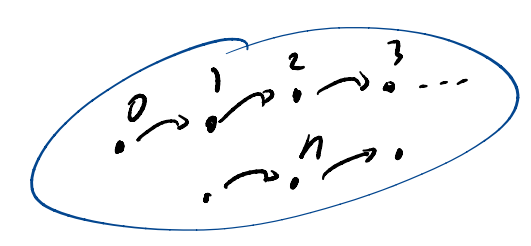
\includegraphics[width=0.5\textwidth]{Immagini/elementi_non_standard.png}
\end{figure}

Indaghiamo ora come funziona questa buffa nozione di $\leq$ per $\mathsf{Q}$, e vediamo che è proprio questa nozione di ordinamento che ci permette di distinguere tra elementi standard e non standard.

\begin{lemma}[Caratterizzazione di $a \leq \ol n$]
    $\forall n \in \NN$ vale che:
    \[ \mathsf Q \vdash \forall a (a \leq \ol n \leftrightarrow (a = \ol 0 \lor a = \ol 1 \lor \ldots \lor a = \ol n)) \]
    cioè ogni elemento del modello minore o uguale ad un numerale è uguale ad un numerale.
\end{lemma}

\begin{lemma}[Ogni elemento non standard è maggiore di ogni elemento standard]
    Sia $M \models \mathsf{Q}$, sia $\alpha \in M$ non standard, allora:
    \[ \forall n \in \NN \; M \models \alpha \leq \ol n \]
\end{lemma}

Dimostriamo in primis il secondo lemma, che è più semplice.

\begin{proof}
    Procediamo per induzione, metateorica, su $n$.
    \begin{itemize}
        \item[$\boxed{n = 0}$] Vogliamo dimostrare che $M \models \ol 0 \leq \alpha$, ovvero che $M \models \exists x \; x + \ol 0 = \alpha$, e questo, per la semantica di Tarski equivale a:
        \[ \exists x \in M \; x + 0 = \alpha \]
        prendendo $x = \alpha$, e poiché vale $\mathsf{Q}4$, otteniamo la tesi.
        \item[$\boxed{n \implies n+1}$] Vogliamo dimostrare che $M \models \alpha \leq \ol{n+1}$, come sopra, questo equivale a $M \models \exists x \; x + \ol{n+1} = \alpha$, e usando la semantica di Tarski diventa:
        \[ \exists x \in M \; x + \{\ldots\}_M \ol{n+1} = \alpha \]
        dove, essendo per definizione $\ol{n+1} = s(\ol n)$, vale che $\{\ldots\}_M \ol{n+1} = s(\{\ldots\}_M \ol n)$, e quindi, per $\mathsf{Q}4$, $x + \{\ldots\}_M \ol{n+1} = s(x + \{\ldots\}_M \ol n)$.
        Per $\mathsf{Q}7$ vale che $\alpha = s(\beta)$ - con $\beta$ non standard altrimenti si ha un assurdo, e banalmente, per $\mathsf{Q}2$, da $\ol{n+1} \leq \alpha$ segue che $\ol n \leq \beta$; usano infine l'ipotesi induttiva troviamo $y \in M$ tale che $y + \{\ldots\}_M \ol n = \beta$, e quindi $s(y + \{\ldots\}_M \ol n) = s(\beta)$,
        pertanto è sufficiente prendere $x = y$ per ottenere la tesi.
    \end{itemize}
\end{proof}

Vediamo infine la dimostrazione del primo lemma.

\begin{proof}
    Per induzione metateorica su $n$.
    \begin{itemize}
        \item[$\boxed{n = 0}$] Vogliamo dimostrare che $\mathsf{Q} \vdash \forall a (a \leq \ol 0 \leftrightarrow a = \ol 0)$, per definizione $a \leq 0$ equivale a $\exists x \; x + a = 0$, da cui segue subito $\leftarrow$, infatti in questo caso cerchiamo un $x$ tale che $x + 0 = 0$ e prendendo $x = 0$ otteniamo la tesi per $\mathsf{Q}3$.\\
        Per $\rightarrow$, se $a \leq 0$, allora $\exists x \; x + a = 0$  e vogliamo dimostrare che $a = 0$. Per assurdo, se $a \ne 0$, allora per $\mathsf{Q}7$ vale che $a = s(y)$ per qualche $y$, e quindi, per $\mathsf{Q}4$ vale che $x + s(y) = s(x + y) = 0$ che contraddice $\mathsf{Q}1$, assurdo.
        \item[$\boxed{n \implies n+1}$] Ci serve un lemma preliminare.
        \begin{lemma}[Il successore non fa salti]
            Nello stesso setting di prima vale:
            \[ \mathsf{Q} \vdash a \leq \ol{n+1} \leftrightarrow (a = 0) \lor \exists b (a = s(b) \land b \leq \ol n) \]
        \end{lemma}
        \begin{proof}
            In primis la tesi si può riscrivere come:
            \[ \mathsf{Q} \vdash \exists x (x + a = s(\ol n)) \leftrightarrow (a = 0) \lor \exists b (a = s(b) \land \exists y (y + b = \ol n)) \]
            Per $\leftarrow$, se $a = 0$, allora si prende come $x$ $\{\ldots\}_M s(\ol n)$ e si conclude per $\mathsf{Q}3$; se $a = s(b)$ e $y + b = \ol n$, allora per $\mathsf{Q}4$ vale che $y + s(b) = s(y + b) = s(\ol n)$, e quindi si prende $x = y$ per concludere.\\
            Viceversa, per $\rightarrow$, se $a \leq \ol{n+1}$, allora, se $a = 0$ abbiamo finito, altrimenti per $\mathsf{Q}7$ vale che $a = s(b)$ e dall'ipotesi $\exists x\; x + s(b) = s(\ol n)$, per $\mathsf{Q}4$ e $\mathsf{Q}2$ vale che $x + b = \ol n$, e quindi $b \leq \ol n$.
        \end{proof}
        Ora vogliamo dimostrare che:
        \[ \mathsf{Q} \vdash a \leq \ol{n+1} \leftrightarrow (a = \ol 0) \lor (a = \ol 1) \lor \ldots \lor (a = \ol{n+1}) \]
        Per $\leftarrow$, se $a = \ol{n+1}$ allora è banale che $a \leq \ol{n+1}$, se $a = \ol m$ con $m \leq n$, allora per ipotesi induttiva $\mathsf{Q} \vdash a \leq \ol n$, e quindi banalmente $a \leq \ol{n+1}$.\\
        Viceversa, per $\rightarrow$, se $a \leq \ol{n+1}$, allora per il lemma precedente vale che $a = 0$ o $a = s(b)$ con $b \leq \ol n$, se $a = 0$ allora abbiamo finito; altrimenti, se $a = s(b)$ con $b \leq \ol n$, allora per ipotesi induttiva $b = \ol m$ per qualche $m \leq n$,
        e quindi $a = s(\ol m) = \ol{m+1}$, con $m+1 \leq n+1$, e quindi abbiamo finito. 
    \end{itemize} 
\end{proof}

Finalmente possiamo dimostrare la prima parte della proposizione sull'equivalenza tra validità in $\NN$ e dimostrabilità in $\mathsf{Q}$ per le formule di classe $\Delta_0^0$ e $\Sigma_1^0$.
In particolare ora vediamo la dimostrazione di (1) e (2).

\begin{proof}
    Dimostriamo contemporaneamente (1) e (2).
    L'implicazione $\impliedby$ è banale poiché $\NN$ è un modello di $\mathsf{Q}$, per cui se $\mathsf{Q} \vdash \varphi$, allora $\NN \models \varphi$.\\
    Per dimostrare $\implies$, procediamo per induzione strutturale, contemporaneamente sia su (1) che su (2),sulla $L_\text{arit}$-formula $\varphi$ chiusa di classe $\Delta_0^0$, possiamo limitarci ai soli connettivi logici $\neg$ e $\land$, perché $\lor$ si ottiene da loro, e au quantificatori $\forall x \leq t$ e $\exists x \leq t$.
    \begin{itemize}
        \item \textcolor{MidnightBlue}{$\varphi$ è atomica} È il lemma già visto.
        \item \textcolor{MidnightBlue}{$\varphi = \neg \psi$} Abbiamo due casi o $\NN \models \neg \psi$ o $\NN \models \neg(\neg \psi)$, nel primo caso basta l'ipotesi induttiva (2): $\NN \models \neg \psi \implies \mathsf{Q} \vdash \neg \psi$.
        Il caso in cui invece $\NN \models \neg(\neg \psi)$ è banale, infatti sappiamo già che $\models \neg(\neg \psi) \iff \psi$ e che $\vdash \neg(\neg \psi) \iff \psi$, per cui si riduce all'ipotesi induttiva (1), cioè $\NN \models \psi \implies \mathsf{Q} \vdash \psi$.
        \item \textcolor{MidnightBlue}{$\varphi = \psi_1 \land \psi_2$} Come prima si danno due casi, quello in cui $\NN \models \psi_1 \land \psi_2$, che segue dalla semantica di Tarski:
        \begin{align*}
            \NN \models \psi_1 \land \psi_2 &\iff \NN \models \psi_1 \; \land \; \NN \models \psi_2 &&(\text{Tarski}) \\
                                              &\iff \mathsf{Q} \vdash \psi_1 \; \land \; \mathsf{Q} \vdash \psi_2 &&(\text{hp induttiva (1)}) \\
                                              &\iff \mathsf{Q} \vdash \psi_1 \land \psi_2 &&(\text{In$_{\land}$})
        \end{align*}
        Se invece $\NN \models \neg(\psi_1 \land \psi_2)$, allora (De Morgan) vale $\NN \models \neg\psi_1 \lor \neg\psi_2$; dunque si danno necessariamente due sottocasi.
        \begin{itemize}
            \item Se $\NN \models \neg\psi_1$, per ipotesi induttiva (2) abbiamo $\mathsf{Q} \vdash \neg\psi_1$, e quindi, usando In$_{\lor\cdot}$ e De Morgan, $\mathsf{Q} \vdash \neg(\psi_1 \land \psi_2)$.
            \item Se $\NN \models \neg\psi_2$, analogamente otteniamo $\mathsf{Q} \vdash \neg\psi_2$, e quindi $\mathsf{Q} \vdash \neg(\psi_1 \land \psi_2)$.
        \end{itemize}
        \item \textcolor{MidnightBlue}{$\varphi = \forall x \leq t \; \psi$} Assumiamo che $\NN \models \forall x \leq t \; \psi$, con $t$ termine chiuso perché lo è $\varphi$, e vogliamo dimostrare che $\mathsf{Q} \vdash \forall x \leq t \; \psi$.
        Sia $\{t\}_\NN = n$, per un lemma sappiamo che $\mathsf{Q} \vdash t = \ol n$, inoltre, per un altro lemma, $\mathsf{Q} \vdash \forall x \leq t \; \psi \leftrightarrow \forall x (x = \ol 0 \lor x = \ol 1 \lor \ldots \lor x = \ol n) \to \psi$,
        e questa formula equivale a:
        \[ (\forall x \; x = \ol 0 \to \psi) \land (\forall x \; x = \ol 1 \to \psi) \land \ldots \land (\forall x \; x = \ol n \to \psi) \]
        dove ciascuna delle sottoformule $\forall x \; x = \ol m \to \psi$ è proprio $\psi[m/x]$ - e questo si verifica tramite semantica di Tarski. Per cui la tesi si riduce a dimostrare che:
        \[ \mathsf{Q} \vdash \psi[0/x] \land \psi[1/x] \land \ldots \land \psi[n/x] \]
        ed a questo punto la tesi segue dal caso dell'$\land$.
        \item \textcolor{MidnightBlue}{$\varphi = \exists x \leq t \; \psi$} Esattamente come nel caso di sopra si arriva a voler dimostrare:
        \[ \mathsf{Q} \vdash \psi[0/x] \lor \psi[1/x] \lor \ldots \lor \psi[n/x] \]
        e anche in questo caso la tesi segue dal caso dell'$\lor$.
    \end{itemize}
\end{proof}

Infine vediamo anche la dimostrazione di (3).

\begin{proof}
    Vogliamo dimostrare che se $\varphi$ è chiusa di classe $\Sigma_1^0$, allora $\NN \models \varphi \iff \mathsf{Q} \vdash \varphi$. Come per il caso $\Delta_0^0$, l'implicazione $\impliedby$ è banale in quanto $\NN$ è un modello di $\mathsf{Q}$.\\
    Sia ora $\varphi = \exists x_1 \ldots \exists x_k \; \psi$, con $\psi$ di classe $\Delta_0^0$ e supponiamo che $\NN \models \varphi$, allora, per la semantica di Tarski + il lemma sulla sostituzione, esistono $n_1,\ldots,n_k \in \NN$ tali che:
    \[ \NN \models \psi[n_1/x_1,\ldots,n_k/x_k] \]
    ora, la formula ottenuta sostituendo i numerali $\ol{n_1},\ldots,\ol{n_k}$ a $x_1,\ldots,x_k$ è di classe $\Delta_0^0$, per cui vale l'ipotesi induttiva e si ha $\mathsf{Q} \vdash \psi[\ol{n_1}/x_1,\ldots,\ol{n_k}/x_k]$. Per concludere è sufficiente usare In$_{\exists}$ per $k$ volte e si ottiene $\mathsf{Q} \vdash \varphi$.
\end{proof}

A questo punto, dalle cose viste, sappiamo che il luogo di zero di una funzione ricorsiva è un insieme semidecidibile, e quindi è rappresentabile da una formula aritmetica di classe $\Sigma_1^0$,
e che per i parametri per cui la formula è vera, $\mathsf{Q}$ dimostra proprio la formula con i numerali al posto dei parametri, ovvero enunciato precisamente.

\begin{corollary}[Rappresentazione (del grafico) di funzioni ricorsive in $\mathsf{Q}$]
    Se $f : \NN^k \to \NN_\bot$ è ricorsiva, allora c'è $\varphi(x_1,\ldots,x_k,y)$ di classe $\Sigma_1^0$ tale che:
    \[ \forall x_1,\ldots,x_k\in\NN\;\forall y\in\NN\;(\mathsf{Q} \vdash \varphi(\ol{x_1},\ldots,\ol{x_k},\ol y) \iff f(x_1,\ldots,x_k)=y) \]
\end{corollary}

\begin{proof}
    La dimostrazione si ottiene considerando $\{f(x_1,\ldots,x_k) - y = 0\}$, che è semidecidibile, e per la caratterizzazione degli insiemi semidecidibili come gli insiemi di classe $\Sigma_1^0$,
    esiste una formula di classe $\Sigma_1^0$ tale $(x_1,\ldots,x_k,y) \in \{f(x_1,\ldots,x_k) - y = 0\}$ se e solo se $\NN \models \varphi(x_1,\ldots,x_k,y)$.
    Infine per la proposizione appena dimostrata vale che $\NN \models \varphi(x_1,\ldots,x_k,y)$ se e solo se $\mathsf{Q} \vdash \varphi(\ol{x_1},\ldots,\ol{x_k},\ol y)$, e questa è proprio l'equivalenza della tesi.
\end{proof}

Vediamo un risultato più forte, visto che il precedente è una condizione puntuale, nel senso che fissati a priori i parametri si ha l'equivalenza, possiamo migliorare l'equivalenza richiedendo che la funzione ricorsiva sia totale,
e ottenendo di conseguenza che la $\mathsf{Q}$ capisca che $f$ è una funzione, ovvero che per ogni $x_1,\ldots,x_k$ esiste un unico $y$ tale che $\varphi(x_1,\ldots,x_k,y)$ è vera, e che questo $y$ è proprio $f(x_1,\ldots,x_k)$.

\begin{lemma}[Rappresentazione di funzioni ricorsive totali in $\mathsf{Q}$]
    Sia $f : \NN^k \to \NN$ ricorsiva totale, allora c'è $\varphi(x_1,\ldots,x_k,y)$ di classe $\Sigma_1^0$ tale che:
    \[ \forall x_1,\ldots,x_k\in\NN\; \mathsf{Q} \vdash \forall y \; (\varphi(\ol{x_1},\ldots,\ol{x_k},y) \leftrightarrow y = \ol{f(x_1,\ldots,x_k)}) \]
\end{lemma}

\begin{proof}
    Sia $\psi$ una formula di classe $\Delta_0^0$ tale che per ogni $x_1, \dots, x_k, y \in \NN$:
    \[ y = f(x_1, \dots, x_k) \iff \mathsf{Q} \vdash \exists z_1 \dots \exists z_l \, \psi(\ol{x_1}, \dots, \ol{x_k}, \ol{y}, z_1, \dots, z_l) \]
    Consideriamo la formula $\varphi(x_1, \dots, x_k, y)$ definita come:
    \begin{align*}
        \exists N ( & \exists z_1 \le N \dots \exists z_l \le N \, (y \le N \land \psi(x_1, \dots, x_k, y, z_1, \dots, z_l)) \\
        \land & \forall t \le N \, \forall w_1 \le N \dots \forall w_l \le N \, (\psi(x_1, \dots, x_k, t, w_1, \dots, w_l) \to t = y) )
    \end{align*}
    Chiamiamo $\theta_1$ la prima riga tra parentesi e $\theta_2$ la seconda. Dimostriamo separatamente le due implicazioni:
    \begin{itemize}
        \item[$\boxed{\implies}$] Vogliamo mostrare che $\mathsf{Q} \vdash \forall y \, (\varphi(\ol{x_1}, \dots, \ol{x_k}, y) \to y = \ol{f(x_1, \dots, x_k)})$.
        Supponiamo, per assurdo, che non sia così e fissiamo $x_1, \dots, x_k$ e un modello $M \models \mathsf{Q}$ in cui esiste $y \ne f(x_1, \dots, x_k)$ tale che $M \models \varphi(\ol{x_1}, \dots, \ol{x_k}, y)$.
        Siccome $M \models \varphi$, possiamo fissare $N \in M$ tale che $N$ e $y$ soddisfino, in $M$, le formule $\theta_1$ e $\theta_2$. Si presentano due casi:
        \begin{itemize}
            \item \textit{Caso 1: $N$ è standard.} Per $\theta_1$, anche $y$ deve essere standard, ed esistono $z_1, \dots, z_l \in M$ standard tali che $M \models \psi(\ol{x_1}, \dots, \ol{x_k}, \ol{y}, \ol{z_1}, \dots, \ol{z_l})$. Siccome $\psi$ è $\Delta_0^0$, essa è decidibile, quindi $\mathsf{Q} \vdash \psi(\ol{x_1}, \dots, \ol{x_k}, \ol{y}, \ol{z_1}, \dots, \ol{z_l})$, il che implica $y = f(x_1, \dots, x_k)$, contro l'ipotesi.
            \item \textit{Caso 2: $N$ non è standard.} La formula $\theta_2$ asserisce che ogni testimone di $\psi$ minore di $N$ deve corrispondere a $y$. Per costruzione, esistono $z_1, \dots, z_l$ standard tali che $\mathsf{Q} \vdash \psi(\ol{x_1}, \dots, \ol{x_k}, \ol{f(x_1, \dots, x_k)}, \ol{z_1}, \dots, \ol{z_l})$. Poiché ogni numerale standard è minore di un elemento non standard $N$, ponendo $t = \ol{f(x_1, \dots, x_k)}$, i testimoni standard soddisfano la premessa di $\theta_2$, da cui $M \models \ol{f(x_1, \dots, x_k)} = y$, assurdo.
        \end{itemize}
        \item[$\boxed{\impliedby}$] Vogliamo mostrare che $\mathsf{Q} \vdash \forall y \, (y = \ol{f(x_1, \dots, x_k)} \to \varphi(\ol{x_1}, \dots, \ol{x_k}, y))$.
        È sufficiente provare che $\mathsf{Q} \vdash \varphi(\ol{x_1}, \dots, \ol{x_k}, \ol{f(x_1, \dots, x_k)})$.\\
        Siano $z_1, \dots, z_l$ tali che $\mathsf{Q} \vdash \psi(\ol{x_1}, \dots, \ol{x_k}, \ol{f(x_1, \dots, x_k)}, \ol{z_1}, \dots, \ol{z_l})$.
        Scegliamo $N := \max\{f(x_1, \dots, x_k), z_1, \dots, z_l\}$, in ogni modello $M \models \mathsf{Q}$, il numerale $\ol{N}$ funge da limitazione corretta:
        \begin{enumerate}
            \item $\theta_1$ è soddisfatta in $M$ dai testimoni $\ol{z_1}, \dots, \ol{z_l}$ e $\ol{f(x_1, \dots, x_k)}$, che sono tutti minori o uguali a $\ol{N}$.
            \item Per $\theta_2$, se $M \models t \le \ol{N} \land \psi(\dots, t, \dots)$, allora $t$ deve essere standard (perché minore di un numerale standard). Per la costruzione di $\psi$, l'unico valore standard che soddisfa la relazione è proprio $f(x_1, \dots, x_k)$, quindi $M \models t = \ol{f(x_1, \dots, x_k)}$.
        \end{enumerate}
    \end{itemize}
\end{proof}

\section{Teoremi di incompletezza}
\subsection{Numerazione di Gödel}

Una numerazione di Gödel è in generale un modo di associare ad ogni formula di un linguaggio una numero naturale, il modo specifico di farlo non è importante, l'importante è che sia una codifica efficace, ovvero che sia possibile risalire alla formula a partire dal numero e viceversa,
e che sia possibile decidere se un numero è la codifica di una formula o meno.

Fissiamo una codifica effettiva dei simboli di $L_{\text{arit}}$ mediante numeri naturali distinti e usiamo la codifica di liste
$\langle a_1,\ldots,a_n\rangle$ introdotta prima per concatenare i codici. Usiamo i tag per numerare i simboli, usiamo il sistema ridotto, quindi i simboli numerati sono:
\[ \begin{array}{cccccccccc}
    & \textcolor{purple}{\bot} & \textcolor{purple}{\to} & \textcolor{purple}{\forall} & \textcolor{purple}{=} & \textcolor{purple}{0} & \textcolor{purple}{s} & \textcolor{purple}{+} & \textcolor{purple}{\cdot} & \textcolor{purple}{x_i} \\
    & 0 & 1 & 2 & 3 & 4 & 5 & 6 & 7 & 8+i \\
    & \textcolor{green!50!black}{\#\bot} & \textcolor{green!50!black}{\#\to} & \textcolor{green!50!black}{\#\forall} & \textcolor{green!50!black}{\#=} & \textcolor{green!50!black}{\#0} & \textcolor{green!50!black}{\#s} & \textcolor{green!50!black}{\#+} & \textcolor{green!50!black}{\#\cdot} & \textcolor{green!50!black}{\#x_i}
\end{array}\]
quindi d'ora in poi $\#\cdot$ è il numero che abbiamo scelto per codificare il simbolo di moltiplicazione, $\#\forall$ è il numero che abbiamo scelto per codificare il quantificatore universale, e così via.
La scelta concreta dei numeri è irrilevante: ciò che conta è che le operazioni sintattiche fondamentali siano funzioni ricorsive.

\begin{definition}[Codifica di termini e formule]
    Fissata una numerazione dei simboli di $L_{\text{arit}}$, possiamo definire ricorsivamente la \vocab{codifica di Gödel} (o \vocab{numerazione di Gödel}) $\ulcorner\cdot\urcorner$ come segue.
    \begin{itemize}
        \item $L_{\text{arit}}$-termini:
        \[ \ulcorner 0\urcorner := \langle\#0\rangle \qquad \ulcorner x_i\urcorner := \langle\#x_i\rangle \]
        \[ \ulcorner s(t)\urcorner := \langle\#s,\ulcorner t\urcorner\rangle\qquad \ulcorner t_1+t_2\urcorner := \langle\#+,\ulcorner t_1\urcorner,\ulcorner t_2\urcorner\rangle \]
        \[ \ulcorner t_1\cdot t_2\urcorner := \langle\#\cdot,\ulcorner t_1\urcorner,\ulcorner t_2\urcorner\rangle \]
        \item $L_{\text{arit}}$-formule:
        \[ \ulcorner t_1=t_2\urcorner := \langle\#=,\ulcorner t_1\urcorner,\ulcorner t_2\urcorner\rangle\qquad \ulcorner\neg\varphi\urcorner := \langle\#\neg,\ulcorner\varphi\urcorner\rangle \]
        \[ \ulcorner\varphi\to\psi\urcorner := \langle\#\to,\ulcorner\varphi\urcorner,\ulcorner\psi\urcorner\rangle\qquad \ulcorner\forall x_i\,\varphi\urcorner := \langle\#\forall,\#x_i,\ulcorner\varphi\urcorner\rangle \]
    \end{itemize}
\end{definition}

Abbiamo così ottenuto una numerazione iniettiva di ogni $L_{\text{arit}}$-termine e di ogni $L_{\text{arit}}$-formula.
Il nostro obiettivo sarà dimostrare il seguente lemma.

\begin{lemma}[Lemma di diagonalizzazione di Gödel]
    Sia $\varphi$ una formula aritmetica, esiste una formula aritmetica $\textcolor{purple}{\psi}$ tale che:
    \[ \mathsf{Q} \vdash \textcolor{purple}{\psi} \leftrightarrow \varphi[\overline{\ulcorner\textcolor{purple}{\psi}\urcorner}/x_1] \]
    cioè per ogni formula con una variabile libere né esiste un'altra che è vera se e solo se è vera ``$\varphi(\psi)$".
\end{lemma}

Di fatto il lemma ci dà una specie di teorema di punto fisso per le formule, cioè per ogni formula ne esiste un'altra 
la cui validità è equivalente alla validità della proprietà che la prima formula esprime valida per la seconda. In altre parole, c'è sempre una formula che dice di sé stessa che è vera se e solo se è vera una certa proprietà per lei.
La proprietà che ci interesserà sarà ``io sono dimostrabile''.\\
Osserviamo che non tutti i numeri naturali sono codici di formule, per la nostra codifica, da cui la necessità di poter decidere se un numero è codice di una formula o meno.

\begin{remark}[$n$ è il codice di una formula]
    Il predicato $\textsf{For}(n) :=$ ``$n$ è codice di una formula'' è PR.
\end{remark}

\begin{proof}
    Per decidere se $n$ è codice di una formula, basta verificare che il primo simbolo della lista sia un connettivo o che la formula sia atomica, per cui il
    predicato $\textsf{For}(n)$ si può definire per casi come segue:
    \begin{align*}
        \textsf{For}(n) &= (\nth(n,0) = \#\bot \land \length(n) = 1) \\
                        &\land (\nth(n,0) = \#= \land \length(n) = 3 \land \textsf{Term}(\nth(n,1)) \land \textsf{Term}(\nth(n,2))) \\
                        &\land (\nth(n,0) = \#\neg \land \length(n) = 2 \land \textsf{For}(\nth(n,1))) \\
                        &\land (\nth(n,0) = \#\to \land \length(n) = 3 \land \textsf{For}(\nth(n,1)) \land \textsf{For}(\nth(n,2))) \\
                        &\land (\nth(n,0) = \#\forall \land \length(n) = 3 \land \nth(n,1) \geq 8 \land \textsf{For}(\nth(n,2)))
    \end{align*}
    dove aggiungiamo gli altri $\textsf{For}$ ricorsivamente, per la precisione per ricorsione sul corso dei valori, perché la formula codificata da $n$ è una formula se e solo se le sottoformule codificate dai sotto-codici sono formule,
    ovviamente, essendo la definizione fatta da un'intersezione finita di predicati PR, $\textsf{For}$ è PR. Osserviamo infine che c'è necessità anche di introdurre il predicato $\textsf{Term}$, che dice se un numero è codice di un termine, ma anche questo è PR, e si definisce in modo seguente:
    \begin{align*}
        \textsf{Term}(n) &= (\nth(n,0) = \#0 \land \length(n) = 1) \\
                        &\land (\nth(n,0) = \#x_i \land \length(n) = 1) \\
                        &\land (\nth(n,0) = \#f_i \land \length(n) = 1) \\
                        &\land (\nth(n,0) = \#s \land \length(n) = 2 \land \textsf{Term}(\nth(n,1))) \\
                        &\land (\nth(n,0) = \#+ \land \length(n) = 3 \land \textsf{Term}(\nth(n,1)) \land \textsf{Term}(\nth(n,2))) \\
                        &\land (\nth(n,0) = \#\cdot \land \length(n) = 3 \land \textsf{Term}(\nth(n,1)) \land \textsf{Term}(\nth(n,2)))
    \end{align*}
    anche in questo caso la definizione è fatta per ricorsione sul corso dei valori intersecando cose PR.
\end{proof}

\pagebreak
\begin{remark}[$n$ è il codice di un numerale]
    Definiamo la funzione $\textsf{Num}(n) : n \mapsto \ulcorner\ol n\urcorner$, ovvero la funzione che associa ad ogni numero naturale il numerale corrispondente,
    tale funzione è PR.
\end{remark}

\begin{proof}
    Come prima si può definire a partire da altre funzioni PR come segue:
    \[ \textsf{Num}(n) := \begin{cases}
        \textsf{Num}(0) = \ulcorner 0\urcorner = \langle\#0\rangle \\
        \textsf{Num}(n+1) = \ulcorner s(\ol n)\urcorner = \langle\#s, \textsf{Num}(n)\rangle
    \end{cases} \]
\end{proof}


\begin{remark}[Codice della sosituzione]
    Sia $\textsf{Sub}(\ulcorner\varphi\urcorner, i, \ulcorner t\urcorner) := \ulcorner\varphi[t/x_i]\urcorner$ la funzione che associa il codice di una formula,
    di una variabile e di un termine al codice ottenuto facendo la sostituzione del termine al posto della variabile, tale funzione è PR.
\end{remark}

\begin{proof}
    Anche questa può essere definita a partire da funzioni PR:
    \[ \textsf{Sub}(n,i,x) := \begin{cases}
        0 & \text{se $\neg\textsf{For}(n)$} \\
        \langle \#\bot \rangle & \text{se $n = \langle\#\bot\rangle$} \\
        \langle \#=, \textsf{Sub}(a,i,x), \textsf{Sub}(b,i,x) \rangle & \text{se $n = \langle\#=,\ulcorner a\urcorner,\ulcorner b\urcorner\rangle$} \\
        \langle \#\neg, \textsf{Sub}(a,i,x) \rangle & \text{se $n = \langle\#\neg,\ulcorner a\urcorner\rangle$} \\
        \langle \#\to, \textsf{Sub}(a,i,x), \textsf{Sub}(b,i,x) \rangle & \text{se $n = \langle\#\to,\ulcorner a\urcorner,\ulcorner b\urcorner\rangle$} \\
        \langle \#\forall, j, \textsf{Sub}(a,i,x) \rangle & \text{se $n = \langle\#\forall,j,\ulcorner a\urcorner\rangle$ e $j \ne i$} \\
        \langle \#\forall, j, a \rangle & \text{se $n = \langle\#\forall,j,\ulcorner a\urcorner\rangle$ e $j = i$}
    \end{cases} \]
\end{proof}

Possiamo quindi dimostrare il lemma di diagonalizzazione di Gödel.

\begin{proof}
    \textcolor{MidnightBlue}{Come nel caso di teorema di punto fisso per le funzioni ricorsive, vediamo informalmente cosa vorremmo fare, e poi lo formalizziamo. 
    Supponiamo che tutto sia applicabile a tutto allora considero la funzione $f(x) := x(x)$, ovvero la funzione che prende una 
    formula e la applica a se stessa, il nostro scopo è trovare $\psi = \varphi(\psi)$ - dove con l'$=$ intendiamo l'equivalenza, allora se potessimo definire $f$ potremmo definire
    la formula $\theta := \varphi(f(x))$ e quindi applicando $\theta$ a se stessa otteniamo $\theta(\theta) = \varphi(f(\theta)) = \varphi(\theta(\theta))$ e chiamando $\theta(\theta) := \psi$ avremmo finito.}\\
    La vera funzione $f$ che vogliamo definire fa praticamente la stessa cosa, ma usa i codici invece che le formule:
    \[ f : \NN \to \NN : \ulcorner \alpha\urcorner \mapsto \ulcorner \alpha[\overline{\ulcorner\alpha\urcorner}/x_k]\urcorner \quad \text{con $x_k \in \vl(\alpha)$} \]
    tale funzione è PR, perché si può definire come:
    \[ f(n) = \textsf{Sub}(n,k,\textsf{Num}(n)) \]
    dove la cosa sostituita è appunto il numerale corrispondente al numero di Gödel della formula. Ora vorremmo definire la nostra ``$\theta := \varphi(f(x))$'',
    tecnicamente, in primis applichiamo il lemma di rappresentazione di funzioni ricorsive in $\mathsf{Q}$ alla funzione ricorsiva totale $f$, per quel lemma esiste una formula $\pi$,
    per la quale possiamo assumere (WLOG a meno di rinominare) che $\vl(\pi) \subseteq \{x_1,\ldots,x_k\}$, con $k > 1$,e vale:
    \[ \forall n \in \mathbb N \; \mathsf{Q} \vdash \forall x_1 (\pi[\overline{n}/x_k] \leftrightarrow x_1 = \overline{f(n)}) \]
    dove $\pi[\overline{n}/x_k]$ è in vece della usuale $\pi(\ol n,x_1)$ del lemma, e scelgo proprio $x_k$ perché è quella della definizione di $f$.
    Ora definiamo $\theta := \forall x_1 \pi \to \varphi$ e $\psi := \theta[\ol{\ulcorner\theta\urcorner}/x_k]$ e verifichiamo la tesi.
    Per la costruzione di $\pi$, usando $\ulcorner\theta\urcorner \in \NN$ abbiamo:
    \[ \mathsf{Q} \vdash \forall x_1 (\pi[\overline{\ulcorner\theta\urcorner}/x_k] \leftrightarrow x_1 = \overline{f(\ulcorner\theta\urcorner)}) \]
    e per la definizione di $f(\ulcorner\theta\urcorner) = \ulcorner\theta[\overline{\ulcorner\theta\urcorner}/x_k]\urcorner$, che unita alla definizione di $\psi$ è
    $f(\ulcorner\theta\urcorner) = \ulcorner\psi\urcorner$, dà:
    \[ \mathsf{Q} \vdash \forall x_1 (\pi[\overline{\ulcorner\theta\urcorner}/x_k] \leftrightarrow x_1 = \overline{\ulcorner\psi\urcorner}) \]
    Ora la formula $\psi = \theta[\ol{\ulcorner\theta\urcorner}/x_k] = (\forall x_1 \pi \to \varphi)[\ol{\ulcorner\theta\urcorner}/x_k]$, sfruttando il fatto che $x_k$ non compare in $\varphi$, per ipotesi la sua variabile libera è $x_1$, è equivalente a:
    \[ \psi \equiv \forall x_1 \pi[\ulcorner\theta\urcorner/x_k] \to \varphi \]
    e quindi, usando la formula precedente, posso rimpiazzare $\pi[\ulcorner\theta\urcorner/x_k]$ con $x_1 = \overline{\ulcorner\psi\urcorner}$, ottenendo:
    \[ \mathsf{Q} \vdash \psi \leftrightarrow \forall x_1 (x_1 = \overline{\ulcorner\psi\urcorner} \to \varphi) \]
    infine, osservo che $\forall x_1 (x_1 = \overline{\ulcorner\psi\urcorner} \to \varphi)$ è equivalente a $\varphi[\overline{\ulcorner\psi\urcorner}/x_1]$.
    Per $\to$:
    \[
    \text{El}_{\to}\frac
    {\text{El}_{\forall}\frac{\text{Ax}\frac{}{\forall x_1 (x_1 = \overline{\ulcorner\psi\urcorner} \to \varphi) \vdash \forall x_1 (x_1 = \overline{\ulcorner\psi\urcorner} \to \varphi)}}{\forall x_1 (x_1 = \overline{\ulcorner\psi\urcorner} \to \varphi) \vdash \overline{\ulcorner\psi\urcorner} = \overline{\ulcorner\psi\urcorner} \to \varphi[\overline{\ulcorner\psi\urcorner}/x_1]}
    \qquad
    \text{Wk}\frac{\text{In}_{=}\frac{}{\vdash \overline{\ulcorner\psi\urcorner} = \overline{\ulcorner\psi\urcorner}}}{\forall x_1 (x_1 = \overline{\ulcorner\psi\urcorner} \to \varphi) \vdash \overline{\ulcorner\psi\urcorner} = \overline{\ulcorner\psi\urcorner}}}
    {\forall x_1 (x_1 = \overline{\ulcorner\psi\urcorner} \to \varphi) \vdash \varphi[\overline{\ulcorner\psi\urcorner}/x_1]}
    \]
    Per il viceversa:
    \[
    \text{In}_{\forall}\frac
    {\text{In}_{\to}\frac
    {\text{El}_{=}\frac
    {\text{El}_{=}\frac
    {\text{Ax}\frac{}{x_1 = \overline{\ulcorner\psi\urcorner} \vdash x_1 = \overline{\ulcorner\psi\urcorner}}
    \qquad
    \text{Wk}\frac{\text{In}_{=}\frac{}{\vdash x_1 = x_1}}{x_1 = \overline{\ulcorner\psi\urcorner} \vdash x_1 = x_1}}
    {x_1 = \overline{\ulcorner\psi\urcorner} \vdash \overline{\ulcorner\psi\urcorner} = x_1}
    \qquad
    \text{Wk}\frac{\text{Ax}\frac{}{\varphi[\overline{\ulcorner\psi\urcorner}/x_1] \vdash \varphi[\overline{\ulcorner\psi\urcorner}/x_1]}}{x_1 = \overline{\ulcorner\psi\urcorner},\varphi[\overline{\ulcorner\psi\urcorner}/x_1] \vdash \varphi[\overline{\ulcorner\psi\urcorner}/x_1]}}
    {x_1 = \overline{\ulcorner\psi\urcorner},\varphi[\overline{\ulcorner\psi\urcorner}/x_1] \vdash \varphi}
    }{\varphi[\overline{\ulcorner\psi\urcorner}/x_1] \vdash x_1 = \overline{\ulcorner\psi\urcorner} \to \varphi}
    }{\varphi[\overline{\ulcorner\psi\urcorner}/x_1] \vdash \forall x_1 (x_1 = \overline{\ulcorner\psi\urcorner} \to \varphi)}
    \]
    dove nell'ultimo passaggio ho usato In$_\forall$, e posso farlo perché $x_1 \notin \vl(\varphi[\overline{\ulcorner\psi\urcorner}/x_1])$.
    Quindi:
    \[ \mathsf{Q} \vdash \psi \leftrightarrow \varphi[\overline{\ulcorner\psi\urcorner}/x_1] \]
    che è la tesi.
\end{proof}

\subsection{Predicato di dimostrazione}
Il nostro scopo in questa sezione sarà dimostrare che esiste una $L_{\text{arit}}$-formula che dice di sé stessa che è dimostrabile, per poi combinarla col lemma di diagonalizzazione di Gödel
ed ottenere il primo teorema di incompletezza di Gödel. Richiamiamo una definizione già data, ma senza formalizzare bene le enumerazioni di Gödel.

\begin{definition}[Teoria ricorsivamente (o semidecidibilmente) assiomatizzabile]
    Una teoria $T$ è \vocab{ricorsivamente assiomatizzabile}, o \vocab{semidecidibilmente assiomatizzabile}, se:
    \[ T = \{\sigma : P(\ulcorner\sigma\urcorner) \ne \bot \} \]
    con $P$ una funzione ricorsiva parziale, ovvero esiste un algoritmo che stabilisce se una formula è un assioma di $T$ o no.
\end{definition}

In realtà, per via di un trucco, possiamo sempre supporre che l'insieme di assiomi sia addirittura decidibile.

\begin{exercise}[Teorema di Craig]
    Sia $T := \{\varphi : P(\ulcorner\varphi\urcorner) = 0 \}$ ricorsivamente assiomatizzabile, allora esiste una teoria \vocab{decidibilmente assiomatizzabile}, i.e. l'insieme dei codici degli assiomi è decidibile, tale che $T$ e $T'$ sono equivalenti.
\end{exercise}

\begin{soln}
    Per ipotesi, $T$ è descrivibile come insieme semidecidibile, quindi esiste una funzione ricorsiva totale $f$ tale che $T = \{ \varphi : \exists n \, f(n) = \ulcorner\varphi\urcorner \}$,
    quindi possiamo supporre $T = \{\varphi_1, \varphi_2, \ldots\}$, WLOG $f(1) = \ulcorner\varphi_1\urcorner$, $f(2) = \ulcorner\varphi_2\urcorner$ e così via.\\
    Ora, definiamo la nuova lista di assiomi di $T'$ come segue:
    \begin{align*}
        \varphi_1' &:= \varphi_1 \\
        \varphi_2' &:= \varphi_2 \land \varphi_2 \\
        \varphi_3' &:= \varphi_3 \land \varphi_3 \land \varphi_3 \\
        &\vdots
    \end{align*}
    si verifica banalmente, al livello sintattico, che $T$ è equivalente a $T'$.
    Inoltre, se poniamo $h(n) := \ulcorner\varphi_n'\urcorner$, la funzione $h : \NN \to \NN$ è ricorsiva totale (si ottiene da $f$ componendo con operazioni sintattiche ricorsive, cioè codifica e congiunzione iterata).
    Quindi posso definire il test totale ricorsivo degli assiomi di $T'$ come:
    \[ g(z) := \begin{cases}
        0 & \text{se $\exists n \le z\; h(n) = z$} \\
        1 & \text{altrimenti}
    \end{cases} \]
    infatti $g(z)=0$ se e solo se $z$ è codice di un assioma di $T'$ - la ricerca è limitata ai primi $z$ numeri perché altrimenti potrebbe non fermarsi e venire $\bot$\footnote{Andrebbe controllato inoltre che il predicato per la definizione per casi sia ricorsivo totale.}; inoltre $g$ è ricorsiva totale, in quanto è definita per casi su una funzione ricorsiva totale.
\end{soln}

\begin{lemma}[Predicato di dimostrazione]
    Sia $T$ una teoria aritmetica ricorsivamente assiomatizzabile, allora esiste un predicato PR $\mathsf{Dim}_T(x,y)$ tale che:
    \[ T \vdash \varphi \iff \NN \models \exists d\,\mathsf{Dim}_T(d,\ulcorner\varphi\urcorner) \]
    ovvero $T$ dimostra $\varphi$ se e solo se esiste un codice $d$ di una dimostrazione di $\varphi$ in $T$.
\end{lemma}

\begin{proof}
    In primis diciamo come è codificata una dimostrazione, sappiamo che $T \vdash \varphi$ se esiste una sequenza finita di formule - anche se tecnicamente per noi è sempre una sequenza finita di sequenti\footnote{Per essere precisi la codifica vera nel nostro sistema $\textsf{ND}$ è la codifica di un sequente $\sigma_i = \ulcorner \varphi_1, \varphi_2, \ldots, \varphi_n \vdash \psi \urcorner$,
    che possiamo codificare come $\langle \langle \ulcorner \varphi_1\urcorner, \ulcorner\varphi_2\urcorner, \ldots, \ulcorner\varphi_n\urcorner\rangle, \ulcorner\psi\urcorner\rangle$, codificato un sequente in questo modo, codifichiamo la dimostrazione come lista di sequenti $\ulcorner \sigma_1, \sigma_2, \ldots, \sigma_m\urcorner$ come $\langle \ulcorner\sigma_1\urcorner, \ulcorner\sigma_2\urcorner, \ldots, \ulcorner\sigma_m\urcorner\rangle$ così abbiamo codificato esattamente la nostra definizione di dimostrazione.} -
    con l'ultima che è $\varphi$ e quelle precedenti che sono o assiomi o si ottengono da quelle prima usando le regole di inferenza del sistema di deduzione naturale $\textsf{ND}$, quindi una dimostrazione $\delta$ la si può codificare come la lista delle formule che la compongono:
    \[ \ulcorner \delta\urcorner := \langle \ulcorner\delta_1\urcorner, \ulcorner\delta_2\urcorner, \ldots, \ulcorner\delta_n\urcorner \rangle \]
    dove $\delta_n$ è la formula finale, ovvero $\varphi$.\\
    Ora possiamo definire $\mathsf{Dim}_T(d,x)$ traducendo il significato della definizione di dimostrazione in una definizione PR:
    \begin{align*}
        \textsf{Dim}_T(d,x) &:= \nth(d,\length(d) \dotminus 1) = x \\
                            &\land \forall i < \length(d) \; \text{``$\nth(d,i)$ è o un assioma di $T$ o segue da quelli prima...''}
    \end{align*}
    ora ``$\nth(d,i)$ è un assioma'' è esprimibile come predicato PR, perché per ipotesi $T$ è ricorsivamente assiomatizzabile, quindi esiste una funzione ricorsiva totale da mettere in quel posto;
    per ``$\nth(d,i)$ segue dalle formule prima usando le regole di inferenza'' basta scrivere un lungo OR che esprima tutti le possibili applicazioni delle regole di inferenza, ad esempio:
    \[ \text{In}_{\to} \frac{T \vdash \varphi \quad T \vdash \varphi \to \psi}{T \vdash \psi} \]
    equivale a:
    \[ \exists j < i \; \exists t < i \; \nth(d,t) = \textsf{implica}(\nth(d,j), \nth(d,i)) \]
    dove $\textsf{implica}$ è la funzione PR che prende i codici di due formule e restituisce il codice della formula che è l'implicazione tra le due - cioè $\langle \#\to, \nth(d,j), \nth(d,i)\rangle$ - e tutti i casi 
    si fanno così (l'unico caso più complicato è quello di In$_\forall$ dove bisogna controllare che la variabile libera sia effettivamente libera nelle premesse e quindi introdurre $\textsf{free}(y,i) := ``\text{$x_i$ è libera in $y$}''$).
    Abbiamo quindi definito $\textsf{Dim}_T(d,x)$ come predicato PR via ricorsione e casi.
\end{proof}

\subsection{Primo teorema di incompletezza}

\begin{theorem}[Primo teorema di incompletezza di Gödel]
    Sia $T$ una teoria aritmetica tale che:
    \begin{enumerate}[(i)]
        \item $T$ è ricorsivamente assiomatizzabile;
        \item $T \vdash \mathsf{Q}$ e $\NN \models T$;
    \end{enumerate}
    allora $T$ è incompleta.
\end{theorem}

\begin{proof}
    Lo scopo è costruire una formula $\gamma$ che dica ``io non sono dimostrabile in $T$'', ovvero una formula che per $T$ è proprio equivalente al fatto che non esiste una dimostrazione per lei:
    \[ T \vdash \gamma \leftrightarrow \neg\exists d\,\mathsf{Dim}_T(d,\ulcorner\gamma\urcorner) \]
    Per costruire $\gamma$ basta applicare il lemma di diagonalizzazione alla formula $\varphi(x) := \neg\exists d\,\mathsf{Dim}_T(d,x)$, e otteniamo $\gamma$, che per il lemma di diagonalizzazione
    soddisfa esattamente la condizione di cui sopra. Vediamo ora che $T$ non dimostra né $\gamma$ né $\neg\gamma$.
    \begin{itemize}
        \item Supponiamo $T \vdash \gamma$, allora esiste il codice di una dimostrazione di $\gamma$ in $T$, chiamiamolo $\delta$,
        quindi $\textsf{Dim}_T(\ulcorner\delta\urcorner, \ulcorner\gamma\urcorner)$ è un predicato PR vero, che per il lemma di rappresentazione di funzioni ricorsive totali in $\mathsf{Q}$,
        significa che $\mathsf{Q} \vdash \textsf{Dim}_T(\ulcorner\delta\urcorner, \ulcorner\gamma\urcorner)$, e quindi $T \vdash \textsf{Dim}_T(\ulcorner\delta\urcorner, \ulcorner\gamma\urcorner)$ e per In$_\exists$ si ha $T \vdash \exists d\,\mathsf{Dim}_T(d,\ulcorner\gamma\urcorner)$;
        ma $T$ dimostra anche $\gamma$, che per $T$ equivale a $\neg\exists d\,\mathsf{Dim}_T(d,\ulcorner\gamma\urcorner)$, quindi $T$ dimostra sia $\textsf{Dim}_T(\ulcorner\delta\urcorner, \ulcorner\gamma\urcorner)$ che $\neg\exists d\,\mathsf{Dim}_T(d,\ulcorner\gamma\urcorner)$ $\lightning$, perché $T$ è coerente per ipotesi (ii).
        \item Supponiamo $T \vdash \neg\gamma$, allora, doppia negazione, $T$ dimostra $\exists d\,\mathsf{Dim}_T(d,\ulcorner\gamma\urcorner)$, ma allora per (ii) $\NN \models \exists d\,\mathsf{Dim}_T(d,\ulcorner\gamma\urcorner)$,
        che per la semantica di Tarski equivale a dire che $\exists d \in \NN \; \NN \models \mathsf{Dim}_T(\ol d, \ulcorner\gamma\urcorner)$; segue che $d$ codifica una dimostrazione di $\gamma$ in $T$, per cui $T \vdash \gamma$, assurdo.
    \end{itemize} 
\end{proof}

Ora questo teorema è un po' più forte del necessario e si possono indebolire le ipotesi per ottenere il teorema di Rosser.

\begin{theorem}[Teorema di Rosser]
    Sia $T$ una teoria aritmetica tale che:
    \begin{enumerate}[(i)]
        \item $T$ è ricorsivamente assiomatizzabile;
        \item $T \vdash \mathsf{Q}$;
        \item $T$ è coerente;
    \end{enumerate}
    allora $T$ è incompleta.
\end{theorem}

Nella dimostrazione del primo teorema di incompletezza di Gödel abbiamo fatto uso del fatto che $\NN$ fosse modello di $T$, oltre alla coerenza di $T$, quindi quella dimostrazione non può essere riciclata.

\begin{proof}[Dimostrazione \textup{(IDEA)}]
    L'idea della dimostrazione, che non vediamo, è quella di usare una formula che dice ``se ci fosse una mia dimostrazione, allora ci sarebbe anche una dimostrazione di una mia negazione più corta'', ovvero:
    \[ \mathsf{Q} \vdash\varphi \leftrightarrow \forall d \, \textsf{Dim}_T(d,\ulcorner\varphi\urcorner) \to \exists d' \leq d \, \textsf{Dim}_T(d',\ulcorner\neg\varphi\urcorner) \]
    e questo è un modo per ottenere comunque una formula che dice di sé stessa che è non dimostrabile - basta pensare alla negazione.
\end{proof}

\begin{definition}[Teoria decidibile]
    Una teoria $T$ è \vocab{decidibile} se l'insieme dei codici delle formule dimostrate da $T$ è decidibile, ovvero esiste una funzione ricorsiva totale $P$ tale che:
    \[ \{\ulcorner\sigma\urcorner : T \vdash \sigma\} = \{ i \in \NN : P(i) = 0 \} \]
    analogamente si può definire una teoria \vocab{semidecidibile}.
\end{definition}

\begin{proposition}[Completamento decidibile]
    Sia $T$ una teoria coerente e decidibile, allora esiste un'estensione coerente $T'$ di $T$ che è completa e decidibile.
\end{proposition}

\begin{proof}
    Per ipotesi possiamo fissare un'enumerazione delle formule chiuse $\{\varphi_i\}_{i\in\NN}$ e definiamo per ricorsione:
    \[ T_0:=T \]
    \[ T_{i+1}:=\begin{cases}
        T_i\cup\{\varphi_i\} & \text{se $T_i\nvdash\neg\varphi_i$}\\
        T_i & \text{altrimenti}
    \end{cases} \]
    cioè in ogni step se la $i$-esima teoria non dimostra la negazione dell'$i$-esima formula, allora la aggiungo, altrimenti lascio tutto com'è.\\
    Ora, ponendo $T' := \bigcup_{i\in\NN} T_i$, si verifica che $T'$ è un'estensione di $T$ coerente, infatti se $T'$ fosse incoerente, allora $T' \vdash \bot$,
    quindi per compattezza esisterebbe un sottoinsieme finito $T'' \subseteq T'$ tale che $T'' \vdash \bot$, per cui esiste un $i_0$ tale che $T'' \subseteq T_{i_0}$, ma allora $T_{i_0} \vdash \bot$,
    che è assurdo perché si verifica per induzione che ogni $T_i$ è coerente.\\
    $T'$ è decidibile, presa $\{\sigma_j\}_{j \in \NN}$ un'enumerazione di tutte le $L_{\text{arit}}$-formule, e fissato un algoritmo che decide se una formula è dimostrata da $T$ o no,
    basta testare, per $\sigma = \sigma_k$, per qualche $k > 0$, se $T_k \vdash \neg\sigma$ o no, e questo posso farlo perché $T_k = T \cup \{\varphi_0, \ldots, \varphi_{k-1}\}$ e:
    \[ T_k \vdash \neg\sigma \iff T \vdash (\varphi_0 \land \ldots \land \varphi_{k-1}) \to \neg\sigma\]
    e questo è decidibile per ipotesi, se il risultato dell'algoritmo è falso, allora $T_{k+1} = T_k \cup \{\sigma\}$ e $T' \vdash \sigma$, altrimenti $T_{k+1} = T_k$ e $T' \vdash \neg\sigma$. Nel caso $k = 0$ la tesi è banale perché $T_0 = T$ è decidibile per ipotesi.\\
    Infine, $T'$ è completa, fissata una enumerazione $\{\varphi_i\}_{i\in\NN}$ di tutte le $L_{\text{arit}}$-formule, allora, per ogni $\varphi_i$, si ha che 
    o $T_i \nvdash \neg\varphi_i$, e allora $T_{i+1} \vdash \varphi_i$, oppure $T_i \vdash \neg\varphi_i$, nel primo caso ottengo $T' \vdash \varphi_i$, nel secondo caso $T' \vdash \neg\varphi_i$, quindi $T'$ è completa.
\end{proof}

\begin{corollary}[$\mathsf Q$ e $\mathsf{PA}$ non sono decidibili]
    $\mathsf Q$ e $\mathsf{PA}$ non sono decidibili.
\end{corollary}

\begin{proof}
    Se $\mathsf Q$ fosse decidibile, allora per la proposizione precedente esisterebbe un'estensione coerente, completa e decidibile (in particolare ricorsivamente enumerabile e quindi ricorsivamente assiomatizzabile) di $\mathsf Q$,
    che è impossibile per il teorema di Rosser. Idem per $\mathsf{PA}$, che estende $\mathsf Q$.
\end{proof}

\begin{corollary}[Indecidibilità della teoria vuota]
    La teoria vuota nel linguaggio aritmetico non è decidibile.
\end{corollary}

\begin{proof}
    Supponiamo per assurdo che $T = \varnothing$ sia decidibile, poiché $\mathsf{Q}$ è finitamente assiomatizzabile vale che:
    \[ \mathsf{Q} \vdash \varphi \iff T = \varnothing \vdash \mathsf{Q}1 \land \ldots \land \mathsf{Q}7 \to \varphi \]
    ovvero una formula è conseguenza di $\mathsf{Q}$ se e solo se l'implicazione con premessi gli assiomi di $\mathsf{Q}$ è conseguenza della teoria vuota;
    ma allora la decidibilità di $T$ implica la decidibilità di $\mathsf{Q}$ (e di ogni altra $L_{\text{arit}}$-teoria finitamente assiomatizzabile), assurdo per il corollario precedente.
\end{proof}

\begin{corollary}[Insieme delle verità aritmetiche]
    L'insieme:
    \[ \{\ulcorner\varphi\urcorner : \NN\models\varphi\} \]
    non è ricorsivamente enumerabile.
\end{corollary}

\begin{proof}
    È la teoria completa e coerente $\mathrm{Th}(\NN)$, che estende $\mathsf Q$, se fosse ricorsivamente enumerabile, sarebbe un controesempio al teorema di Rosser.
\end{proof}

\subsection{Secondo teorema di incompletezza}
Il secondo teorema di incompletezza di Gödel è una conseguenza del primo,
e dice che dentro la teoria $\mathsf{PA}$ non si può dimostrare la coerenza di $\mathsf{PA}$, e più in generale, se $T$ è una teoria aritmetica che estende $\mathsf{Q}$, allora $T$ non dimostra la propria coerenza.
D'altronde una teoria incoerente dimostra tutto, quindi anche la propria coerenza, per cui il non dimostrare la propria coerenza è un buon segno.

\begin{notation}[Formula di dimostrabilità]
    Introduciamo l'abbreviazione $\square$ per indicare la formula che esprime la dimostrabilità di una proposizione nella teoria di Peano, $\mathsf{PA}$, ovvero:
    \[ \square \varphi := \exists d\, \mathsf{Dim}_{\mathsf{PA}}(d,\ulcorner\varphi\urcorner) \]
    tale abbreviazione è da intendersi per formule chiuse, e per la chiusura universale di formule aperte.
\end{notation}

\begin{remark}
    Con questa notazione, la formula $\gamma$ costruita nel primo teorema di incompletezza di Gödel è tale che:
    \[ \mathsf{PA} \vdash \gamma \leftrightarrow \neg\square\gamma \]
     ovvero $\gamma$ dice di sé stessa che non è dimostrabile in $\mathsf{PA}$.
\end{remark}

Il secondo teorema di incompletezza di Gödel si esprime nel seguente modo con questa notazione.

\begin{theorem}[Secondo teorema di incompletezza di Gödel]
    $\mathsf{PA} \nvdash \neg\square\bot$, ovvero $\mathsf{PA}$ non dimostra la propria non incoerenza.
\end{theorem}

Per dimostrare il teorema ci serve un lemma, che non dimostreremo.

\begin{lemma}[Proprietà della formula di dimostrabilità in $\mathsf{PA}$]
    Valgono le seguenti proprietà rispetto alla formula di dimostrabilità in $\mathsf{PA}$:
    \begin{enumerate}
        \item Se $\mathsf{PA} \vdash \varphi$, allora $\mathsf{PA} \vdash \square\varphi$, cioè dimostrare implica dimostrare di avere una dimostrazione;
        \item $\mathsf{PA} \vdash \square \varphi \to \square\square\varphi$, cioè se dimostro di avere una dimostrazione, allora dimostro di avere una dimostrazione di avere una dimostrazione;
        \item $\mathsf{PA} \vdash (\square\varphi \land \square(\varphi \to \psi)) \to \square\psi$, ovvero l'aritmetica di Peano capisce il modus ponens.
    \end{enumerate}
\end{lemma}

Usando il lemma possiamo concludere dimostrando il secondo teorema di incompletezza di Gödel.

\begin{proof}
    Dal primo teorema di incompletezza di Gödel, esiste una formula $\gamma$ che è indecidibile in $\mathsf{PA}$, il nostro obiettivo è dimostrare che tale formula è equivalente a $\neg\square\bot$:
    \[ \mathsf{PA} \vdash \gamma \leftrightarrow \neg\square\bot \]
    ed essendo, in particolare, che $\mathsf{PA} \nvdash \gamma$, allora $\mathsf{PA} \nvdash \neg\square\bot$. La formula $\gamma$ è costruita in modo che $\mathsf{PA} \vdash \gamma \leftrightarrow \neg \square \gamma$,
    usiamo questo fatto per dimostrare le equivalenze.
    \begin{itemize}
        \item \textcolor{purple}{$\mathsf{PA} \vdash \gamma \to \neg\square\bot$}, poiché $\mathsf{PA} \vdash \gamma \leftrightarrow \neg\square\gamma$, allora è equivalente dimostrare $\mathsf{PA} \vdash \neg\square\gamma \to \neg\square\bot$.
        Procediamo dimostrando la contronominale, che è equivalente, ovvero $\mathsf{PA} \vdash \square\bot \to \square\gamma$, e questo segue per El$_\to$:
        \[ \text{El}_\to\frac{\displaystyle \mathsf{PA} \vdash \textcolor{MidnightBlue}{\square(\bot \to \gamma)} \quad \mathsf{PA} \vdash \textcolor{MidnightBlue}{(\square \bot \land \square(\bot \to \gamma)) \to \square\gamma}}{\mathsf{PA} \vdash \square\bot \to \square\gamma} \]
        dove $\mathsf{PA} \vdash \square(\bot \to \gamma)$ perché $\mathsf{PA} \vdash \bot \to \gamma$ (è El$_\bot$) unito con la (1); mentre $\mathsf{PA} \vdash (\square \bot \land \square(\bot \to \gamma)) \to \square\gamma$ è la (3) del lemma.
        \item \textcolor{purple}{$\mathsf{PA} \vdash \neg\square\bot \to \gamma$}, come prima usiamo $\neg\square \gamma$ al posto di $\gamma$, e dimostriamo $\mathsf{PA} \vdash \neg\square\bot \to \neg\square\gamma$ usando la contronominale.
        \[ (a)\frac{\displaystyle \frac{(\star)}{\mathsf{PA}\vdash \square \gamma \to \square \neg \gamma} \quad (b)\frac{\displaystyle \frac{(\star')}{\mathsf{PA} \vdash \square (\gamma \to (\neg \gamma \to \bot))}}{\mathsf{PA} \vdash \square \gamma \to (\square\neg \gamma \to \square \bot)}}{\mathsf{PA} \vdash \square\gamma \to \square\bot} \]
    \end{itemize}
    dove $(a)$ si ottiene perché stiamo assumendo $\square\gamma$, quindi aggiungiamo $\square\gamma$ come premessa e otteniamo, per El$_\to$, $\mathsf{PA} \vdash \square\neg\gamma$, e usando questa come premessa per la cosa a destra, sempre via El$_\to$, otteniamo $\mathsf{PA} \vdash \square\bot$;
    mentre $(\star')$ si ottiene applicando: il punto (1) del lemma, due volte In$_\to$ e poi El$_\neg$; $(b)$ si ottiene invece applicando il punto (3) del lemma, sempre ricordando che stiamo assumendo $\square\gamma$, così abbiamo $\mathsf{PA},\square \gamma \vdash \square(\neg \gamma \to \bot)$, e si conclude con In$_\to$.\\
    Infine $(\star)$ si ottiene come segue:
    \[ (d)\frac{\displaystyle (c)\frac{\displaystyle (2)\frac{\displaystyle \frac{\displaystyle\frac{}{\mathsf{PA} \vdash \gamma \leftrightarrow \neg\square\gamma}}{\mathsf{PA} \vdash \square \gamma \to \neg \gamma}}{\mathsf{PA} \vdash \square(\square \gamma \to \neg \gamma)}}{\mathsf{PA} \vdash \square \square \gamma \to \square \neg \gamma} \qquad (2)\frac{}{\mathsf{PA} \vdash \square \gamma \to \square \square \gamma}}{\mathsf{PA} \vdash \square\gamma \to \square\neg\gamma} \]
    come prima $(d)$ si ottiene perché stiamo assumendo $\square\gamma$ e usando El$_\to$ due volte;
    infine per $(c)$, usando (2) e El$_{\to}$ ho che $\mathsf{PA} \vdash \square\square\gamma$, quindi posso usare (3) con $\mathsf{PA} \vdash (\square\square\gamma \land \square(\square\gamma \to \neg\gamma)) \to \square\neg\gamma$, da cui, usando Wk, ottengo $\mathsf{PA} \vdash \square\gamma \to \square\neg\gamma$.
\end{proof}

\begin{remark}[Sulla scelta della codifica e sulla coerenza di $\mathsf{PA}$]
    Alla fine dei conti, la formula che esprime la coerenza di $\mathsf{PA}$, $\neg\square\bot \equiv \exists d\,\neg\mathsf{Dim}_{\mathsf{PA}}(d,\ulcorner\bot\urcorner)$, è
    un numero naturale che noi scegliamo di leggere come la formula che dice ``esiste una dimostrazione di $\bot$ in $\mathsf{PA}$'', nulla esclude a priori che ci sia un'altro numero 
    che corrisponde, in un'altra codifica, alla formula che dice che $\mathsf{PA}$ dimostra la propria stessa coerenza.
    Cioè, non è detto, a priori, che se dovessimo scrivere una formula che dice ``Peano è coerente'' finiremmo sulla formula $\neg\square\bot$.\\
    Ad esempio, se definissimo Peano in questo modo: enumerando tutti gli assiomi, aggiungendo quelli di base, ed uno alla volta quelli dello schema di induzione,
    fermandoci non appena arriviamo al primo assioma che dà incoerenza; avremmo ottenuto una definizione del tutto corretta di Peano - perché sappiamo che concretamente non beccheremo mai 
    un assioma che dà incoerenza - quindi gli assiomi ci sono tutti, e questa teoria sarà coerente perché è definita apposta modo che sia così - volendo essere formali basterebbe usare la compattezza.\\
    Quindi il fatto che Peano non sia in grado di dimostrare la propria coerenza è un fatto che dipende da come è descritta Peano e la formula che enuncia coerenza; se trovassimo un'altra descrizione di Peano e della sua coerenza magari riusciremmo a dimostrarla.
    Ciò che alla fine abbiamo fatto noi è, fissando una particolare codifica, dimostrare una certa formula, all'interno della quale leggo che Peano non può dimostrare la propria coerenza.\footnote{In realtà, se la codifica è \textit{efficace}, nel senso che le principali operazioni sintattiche
    che abbiamo usato, e.g. $\textsf{Dim}_T$, $\textsf{Sub}$, etc..., sono tutte funzioni PR, allora è possibile dimostrare che l'incompletezza continua a valere anche con queste altre codifiche compatibili, a meno di ri-enumerare delle formule.
    Nell'esempio sopra menzionato Gödel non vale invece perché la teoria così presentata non è ricorsivamente assiomatizzata, e quindi non vale l'incompletezza.}
\end{remark}

\begin{remark}[$\mathsf{ZF}$ e incompletezza]
    $\mathsf{ZF}$, che è più potente di $\mathsf{PA}$, non è in grado di dimostrare la propria coerenza, ma è in grado di dimostrare vari teoremi che caratterizzano la coerenza.
    Ad esempio, se ci fosse un cardinale inaccessibile $\kappa$, allora $\mathsf{ZF}$ sarebbe coerente (per via di $V_{\kappa}$) - e quindi $\mathsf{ZF}$ non dimostra che c'è un cardinale inaccessibile.
    Questa implicazione è proprio possibile grazie al fatto che $\mathsf{ZF}$ è abbastanza potente da poter connettere la formula che esprime la coerenza di $\mathsf{ZF}$ con l'esistenza di un cardinale inaccessibile;
    non è detto che la teoria stessa sia in grado, in generale, di rendersi conto dei diversi modi di dire ``$T$ è coerente".
\end{remark}